\section{Results for Rectina m2 against Reader v3}\label{sec:results-MA}

Table~\ref{tab:comparison-MA} gives for all fourteen units, in three blocks, three measures of Reader v3 and Rectina m2 (the
AUC, the AUC on thin strokes and false ink at 80 per cent recall) and, under the units, the mean and the median of
each measure; the text below it gives, for the eight held-out units, the mean, the median and the number of units on
which \MAModelName{} scores above Reader v3 in AUC.

\MARuleSentence{} \RuleCounts{}

\begin{table*}[!t]
\caption{Three measures of \MAModelName{} against Reader v3 on the fourteen units, target a: the AUC, the AUC on thin
strokes and false ink at 80 per cent recall. The cell of \MAModelName{} gives in parentheses the signed difference
against Reader v3. The rows Mean and Median are taken \MAStatScope; the
block of the community labels is information only.}\label{tab:comparison-MA}
\centering
\definecolor{rgreen}{RGB}{46,139,74}\definecolor{rred}{RGB}{192,57,43}
{\small\setlength{\tabcolsep}{2.2pt}
\noindent\begin{tabular}{>{\raggedright\arraybackslash}p{3.0cm}>{\raggedleft\arraybackslash}p{1.5cm}>{\raggedleft\arraybackslash}p{3.0cm}>{\raggedleft\arraybackslash}p{1.5cm}>{\raggedleft\arraybackslash}p{3.0cm}>{\raggedleft\arraybackslash}p{1.5cm}>{\raggedleft\arraybackslash}p{3.0cm}}
\hline
unit & \multicolumn{2}{c}{AUC} & \multicolumn{2}{c}{\shortstack{AUC on\\thin strokes}} & \multicolumn{2}{c}{\shortstack{false ink at 80\\per cent recall}} \\
 & {\footnotesize Reader v3} & {\footnotesize Rectina m2} & {\footnotesize Reader v3} & {\footnotesize Rectina m2} & {\footnotesize Reader v3} & {\footnotesize Rectina m2} \\
\hline
\multicolumn{7}{@{}p{\dimexpr 16.5cm+30.8pt\relax}@{}}{\rule{0pt}{2.6ex}\textit{Control units outside the training segments, organisers' labels: 0343 (approved letters, 116 keV); 0841 (113 keV)}} \\
0343 & 0.9078 & \textcolor{rgreen}{$\blacktriangle$}\,\textbf{0.9136} {\scriptsize (+0.0058)} & 0.9246 & \textcolor{rgreen}{$\blacktriangle$}\,\textbf{0.9280} {\scriptsize (+0.0033)} & 0.0690 & \textcolor{rgreen}{$\blacktriangle$}\,\textbf{0.0671} {\scriptsize (-0.0019)} \\
0841 ag1 & \textbf{0.8513} & \textcolor{rred}{$\blacktriangledown$}\,0.8466 {\scriptsize (-0.0047)} & \textbf{0.8648} & \textcolor{rred}{$\blacktriangledown$}\,0.8594 {\scriptsize (-0.0053)} & \textbf{0.2153} & \textcolor{rred}{$\blacktriangledown$}\,0.2440 {\scriptsize (+0.0287)} \\
0841 ag2 & 0.8297 & \textcolor{rgreen}{$\blacktriangle$}\,\textbf{0.8364} {\scriptsize (+0.0068)} & 0.8474 & \textcolor{rgreen}{$\blacktriangle$}\,\textbf{0.8504} {\scriptsize (+0.0030)} & 0.2681 & \textcolor{rgreen}{$\blacktriangle$}\,\textbf{0.2413} {\scriptsize (-0.0268)} \\
0841 w00 & 0.9055 & \textcolor{rgreen}{$\blacktriangle$}\,\textbf{0.9146} {\scriptsize (+0.0091)} & 0.9221 & \textcolor{rgreen}{$\blacktriangle$}\,\textbf{0.9299} {\scriptsize (+0.0078)} & 0.1444 & \textcolor{rgreen}{$\blacktriangle$}\,\textbf{0.1360} {\scriptsize (-0.0084)} \\
\multicolumn{7}{@{}p{\dimexpr 16.5cm+30.8pt\relax}@{}}{\rule{0pt}{2.6ex}\textit{Control unit outside the training segments, community labels, information only: 1447 (116 keV)}} \\
1447 w058 & 0.8610 & \textcolor{rgreen}{$\blacktriangle$}\,\textbf{0.8627} {\scriptsize (+0.0017)} & 0.8965 & \textcolor{rgreen}{$\blacktriangle$}\,\textbf{0.9014} {\scriptsize (+0.0048)} & 0.2665 & \textcolor{rgreen}{$\blacktriangle$}\,\textbf{0.2412} {\scriptsize (-0.0253)} \\
1447 w060 & 0.7842 & \textcolor{rgreen}{$\blacktriangle$}\,\textbf{0.7863} {\scriptsize (+0.0021)} & 0.8276 & \textcolor{rgreen}{$\blacktriangle$}\,\textbf{0.8340} {\scriptsize (+0.0064)} & 0.4095 & \textcolor{rgreen}{$\blacktriangle$}\,\textbf{0.4048} {\scriptsize (-0.0047)} \\
\multicolumn{7}{@{}p{\dimexpr 16.5cm+30.8pt\relax}@{}}{\rule{0pt}{2.6ex}\textit{Held-out segments of training scrolls, our validation labels: 0009B and 0343P (116 keV), 0500P2 (113 keV)}} \\
0009B$\cdot$172639 & 0.8456 & \textcolor{rgreen}{$\blacktriangle$}\,\textbf{0.8891} {\scriptsize (+0.0435)} & 0.8515 & \textcolor{rgreen}{$\blacktriangle$}\,\textbf{0.8915} {\scriptsize (+0.0400)} & 0.3114 & \textcolor{rgreen}{$\blacktriangle$}\,\textbf{0.1943} {\scriptsize (-0.1172)} \\
0009B$\cdot$125754 & 0.9562 & \textcolor{rgreen}{$\blacktriangle$}\,\textbf{0.9734} {\scriptsize (+0.0172)} & 0.9636 & \textcolor{rgreen}{$\blacktriangle$}\,\textbf{0.9777} {\scriptsize (+0.0142)} & 0.0460 & \textcolor{rgreen}{$\blacktriangle$}\,\textbf{0.0235} {\scriptsize (-0.0225)} \\
0009B$\cdot$133208 & 0.8551 & \textcolor{rgreen}{$\blacktriangle$}\,\textbf{0.8618} {\scriptsize (+0.0066)} & 0.8672 & \textcolor{rgreen}{$\blacktriangle$}\,\textbf{0.8718} {\scriptsize (+0.0046)} & 0.2774 & \textcolor{rgreen}{$\blacktriangle$}\,\textbf{0.2670} {\scriptsize (-0.0104)} \\
0009B$\cdot$140325 & \textbf{0.9040} & \textcolor{rred}{$\blacktriangledown$}\,0.8958 {\scriptsize (-0.0082)} & \textbf{0.9110} & \textcolor{rred}{$\blacktriangledown$}\,0.9028 {\scriptsize (-0.0082)} & \textbf{0.1574} & \textcolor{rred}{$\blacktriangledown$}\,0.1715 {\scriptsize (+0.0141)} \\
0500P2$\cdot$055229 & \textbf{0.8971} & \textcolor{rred}{$\blacktriangledown$}\,0.8903 {\scriptsize (-0.0067)} & \textbf{0.9074} & \textcolor{rred}{$\blacktriangledown$}\,0.8978 {\scriptsize (-0.0095)} & \textbf{0.1360} & \textcolor{rred}{$\blacktriangledown$}\,0.1573 {\scriptsize (+0.0214)} \\
0500P2$\cdot$055230 & 0.7881 & \textcolor{rgreen}{$\blacktriangle$}\,\textbf{0.8143} {\scriptsize (+0.0262)} & 0.7980 & \textcolor{rgreen}{$\blacktriangle$}\,\textbf{0.8222} {\scriptsize (+0.0242)} & 0.3998 & \textcolor{rgreen}{$\blacktriangle$}\,\textbf{0.3252} {\scriptsize (-0.0747)} \\
0343P$\cdot$233748-0 & 0.8340 & \textcolor{rgreen}{$\blacktriangle$}\,\textbf{0.8441} {\scriptsize (+0.0101)} & 0.8398 & \textcolor{rgreen}{$\blacktriangle$}\,\textbf{0.8490} {\scriptsize (+0.0092)} & \textbf{0.3059} & \textcolor{rred}{$\blacktriangledown$}\,0.3202 {\scriptsize (+0.0143)} \\
0343P$\cdot$172054-1 & 0.7573 & \textcolor{rgreen}{$\blacktriangle$}\,\textbf{0.7942} {\scriptsize (+0.0368)} & 0.7669 & \textcolor{rgreen}{$\blacktriangle$}\,\textbf{0.7987} {\scriptsize (+0.0318)} & 0.4336 & \textcolor{rgreen}{$\blacktriangle$}\,\textbf{0.3547} {\scriptsize (-0.0789)} \\
\hline
Mean & 0.8555 & \textcolor{rgreen}{$\blacktriangle$}\,\textbf{0.8659} {\scriptsize (+0.0104)} & 0.8706 & \textcolor{rgreen}{$\blacktriangle$}\,\textbf{0.8796} {\scriptsize (+0.0090)} & 0.2458 & \textcolor{rgreen}{$\blacktriangle$}\,\textbf{0.2249} {\scriptsize (-0.0209)} \\
\hline
Median & 0.8532 & \textcolor{rgreen}{$\blacktriangle$}\,\textbf{0.8622} {\scriptsize (+0.0090)} & 0.8660 & \textcolor{rgreen}{$\blacktriangle$}\,\textbf{0.8816} {\scriptsize (+0.0156)} & 0.2673 & \textcolor{rgreen}{$\blacktriangle$}\,\textbf{0.2412} {\scriptsize (-0.0261)} \\
\hline
\end{tabular}}

\par\smallskip
{\footnotesize\raggedrightAUC: the rank AUC of ink against blank pixels. \\
AUC on thin strokes: the rank AUC of the central 80 per cent of each stroke against blank pixels at least 207 um from any label, the band between not scored. \\
false ink at 80 per cent recall: the share of blank pixels marked as ink at the threshold that recalls 80 per cent of the ink pixels, where less is better. \\
For the controls the AUC is taken against the far negatives of the bench; for the held-out units against all blank pixels of the validation mask. \\
The better value of each pair in bold; a green triangle pointing up before \MAModelName{} where it is better, a red triangle pointing down where it is worse. \\
A pair whose two values are equal at four decimals has no bold value and no triangle.
\par}
\end{table*}

Over the eight units the mean score is \MAHeldMeanReader{} for Reader v3 and \MAHeldMeanModel{} for \MAModelName{}, and the
medians are \MAHeldMedianReader{} and \MAHeldMedianModel{}. \MAModelName{} scores above Reader v3 on \MAHeldAbove{} of the 8
units, the median difference is \MAHeldMedianDiff{} and the mean difference is \MAHeldMeanDiff{}\MALowHeld. In the 116 keV
block the count is \MABlockLongAbove{} of \MABlockLongN{}, and in the 113 keV block it is \MABlockShortAbove{} of
\MABlockShortN{}. The count of held-out units above Reader v3 is \MAHeldAbove{} of 8, and the median over the eight units of the score of
\MAModelName{} minus the score of Reader v3 is \MARuleMedianGain{}.

\MASentAll{}

\MAFalseInkParagraph{}

\MAStatsParagraph{} \MASelectionSentence{} \VariantsSentence{} \MASeedParagraph{}

\subsection{The controls}\label{sec:controls-MA}

The control units were scored on the whole box of the unit, against the raw organiser labels, with the same
scorer.\footnote{Control windows: the windows table of the bench, rows of kind control, scorer
thmb7 on the raw organiser labels, whole box.} None of the segments of the six control units was used in training; the overlap check compares the keys of the segments, not neighbouring areas of one volume. Four of them carry the
labels of the organisers: ag1, ag2 and w00, drawn by hand by the organisers, and 0343, whose labels are the mask of the
approved letters, which we know through the image of the announcement. The other two, w058 and w060, carry
labels made by members of the community; the header of their block in Table~\ref{tab:comparison-MA} says that they are
information only, which means that their labels are not those of the organisers and that they stay out of the
sentence below, while they are counted in the Mean and Median rows of the table. The eight held-out units are
different in kind: they are segments of scrolls that were used in training, and the header of their block calls them
held-out segments of training scrolls with our validation labels.

On the six control units \MAModelName{} scores above Reader v3 on \MAStatsCtrlKText{} with a median difference of \MAStatsCtrlMedianDiff{}. On the four controls with organisers' labels (ag1, ag2, w00, 0343), a subset of the six, the split following from who made the labels of each unit, a fact about the data and not a choice made on the scores (both counts are given because the split was not fixed before the scores), the mean score is \MACtrlMeanReader{} for Reader v3 and \MACtrlMeanModel{} for
\MAModelName{}, and the medians are \MACtrlMedianReader{} and \MACtrlMedianModel{}. \MAModelName{} scores above Reader v3 on
\MACtrlAbove{} of the \MACtrlN{} units, the median difference is \MACtrlMedianDiff{} and the mean difference is
\MACtrlMeanDiff{}\MALowCtrl.

The six control figures show one control unit each, in three rows of two panels.

\begin{figure}[!tbp]
\centering
\noindent\makebox[\columnwidth][c]{\begin{minipage}[t]{122.48pt}\centering\href{https://raw.githubusercontent.com/evilaliv3/vesuvius-challenge-pipeline/main/results/db27c806-rectina/src/figures/ag1/ag1_1_texture.png}{
\includegraphics[width=122.48pt]{../figures/ag1/ag1_1_texture.png}}\end{minipage}\hspace{2pt}\begin{minipage}[t]{122.48pt}\centering\href{https://raw.githubusercontent.com/evilaliv3/vesuvius-challenge-pipeline/main/results/db27c806-rectina/src/figures/ag1/ag1_2_labels.png}{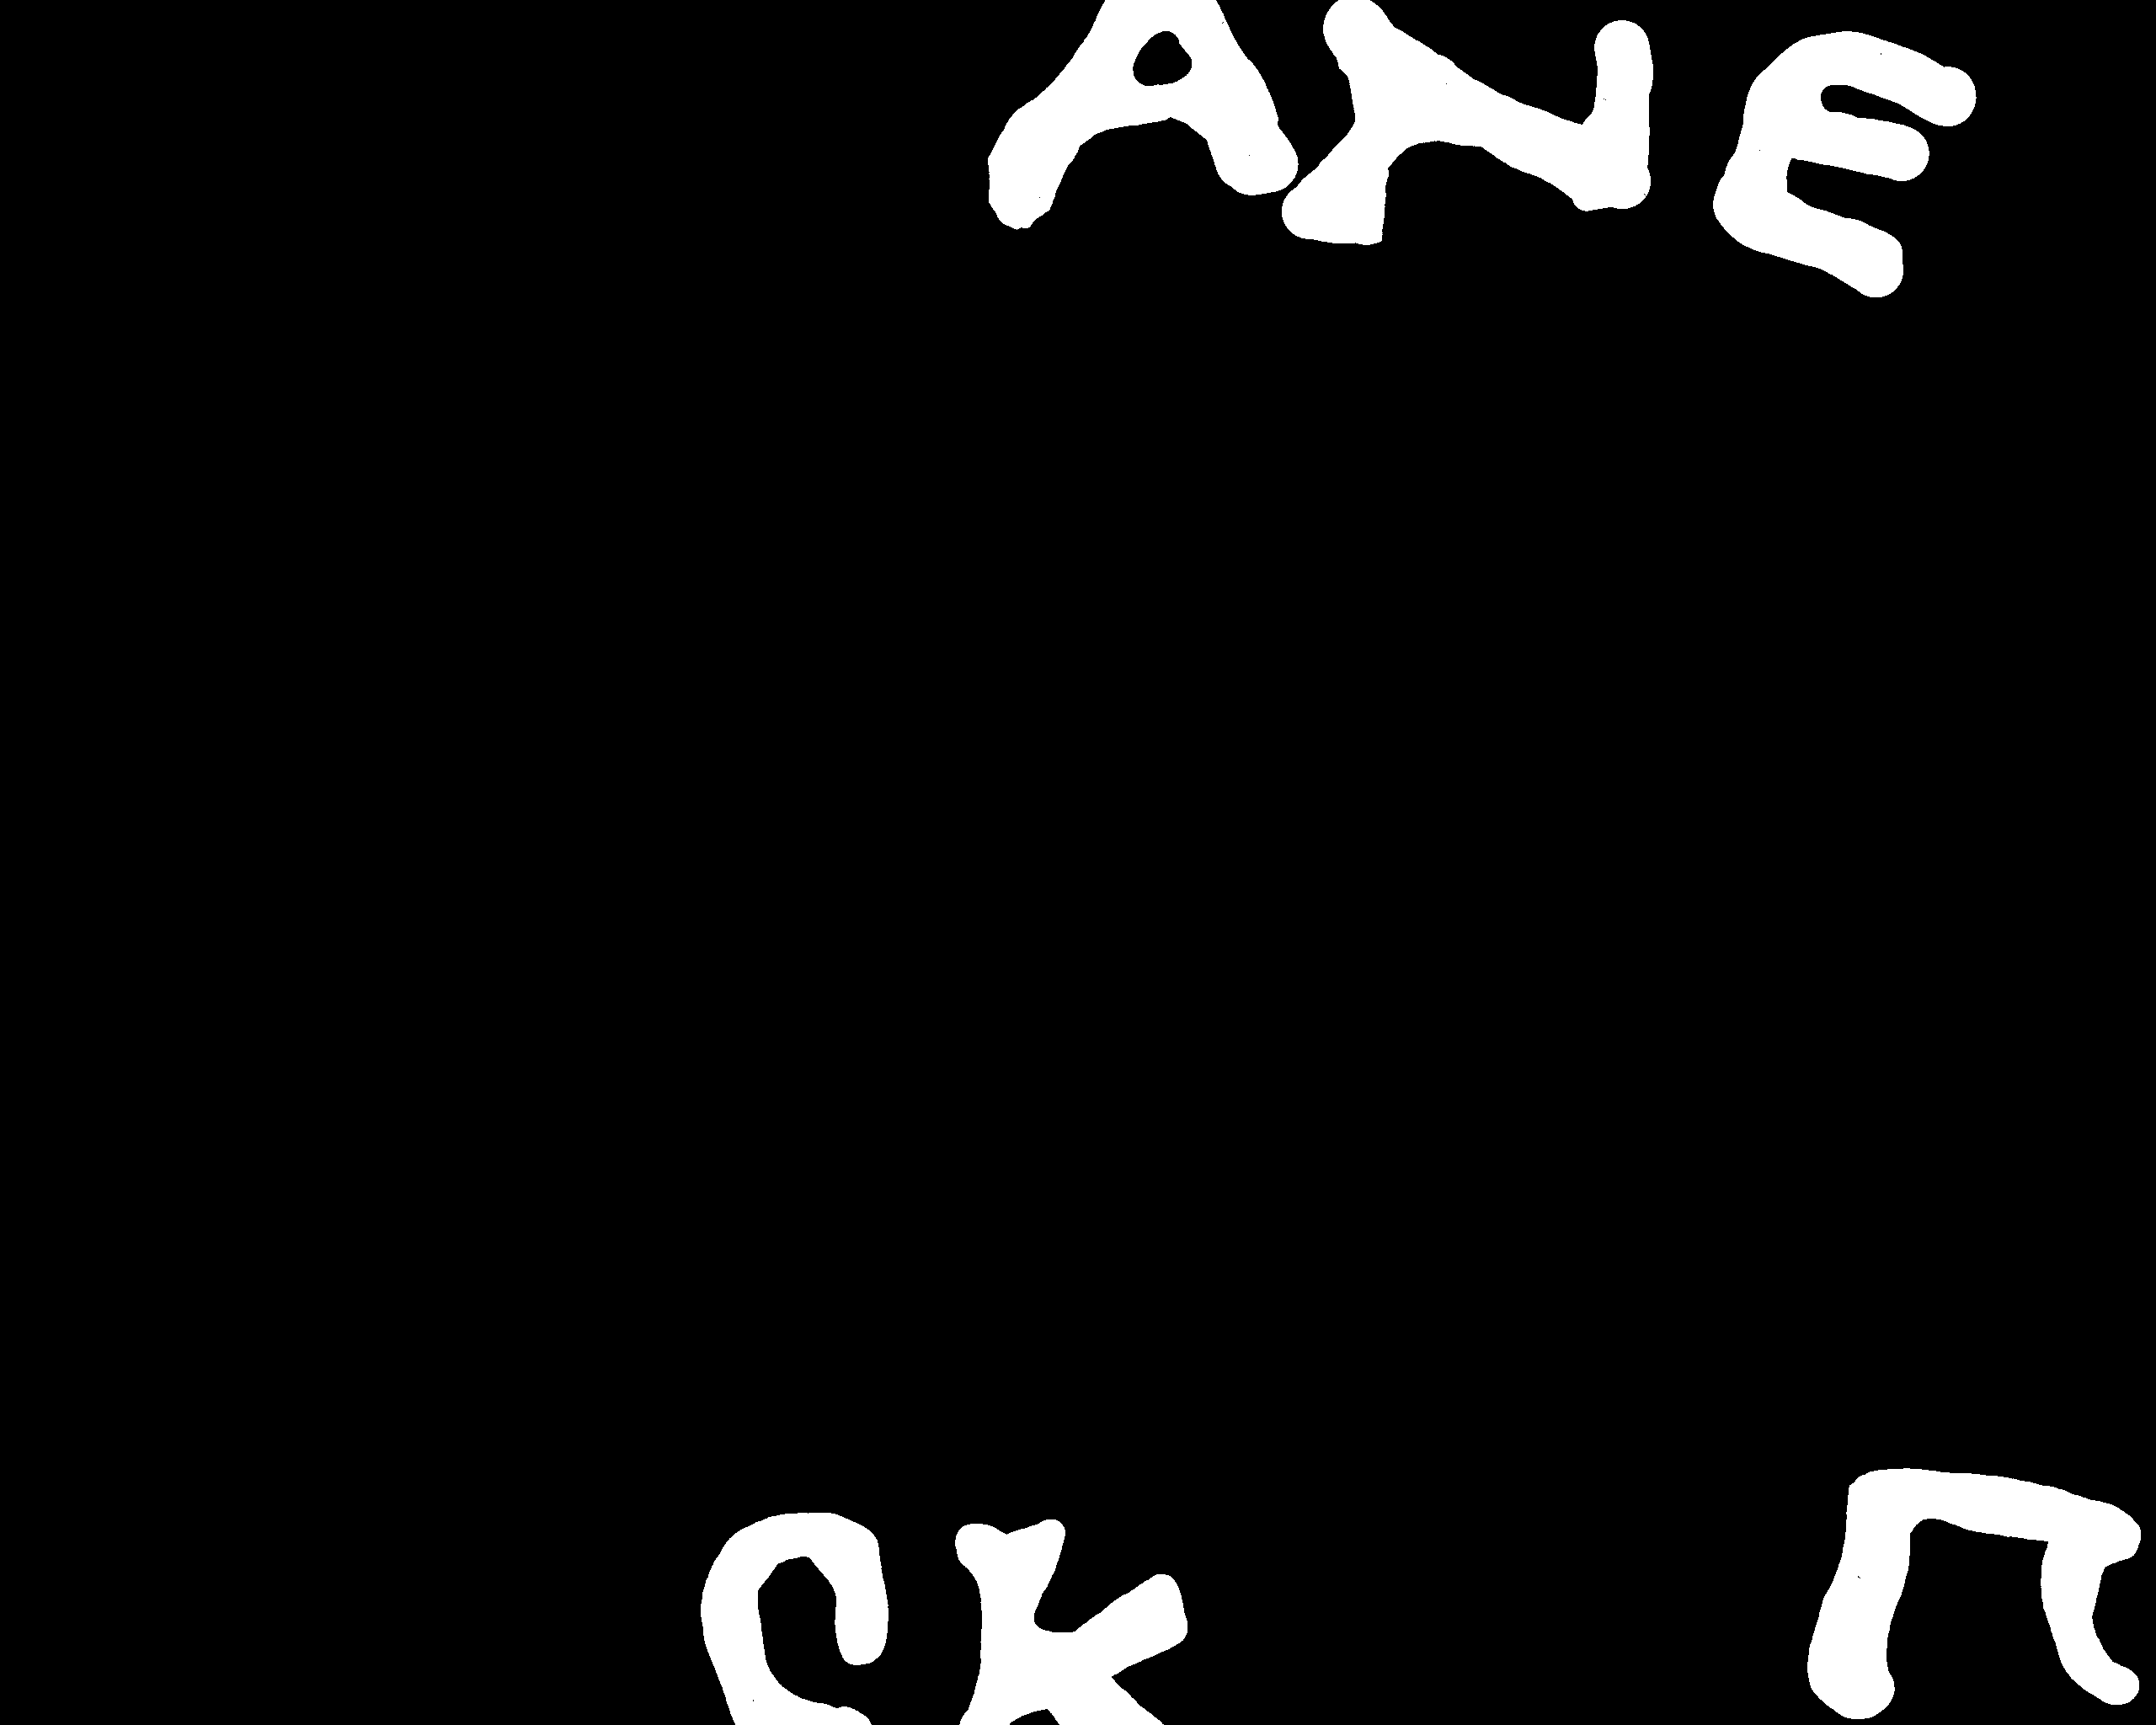
\includegraphics[width=122.48pt]{../figures/ag1/ag1_2_labels.png}}\end{minipage}}
\par\vspace{4pt}
\noindent\makebox[\columnwidth][c]{\begin{minipage}[t]{122.48pt}\centering\href{https://raw.githubusercontent.com/evilaliv3/vesuvius-challenge-pipeline/main/results/db27c806-rectina/src/figures/ag1/ag1_3_reader-v2.png}{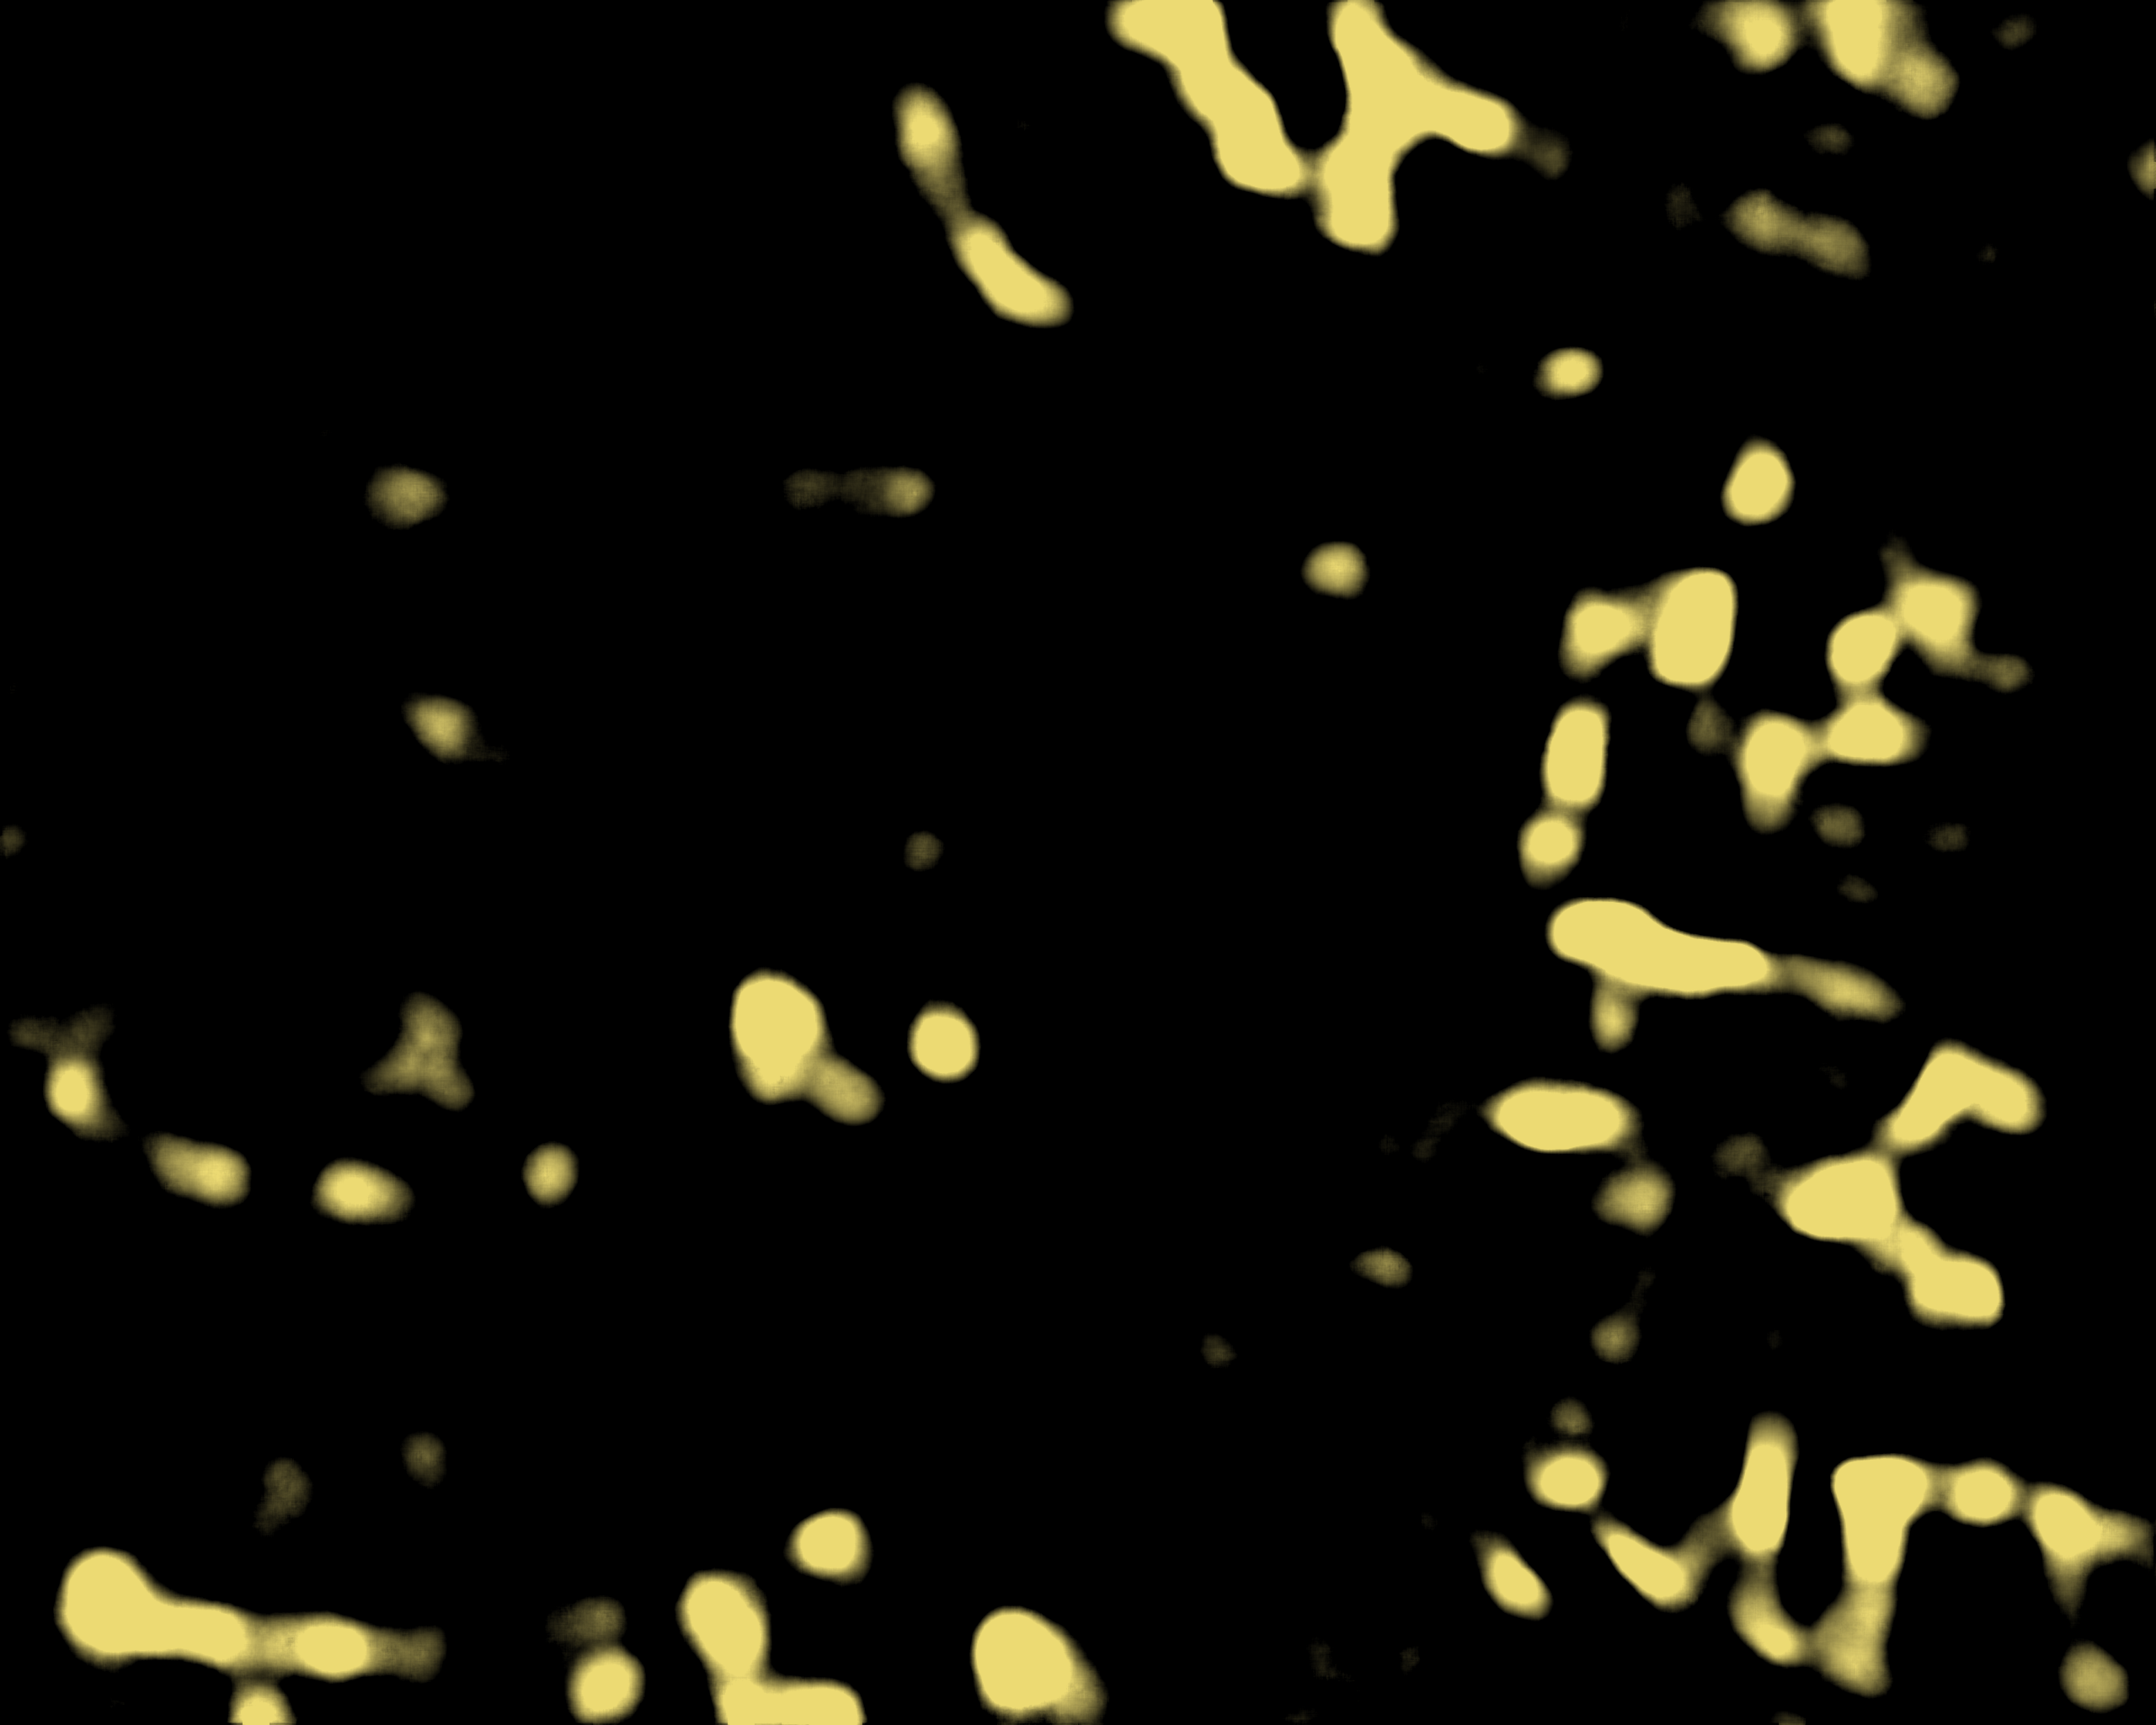
\includegraphics[width=122.48pt]{../figures/ag1/ag1_3_reader-v2.png}}\end{minipage}\hspace{2pt}\begin{minipage}[t]{122.48pt}\centering\href{https://raw.githubusercontent.com/evilaliv3/vesuvius-challenge-pipeline/main/results/db27c806-rectina/src/figures/ag1/ag1_5_rectina-m1.png}{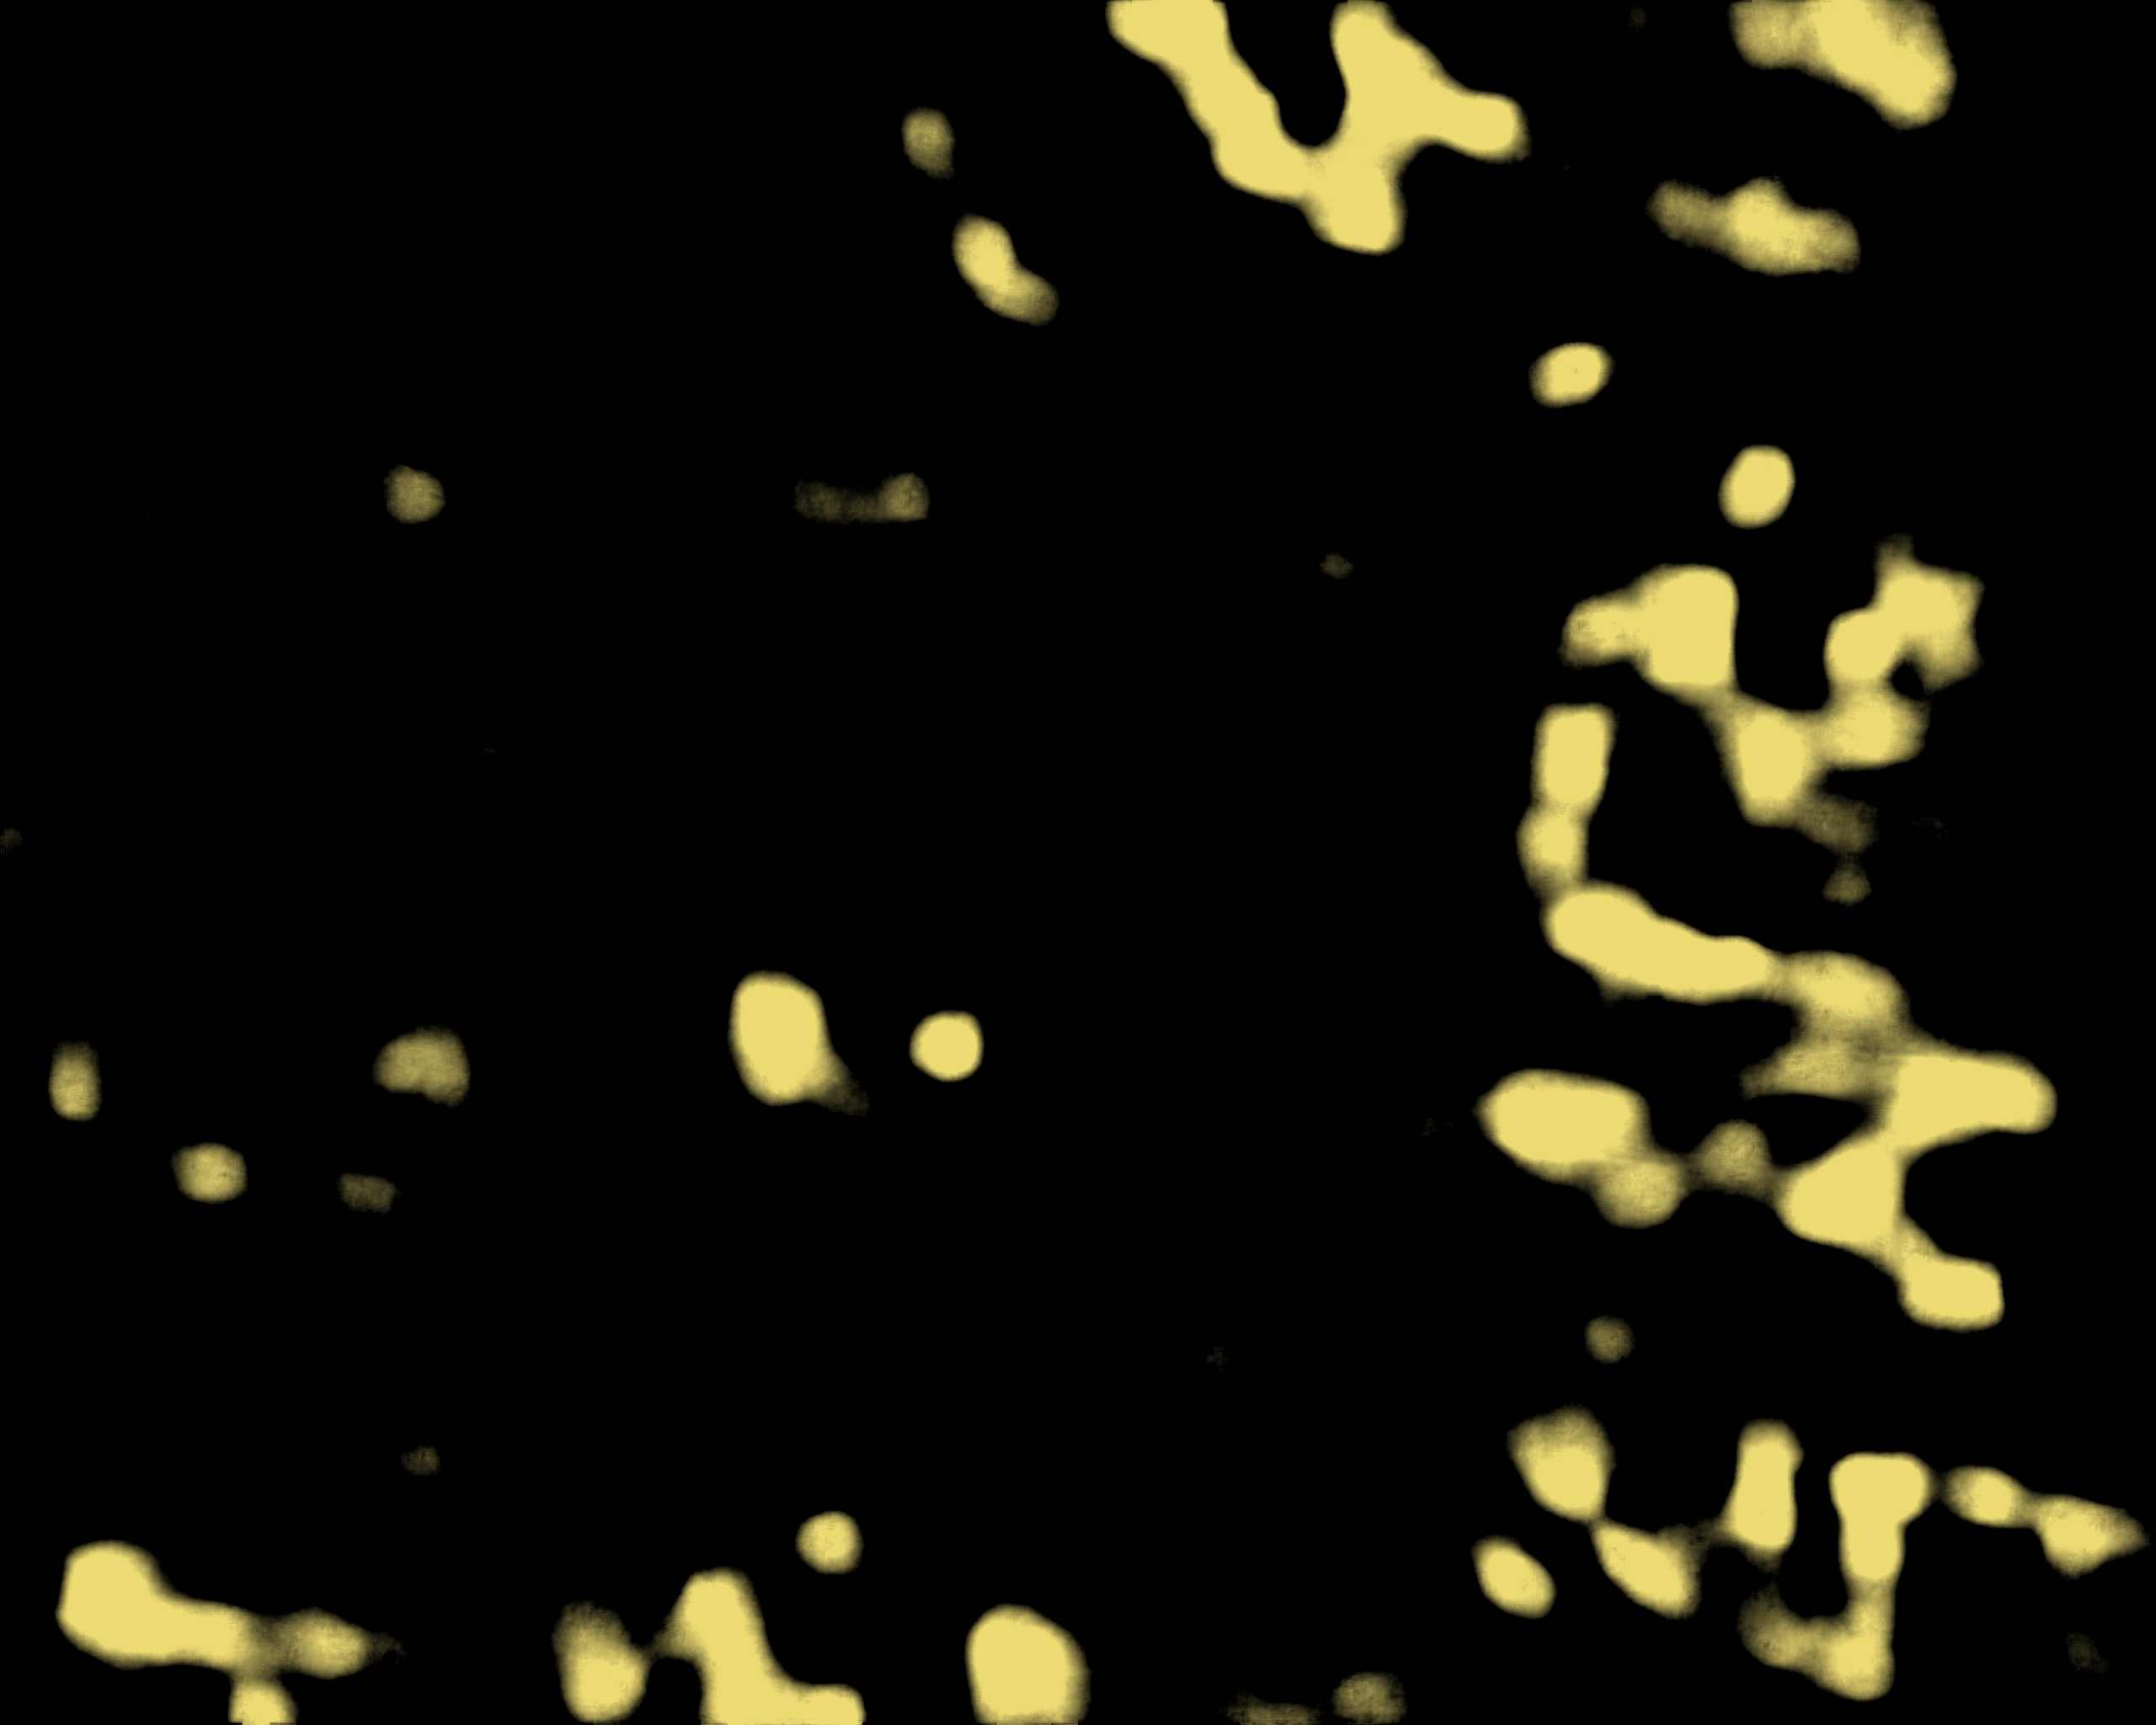
\includegraphics[width=122.48pt]{../figures/ag1/ag1_5_rectina-m1.png}}\end{minipage}}
\par\vspace{4pt}
\noindent\makebox[\columnwidth][c]{\begin{minipage}[t]{122.48pt}\centering\href{https://raw.githubusercontent.com/evilaliv3/vesuvius-challenge-pipeline/main/results/db27c806-rectina/src/figures/ag1/ag1_4_reader-v3.png}{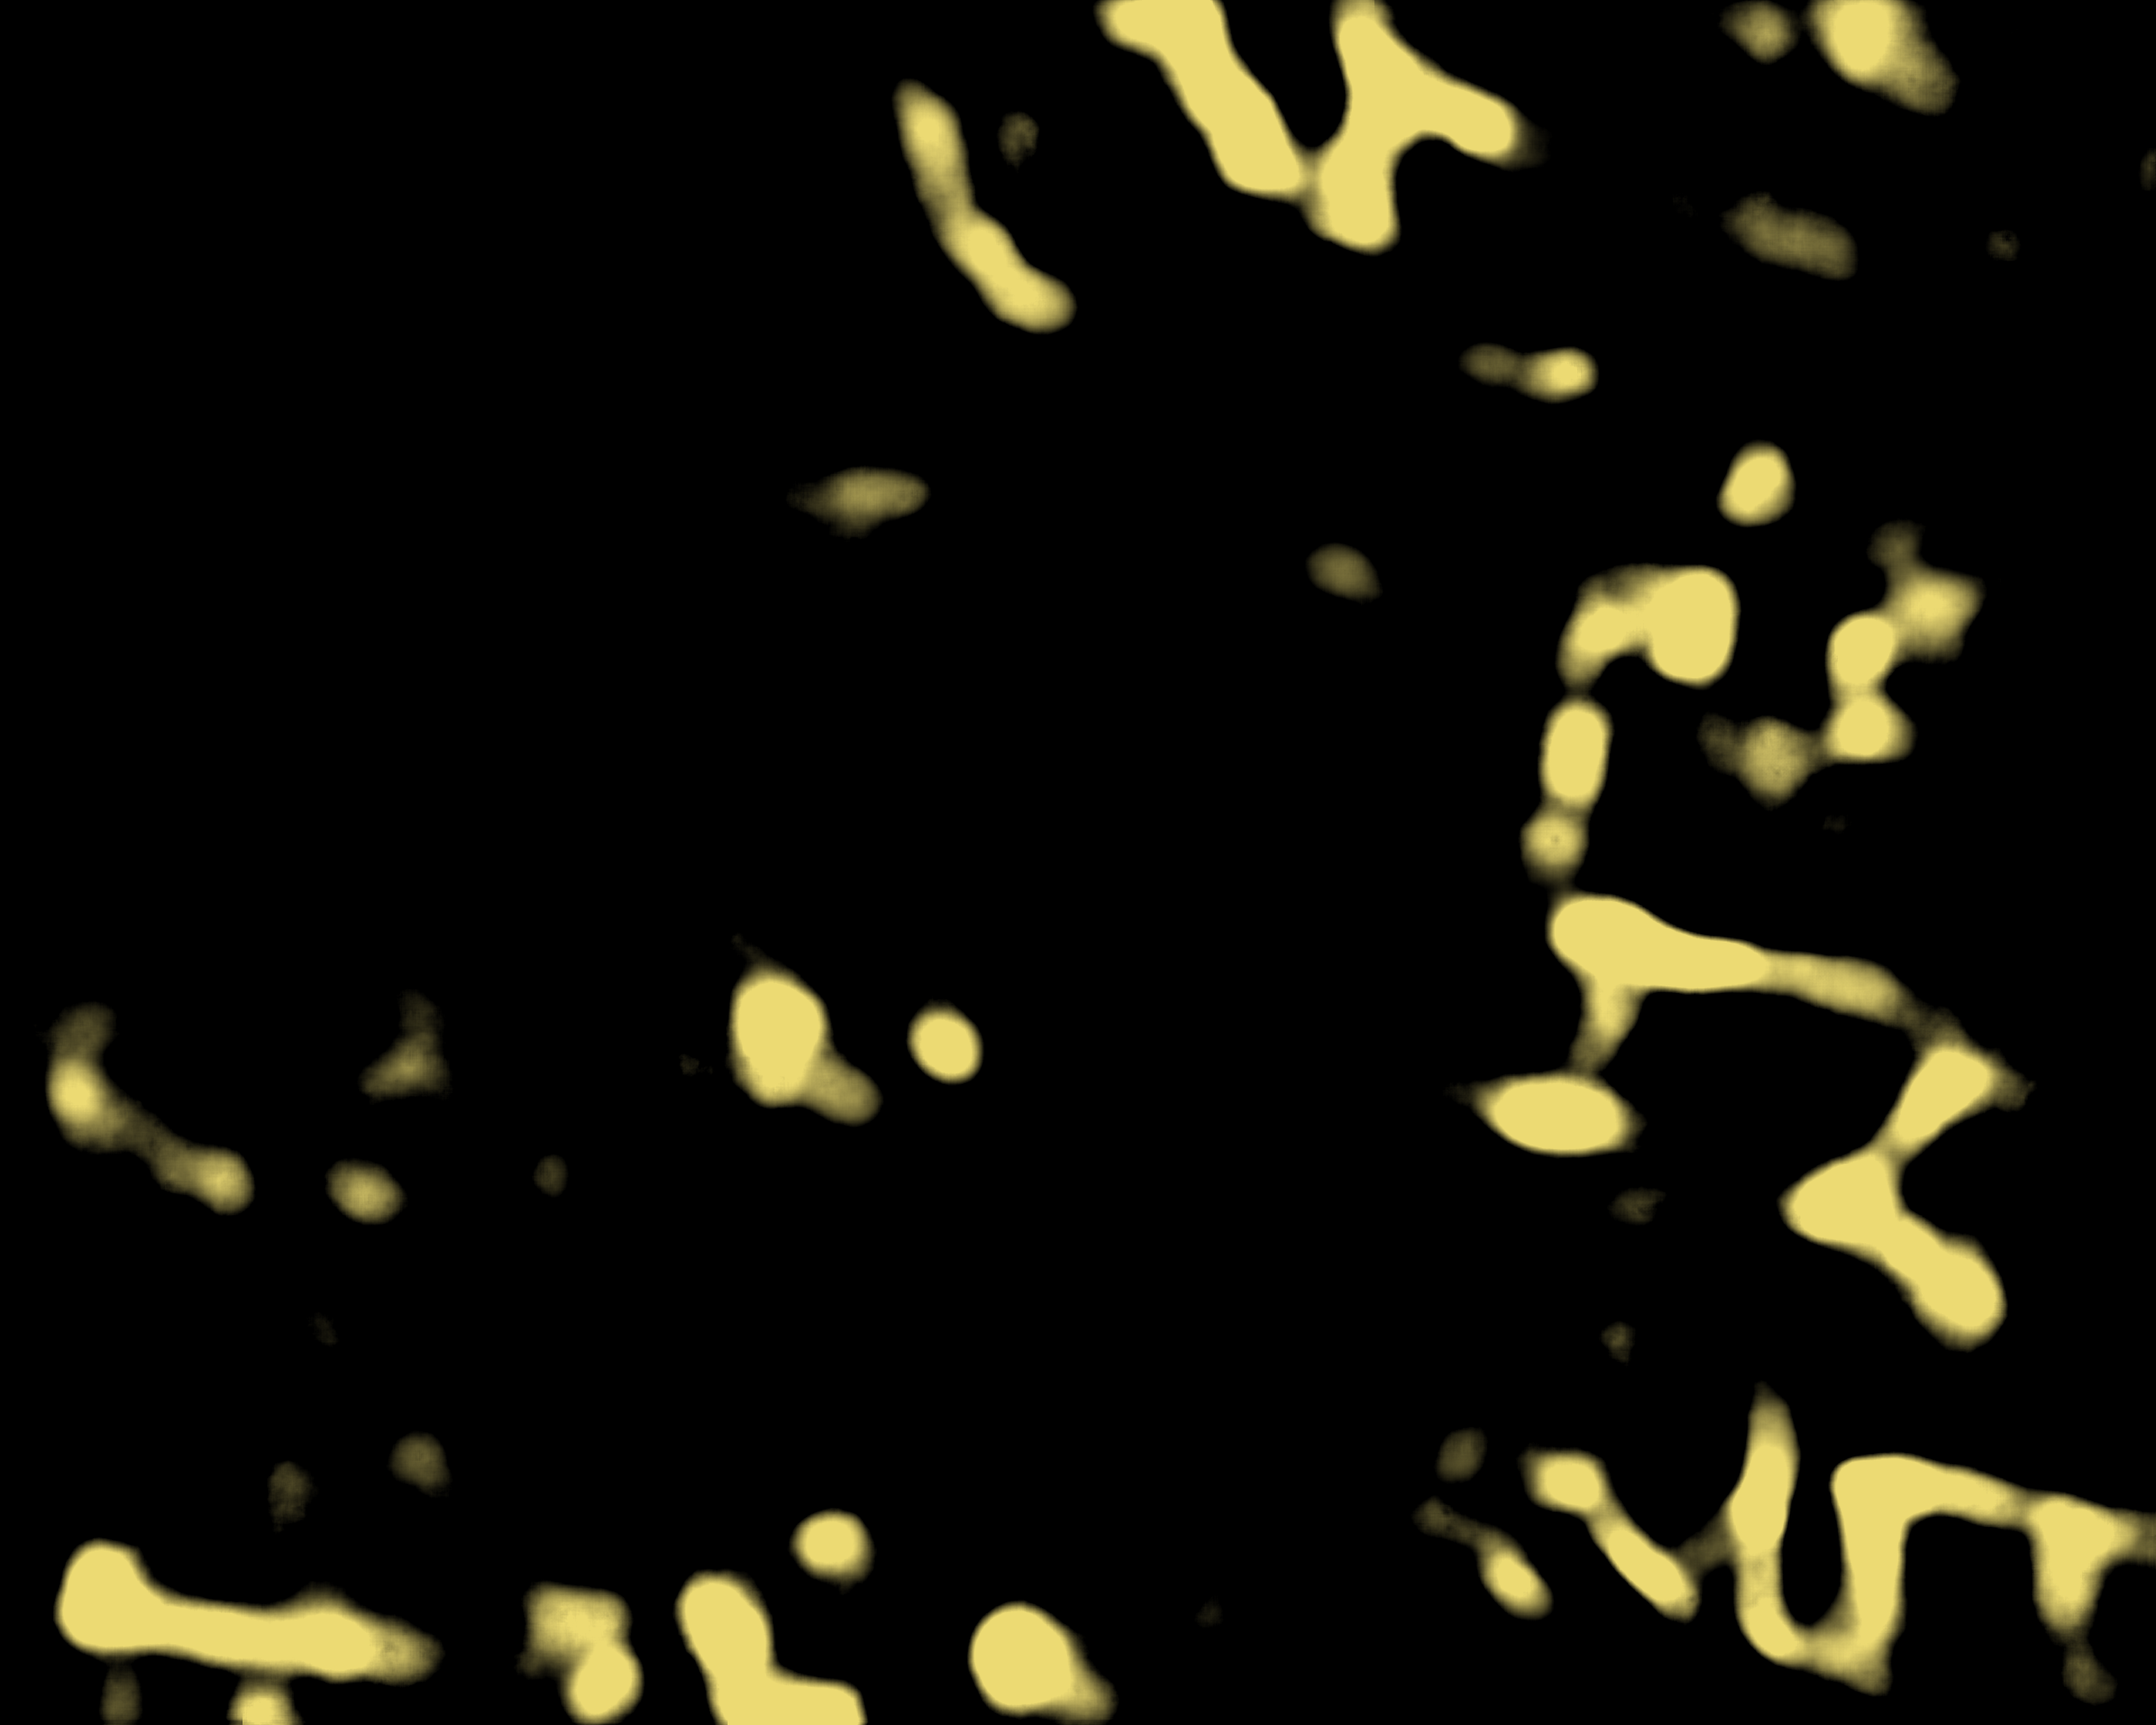
\includegraphics[width=122.48pt]{../figures/ag1/ag1_4_reader-v3.png}}\end{minipage}\hspace{2pt}\begin{minipage}[t]{122.48pt}\centering\href{https://raw.githubusercontent.com/evilaliv3/vesuvius-challenge-pipeline/main/results/db27c806-rectina/src/figures/ag1/ag1_6_rectina-m2.png}{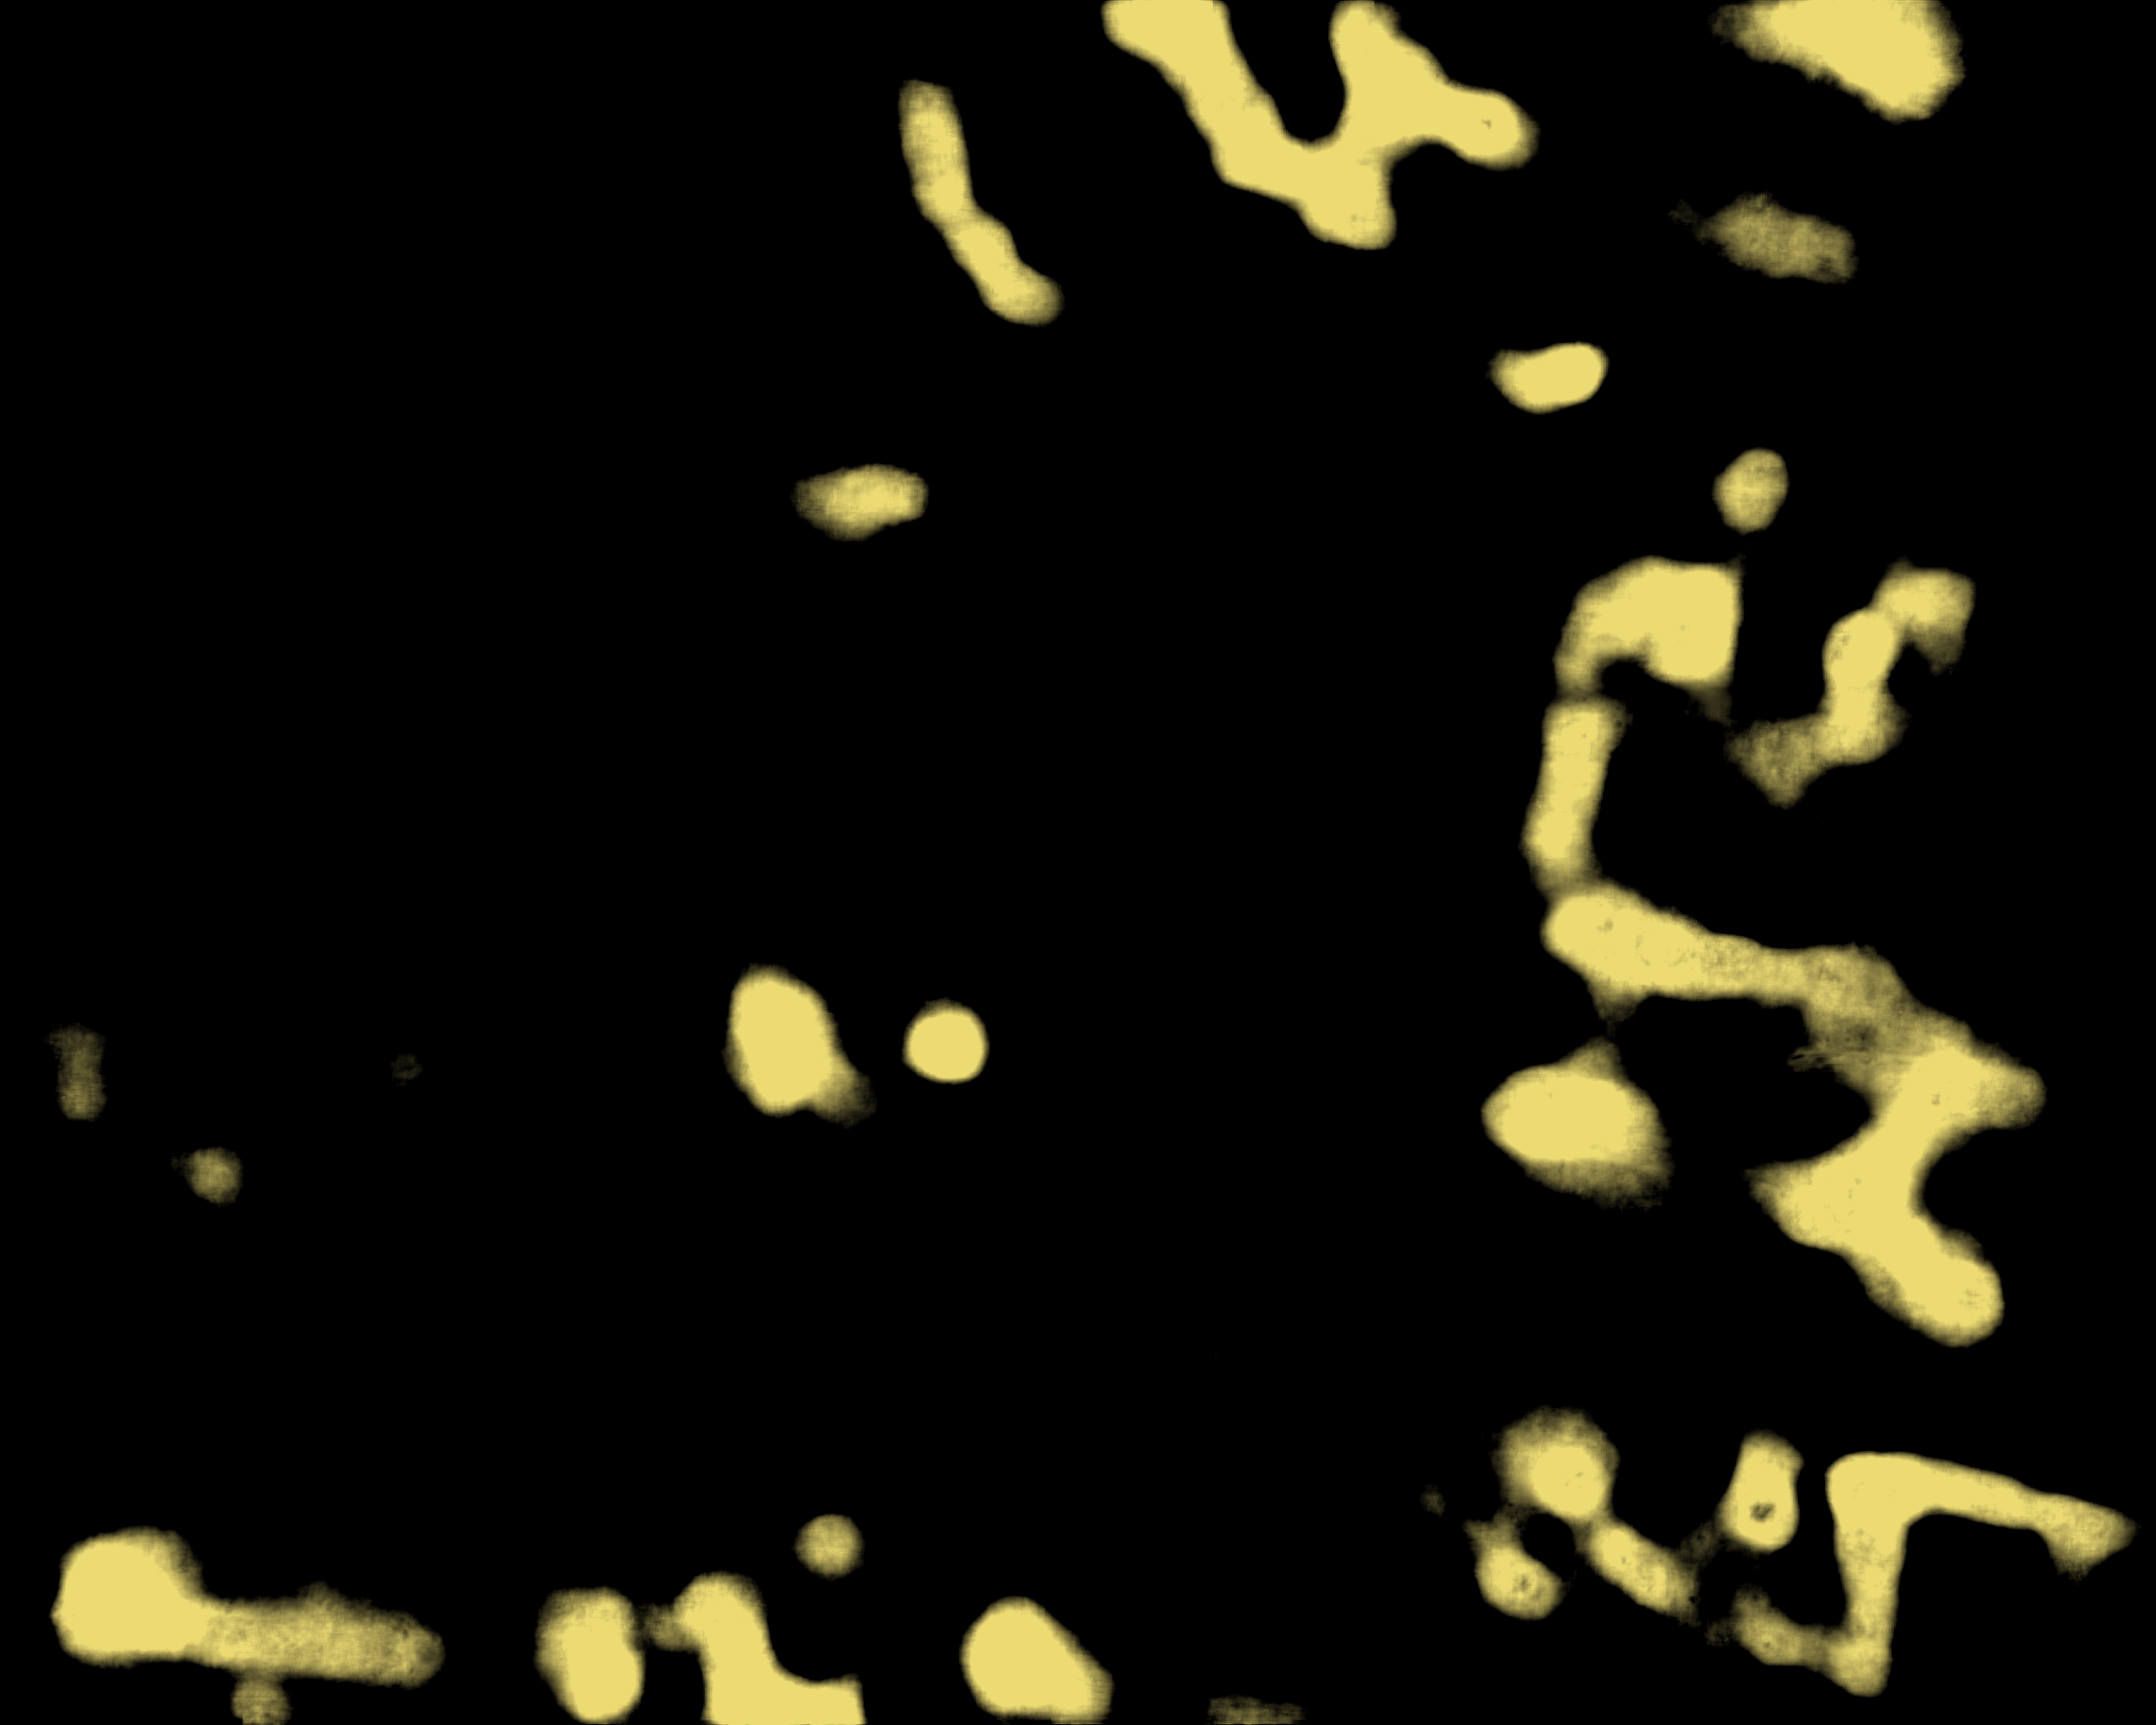
\includegraphics[width=122.48pt]{../figures/ag1/ag1_6_rectina-m2.png}}\end{minipage}}
\caption{Control unit 0841 ag1, three rows of two panels. Row 1: left, Texture; right, Labels. Row 2: left, Reader v2; right, Rectina m1 (display windows: Reader v2 0.447222 to 0.621051 (ramp); Rectina m1 0.623262 to 0.741702 (ramp)). Row 3: left, Reader v3; right, Rectina m2 (display windows: Reader v3 0.470294 to 0.693186 (ramp); Rectina m2 0.671638 to 0.774498 (ramp)). Each map is stretched between its own percentiles. Reader and model stand side by side in the rows 2 and 3.}
\end{figure}

\begin{figure}[!tbp]
\centering
\noindent\makebox[\columnwidth][c]{\begin{minipage}[t]{122.48pt}\centering\href{https://raw.githubusercontent.com/evilaliv3/vesuvius-challenge-pipeline/main/results/db27c806-rectina/src/figures/ag2/ag2_1_texture.png}{
\includegraphics[width=122.48pt]{../figures/ag2/ag2_1_texture.png}}\end{minipage}\hspace{2pt}\begin{minipage}[t]{122.48pt}\centering\href{https://raw.githubusercontent.com/evilaliv3/vesuvius-challenge-pipeline/main/results/db27c806-rectina/src/figures/ag2/ag2_2_labels.png}{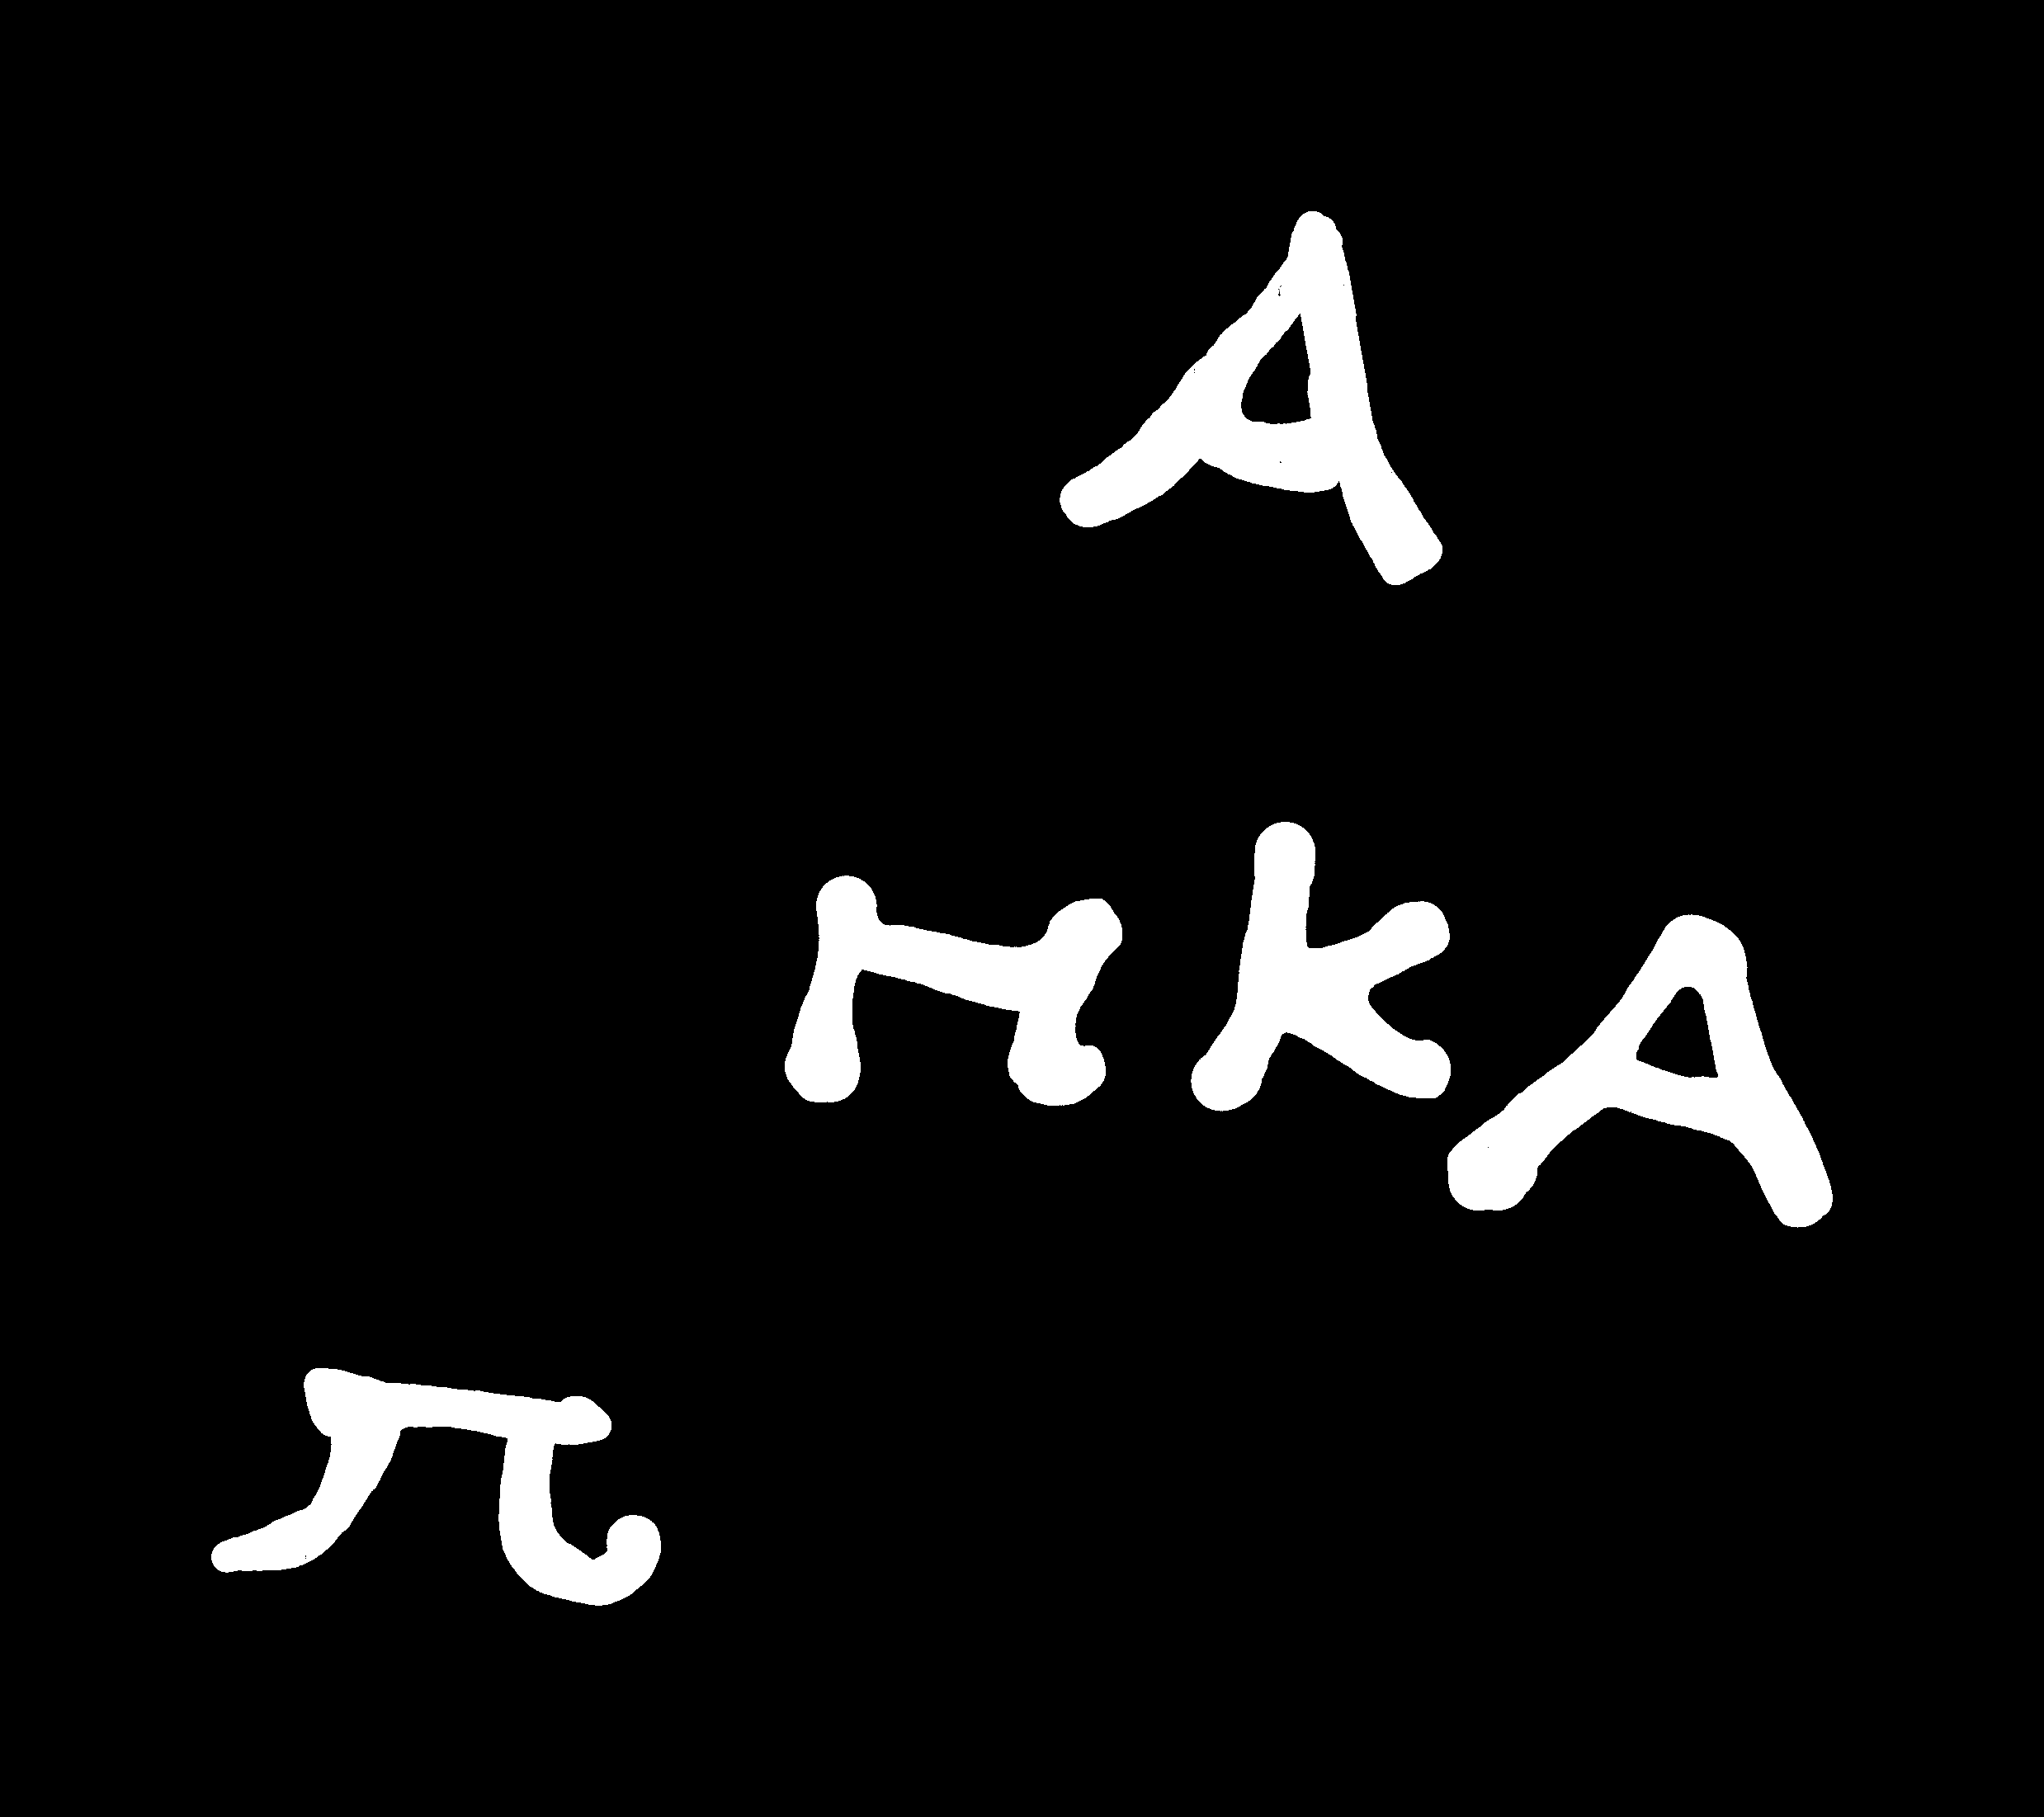
\includegraphics[width=122.48pt]{../figures/ag2/ag2_2_labels.png}}\end{minipage}}
\par\vspace{4pt}
\noindent\makebox[\columnwidth][c]{\begin{minipage}[t]{122.48pt}\centering\href{https://raw.githubusercontent.com/evilaliv3/vesuvius-challenge-pipeline/main/results/db27c806-rectina/src/figures/ag2/ag2_3_reader-v2.png}{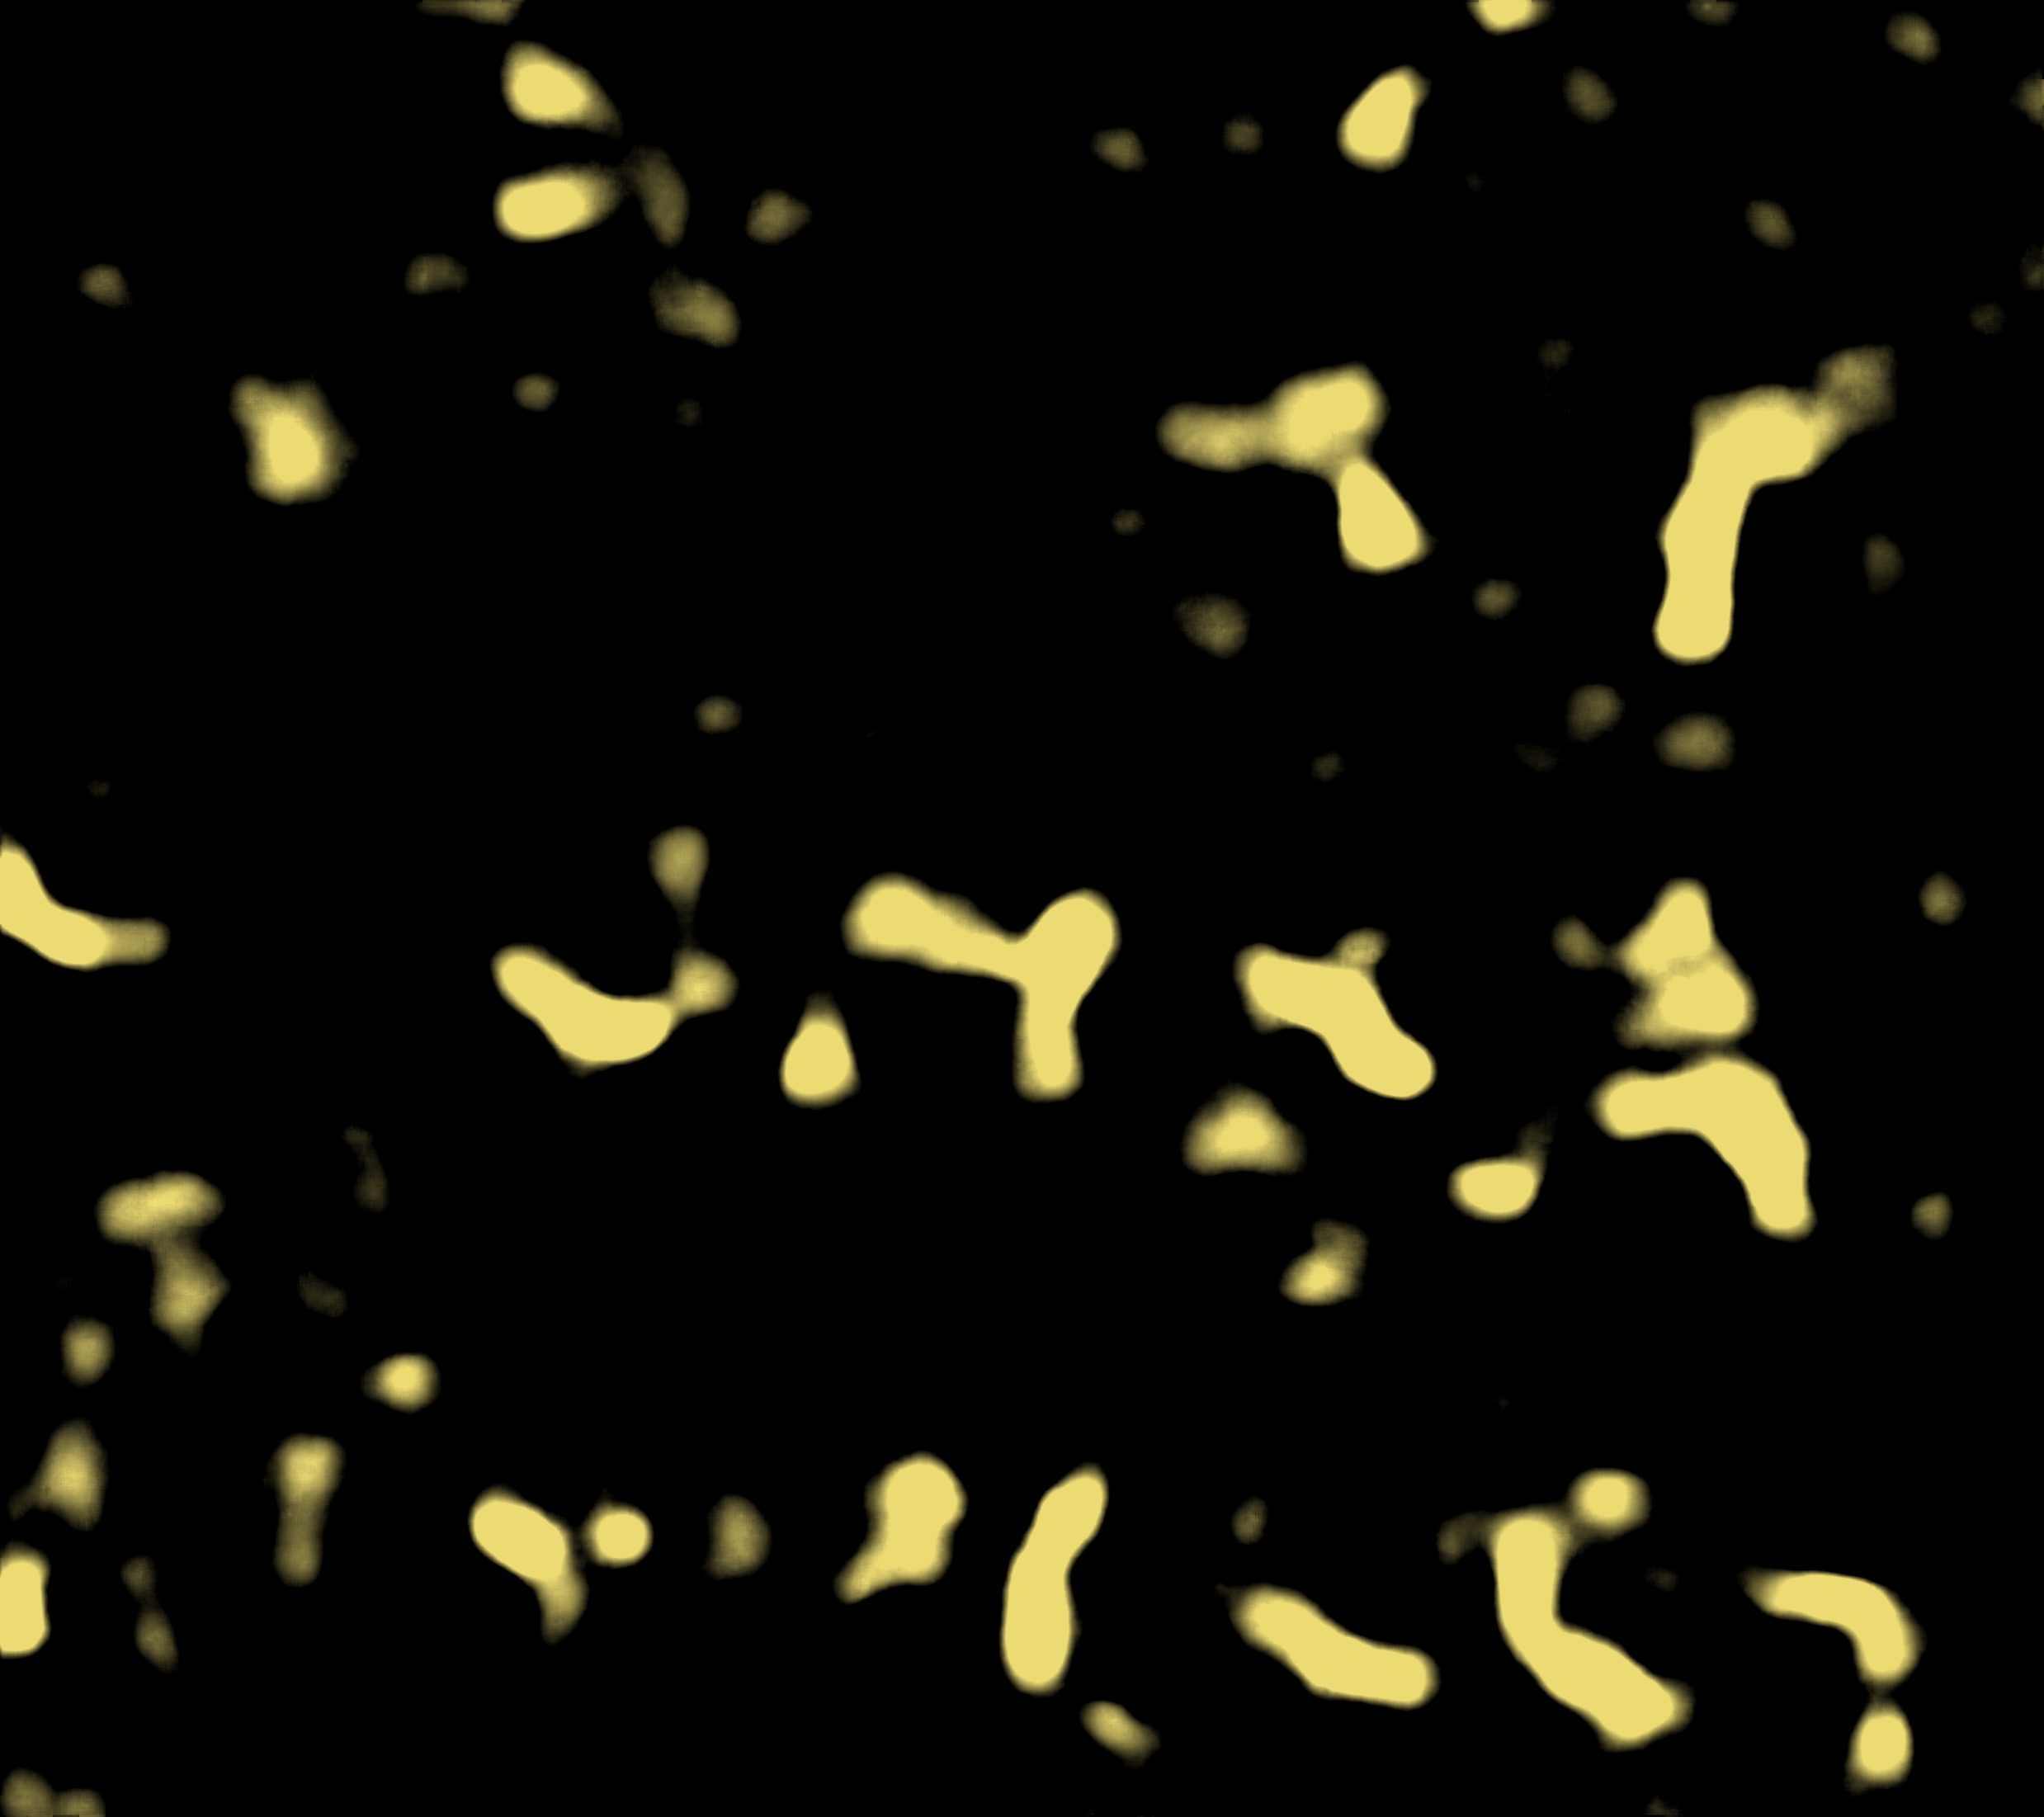
\includegraphics[width=122.48pt]{../figures/ag2/ag2_3_reader-v2.png}}\end{minipage}\hspace{2pt}\begin{minipage}[t]{122.48pt}\centering\href{https://raw.githubusercontent.com/evilaliv3/vesuvius-challenge-pipeline/main/results/db27c806-rectina/src/figures/ag2/ag2_5_rectina-m1.png}{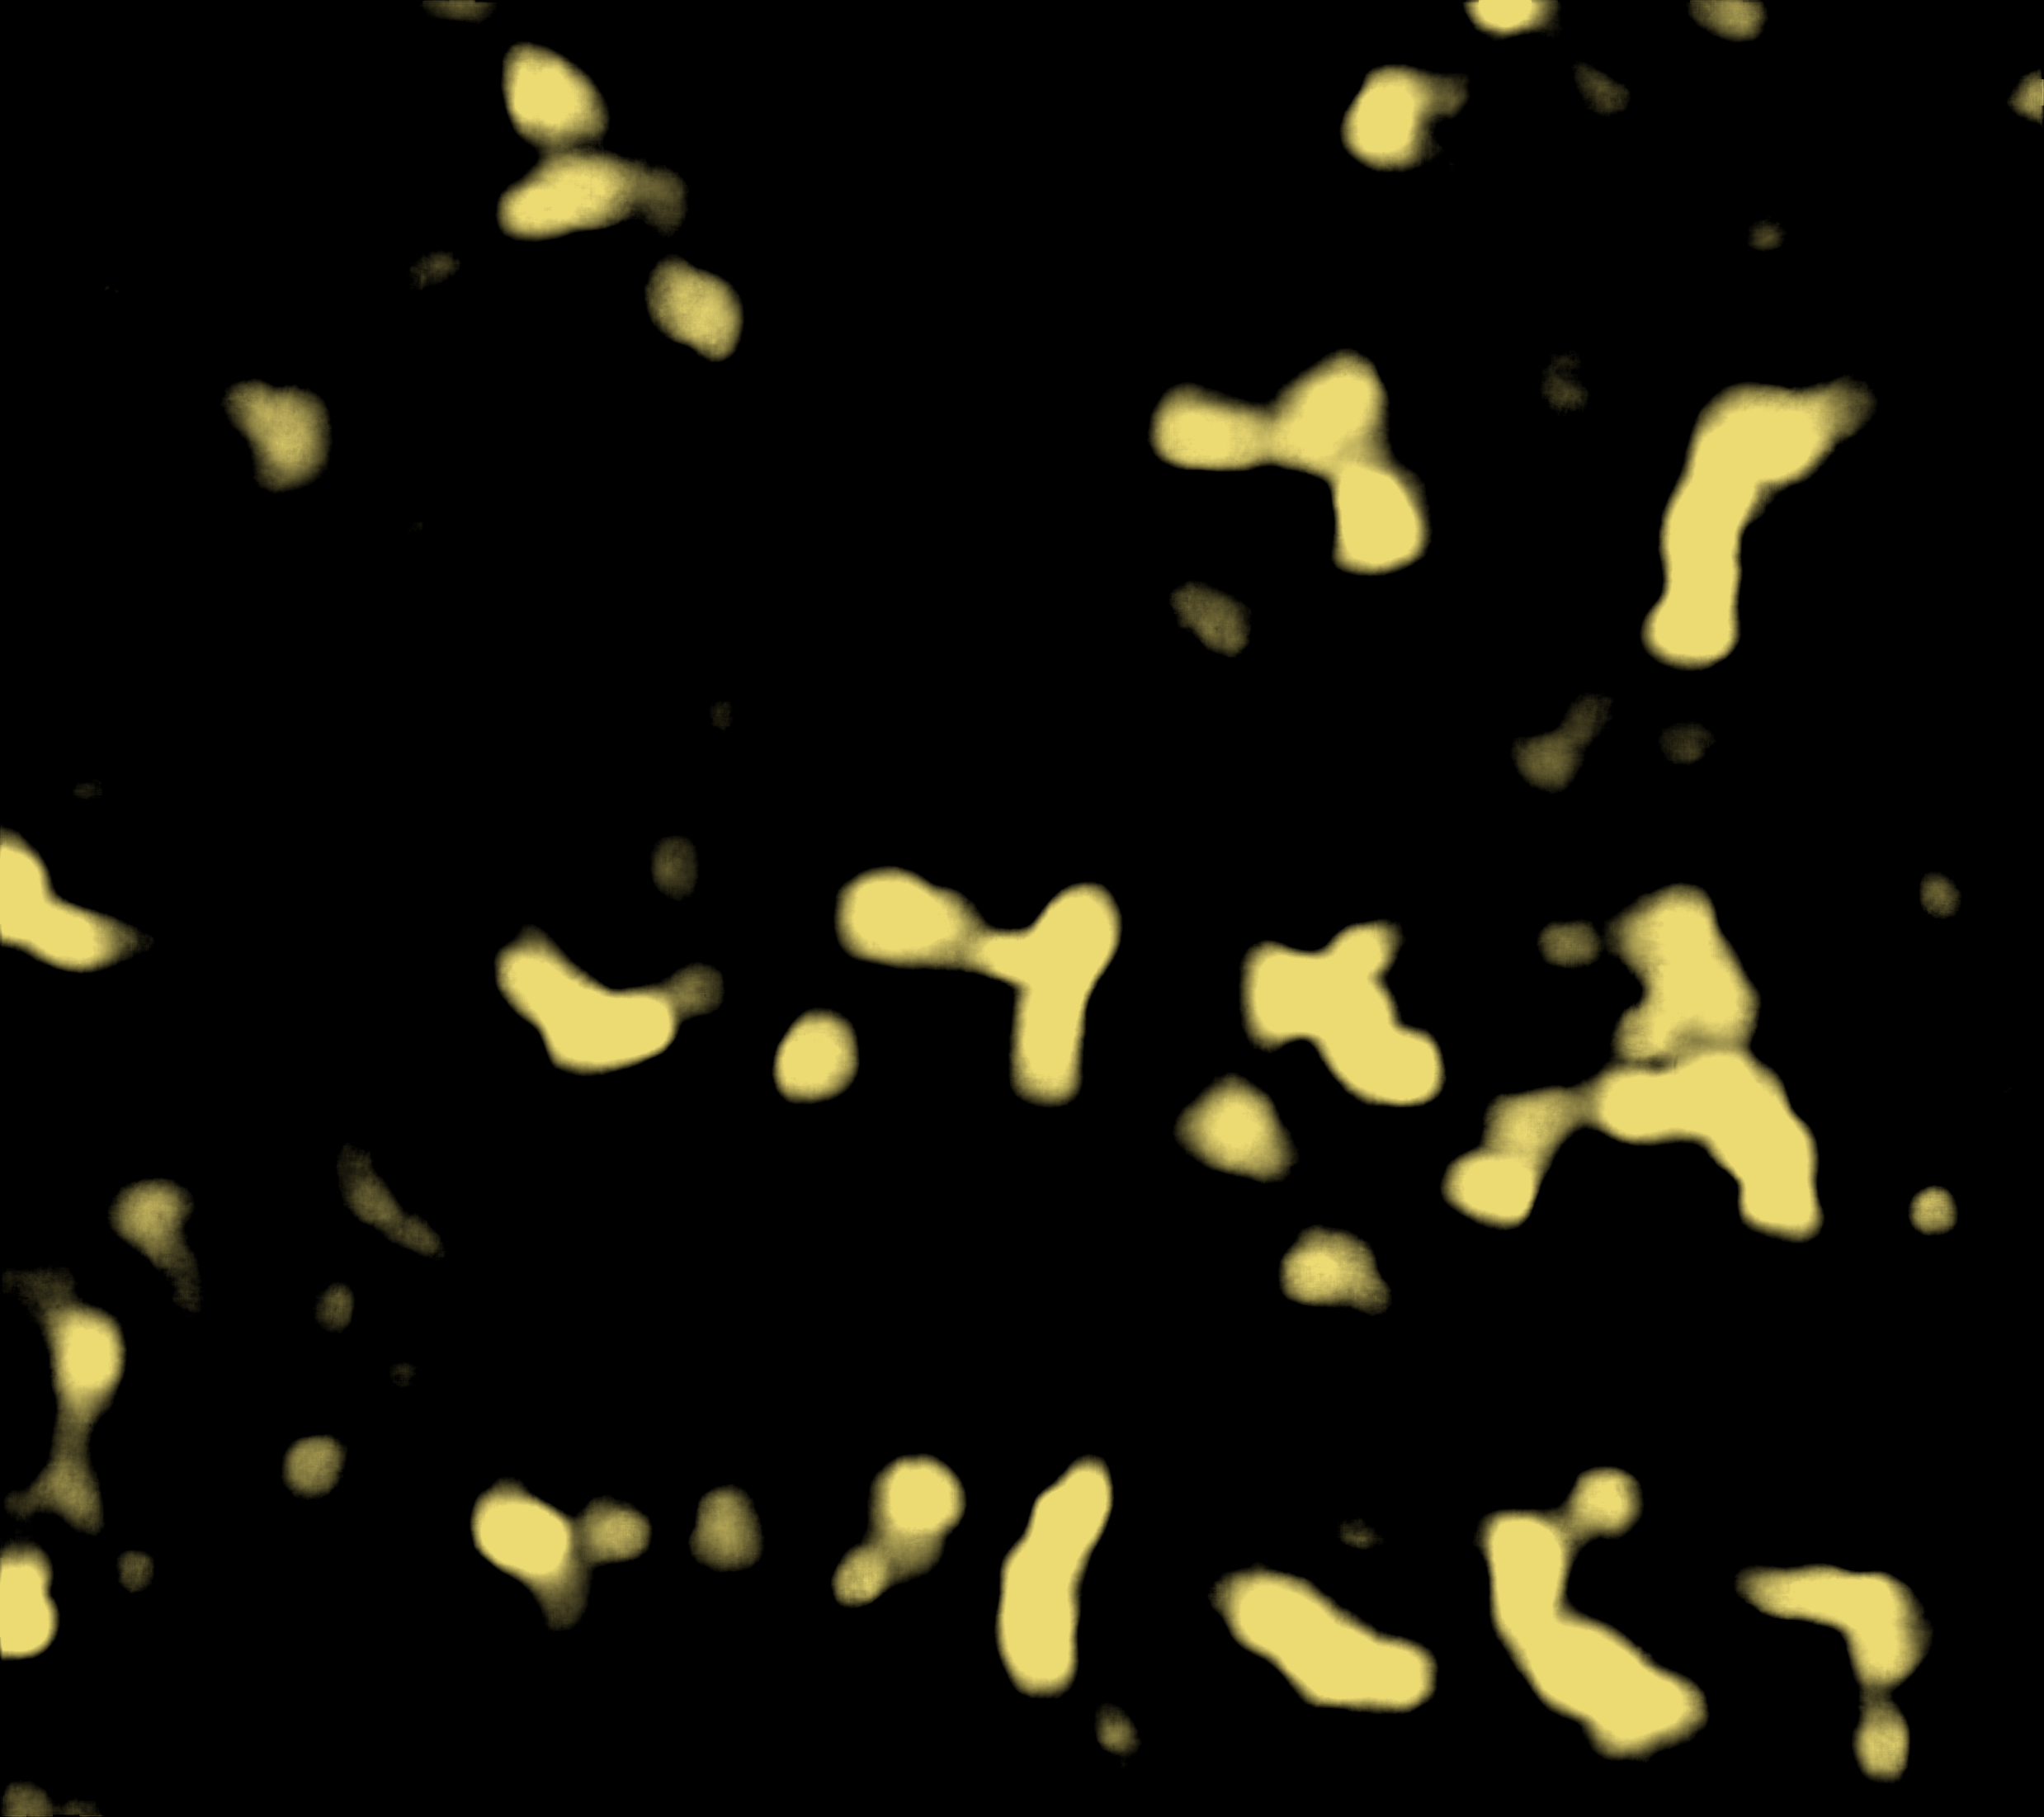
\includegraphics[width=122.48pt]{../figures/ag2/ag2_5_rectina-m1.png}}\end{minipage}}
\par\vspace{4pt}
\noindent\makebox[\columnwidth][c]{\begin{minipage}[t]{122.48pt}\centering\href{https://raw.githubusercontent.com/evilaliv3/vesuvius-challenge-pipeline/main/results/db27c806-rectina/src/figures/ag2/ag2_4_reader-v3.png}{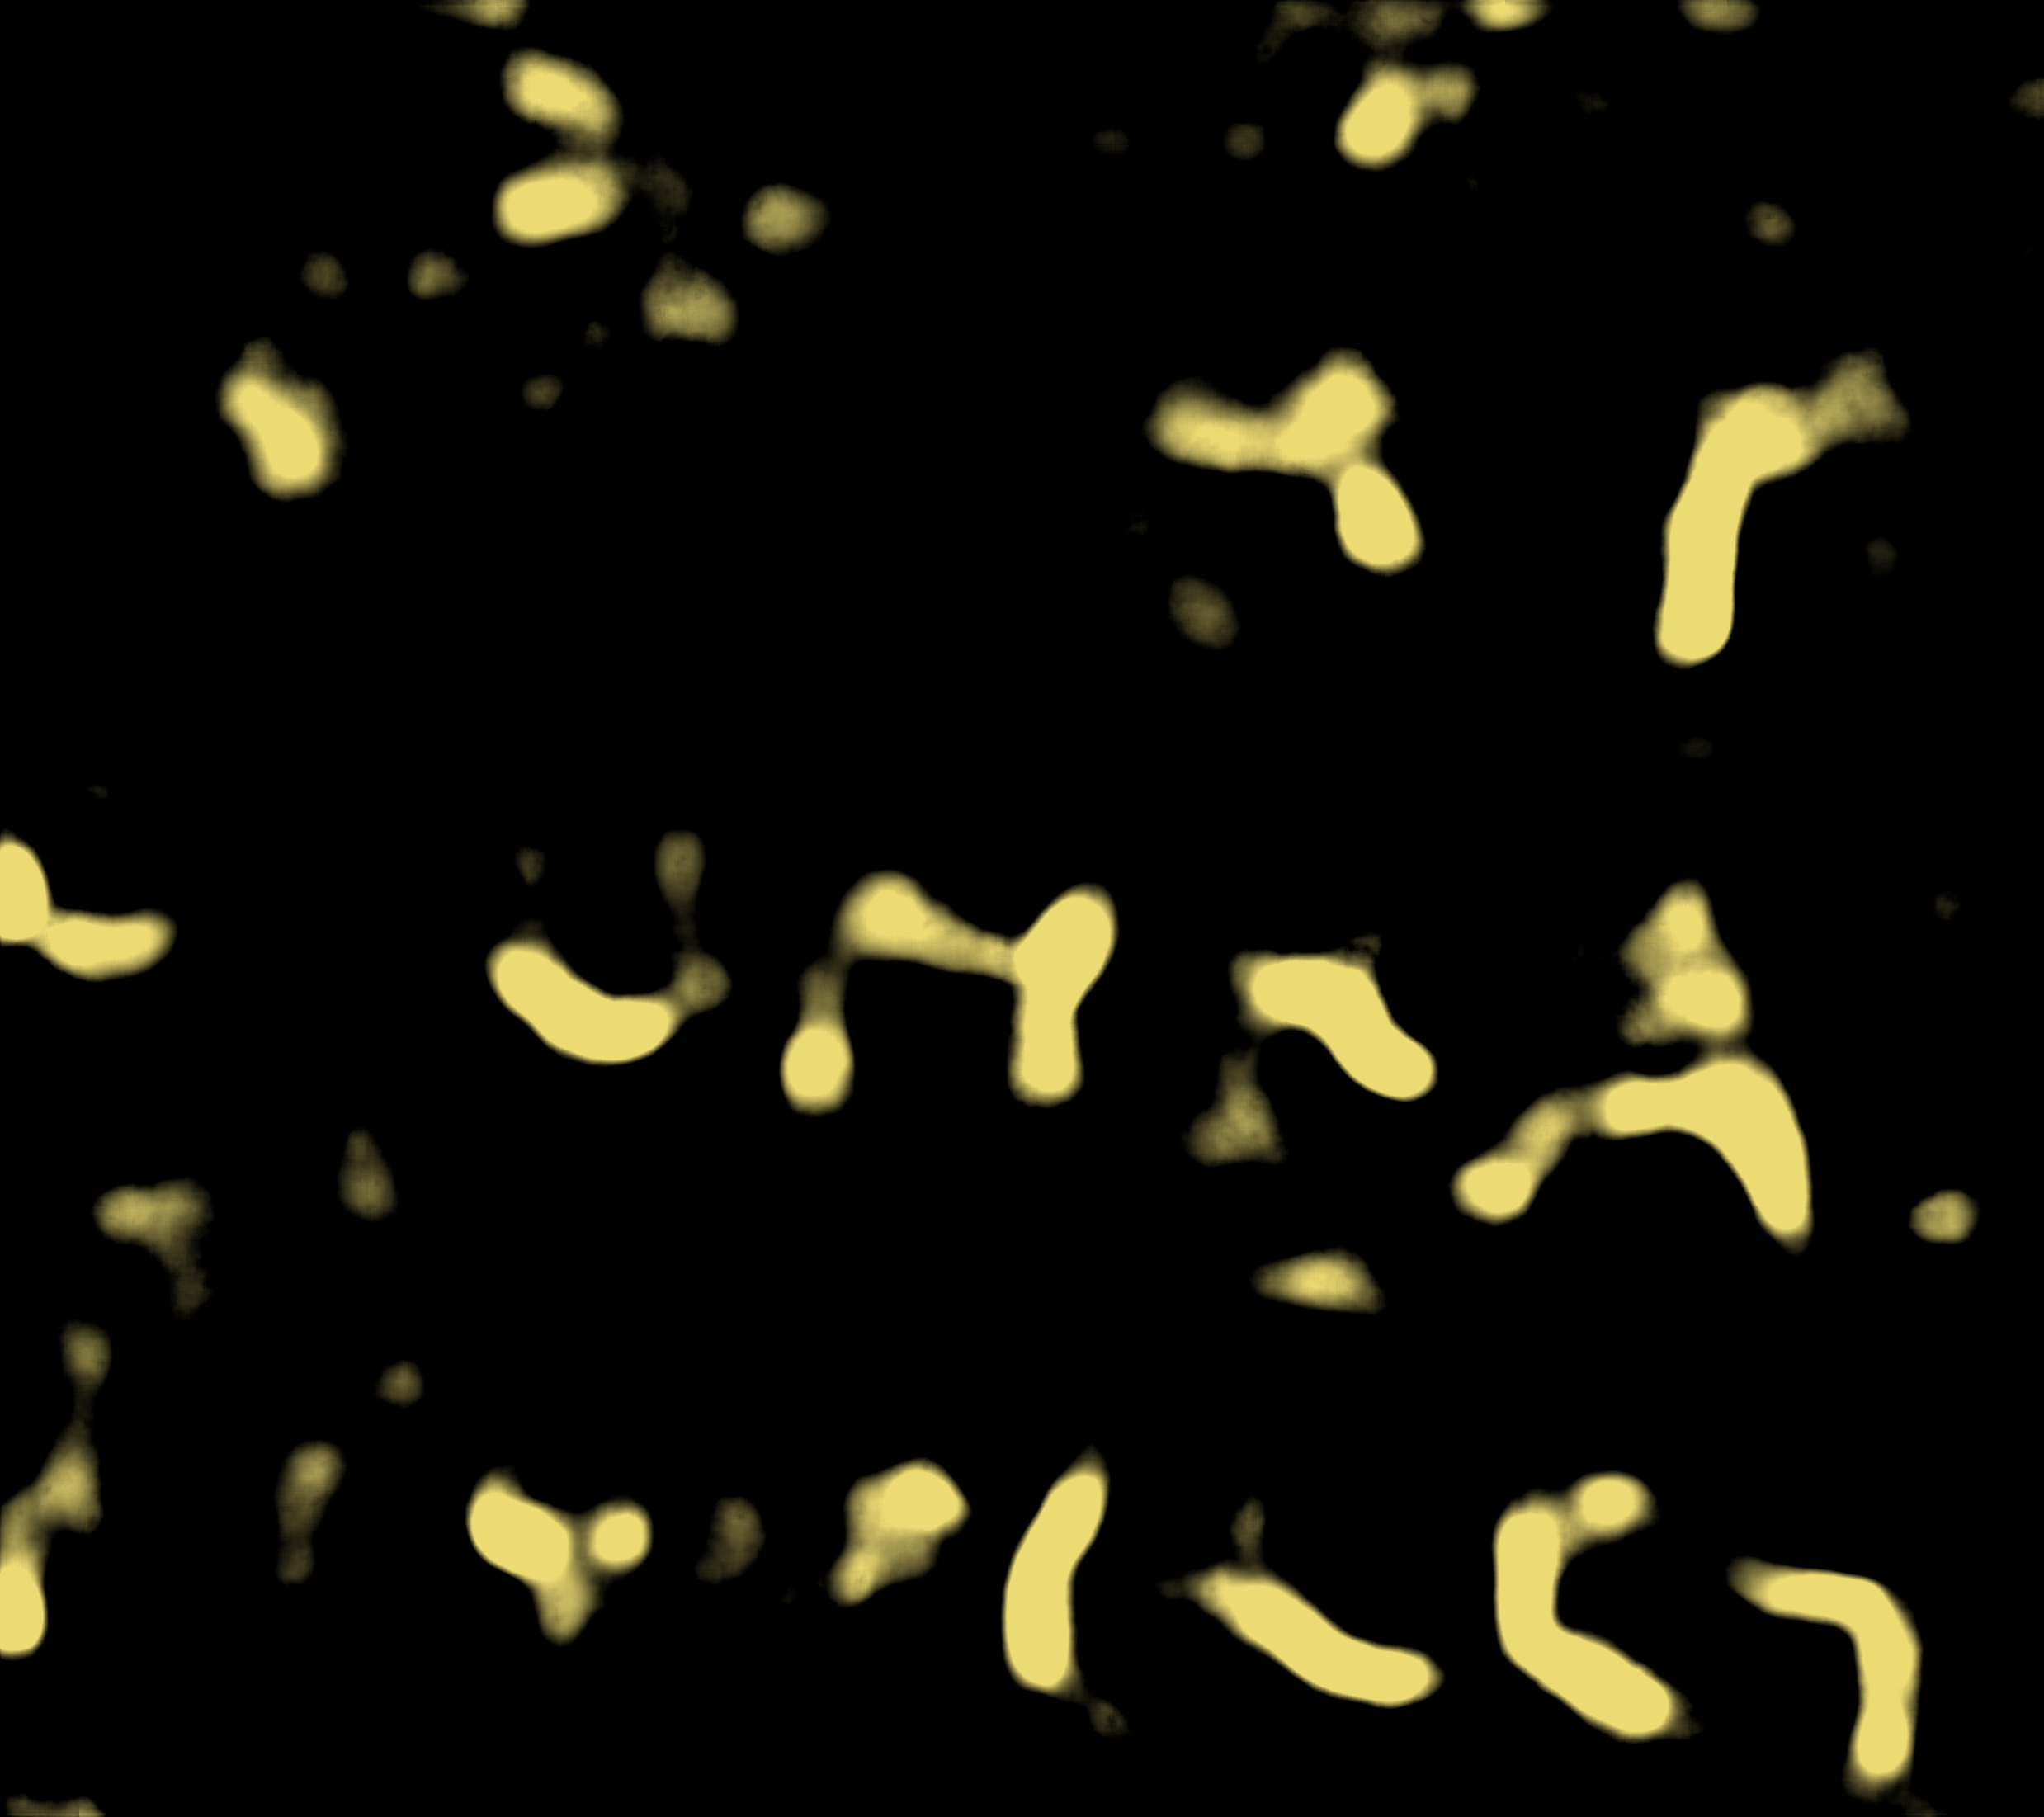
\includegraphics[width=122.48pt]{../figures/ag2/ag2_4_reader-v3.png}}\end{minipage}\hspace{2pt}\begin{minipage}[t]{122.48pt}\centering\href{https://raw.githubusercontent.com/evilaliv3/vesuvius-challenge-pipeline/main/results/db27c806-rectina/src/figures/ag2/ag2_6_rectina-m2.png}{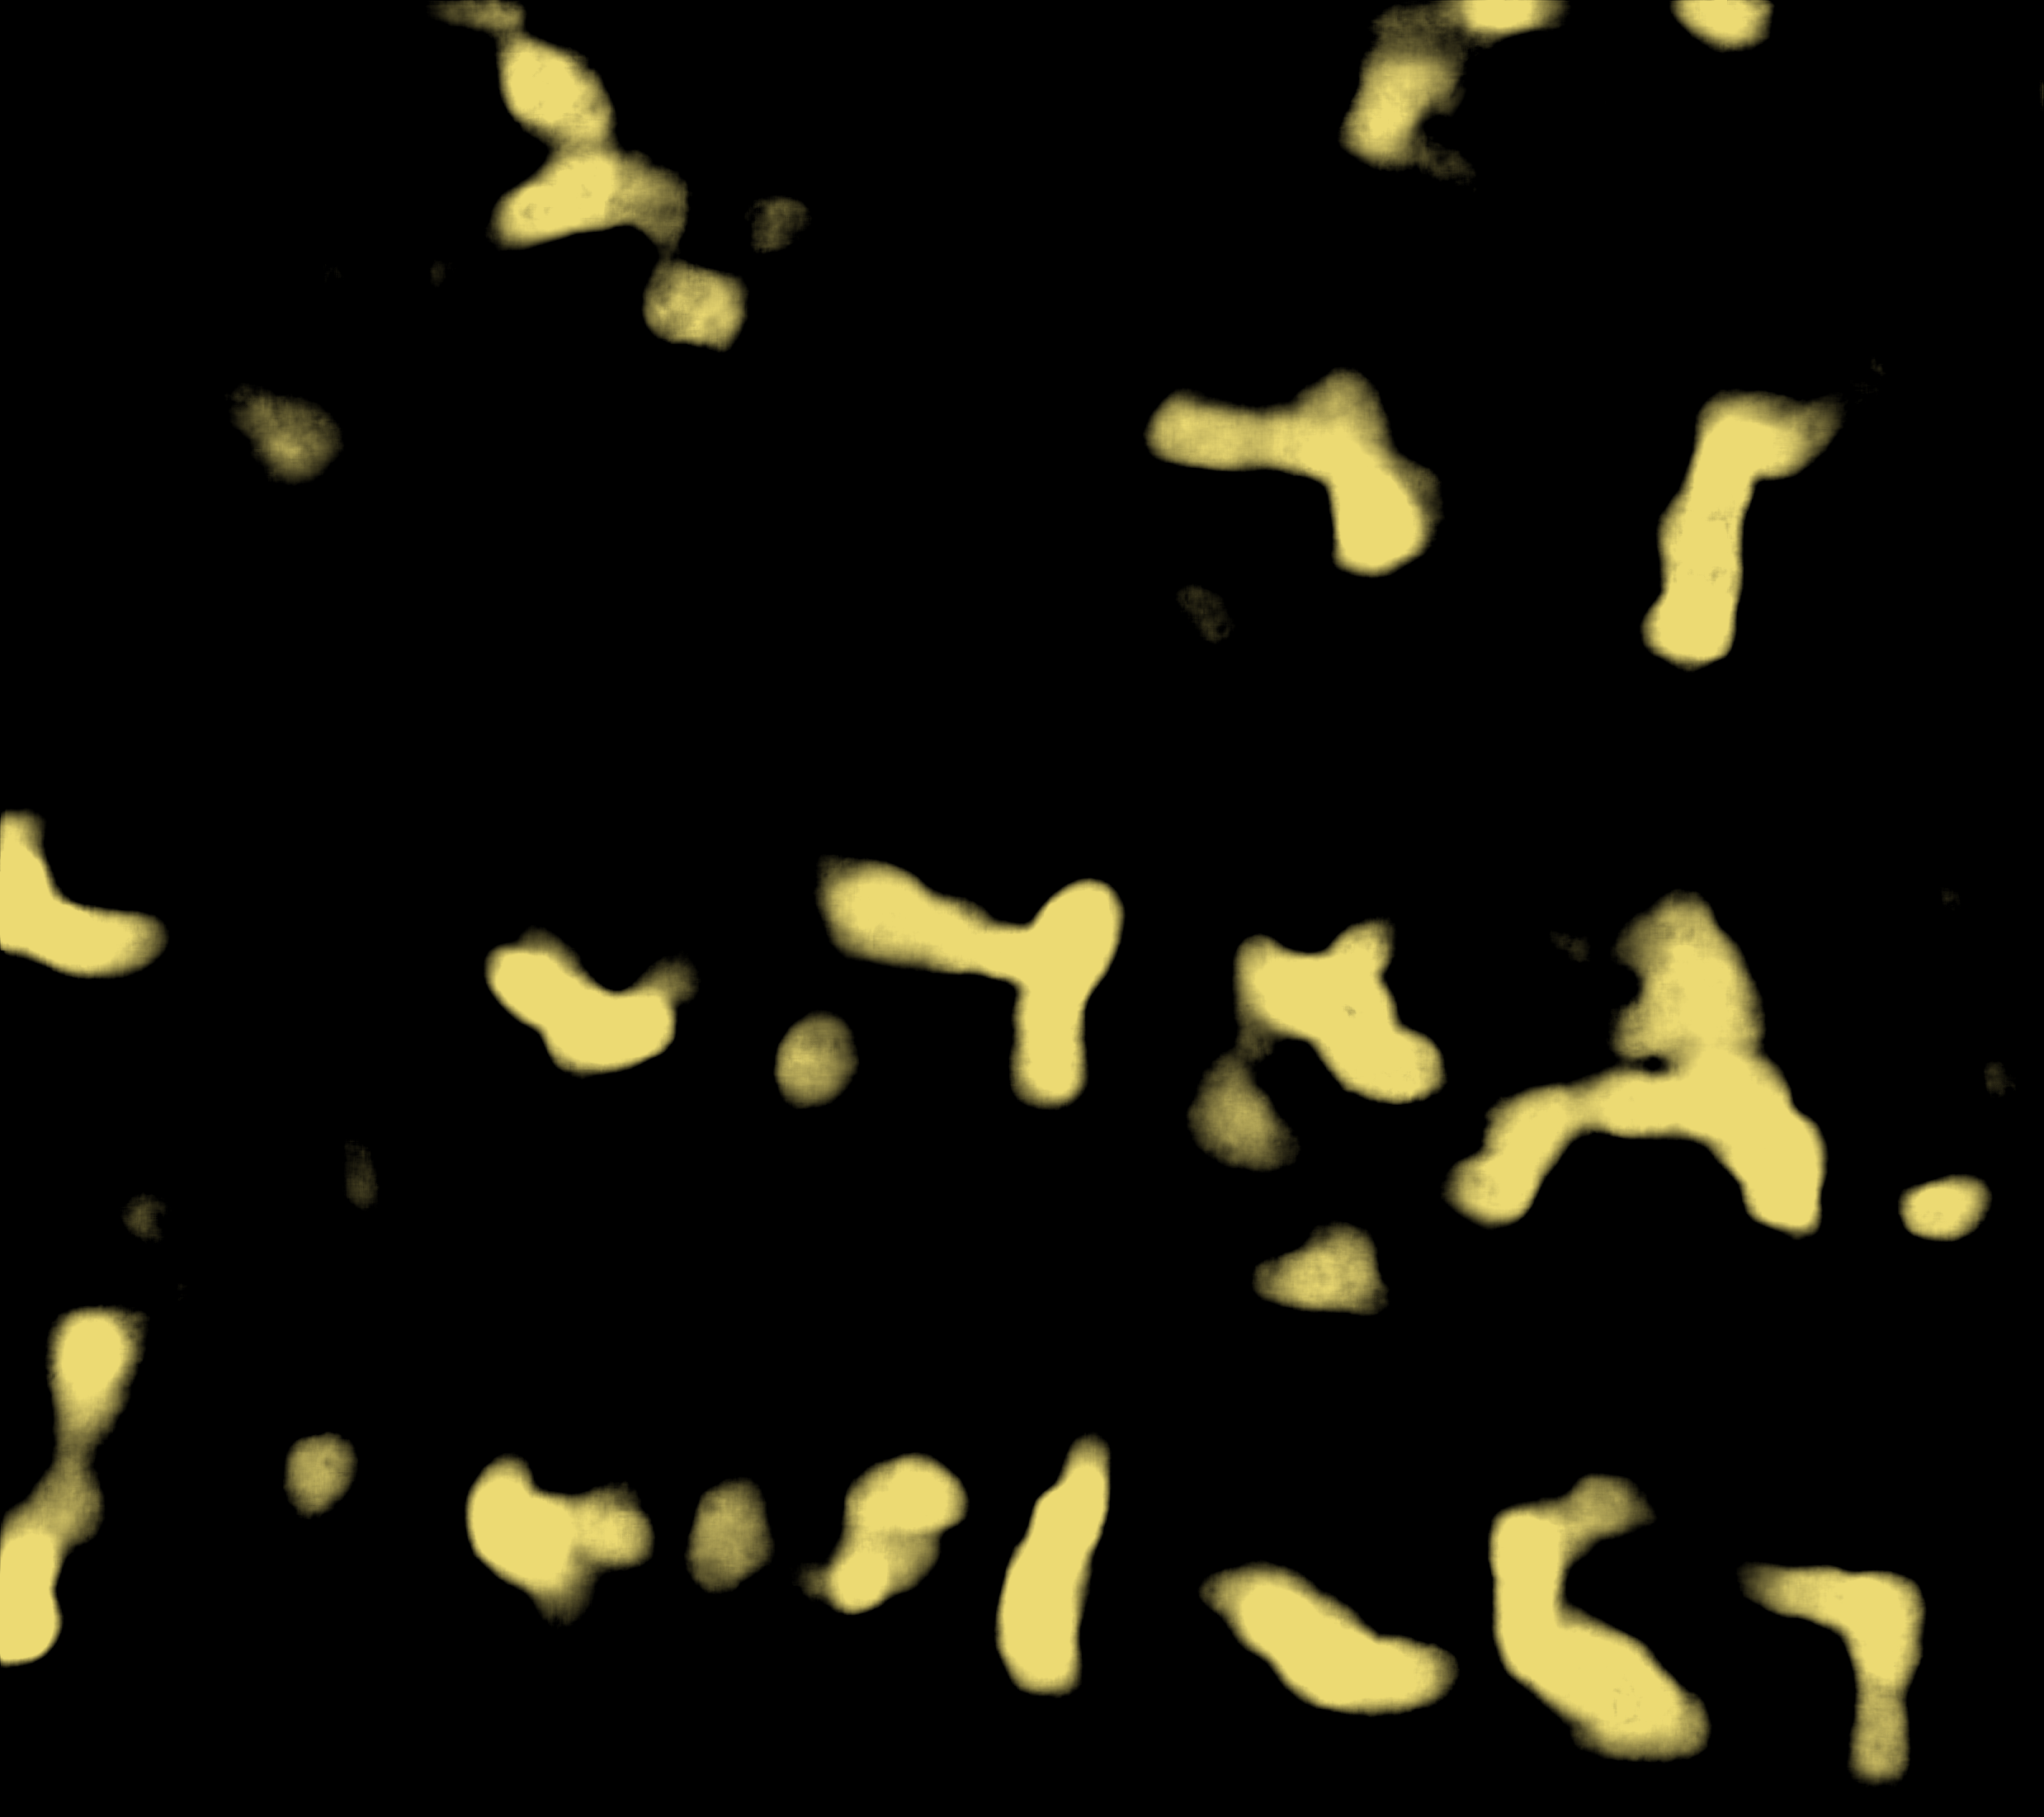
\includegraphics[width=122.48pt]{../figures/ag2/ag2_6_rectina-m2.png}}\end{minipage}}
\caption{Control unit 0841 ag2, three rows of two panels. Row 1: left, Texture; right, Labels. Row 2: left, Reader v2; right, Rectina m1 (display windows: Reader v2 0.404870 to 0.589240 (ramp); Rectina m1 0.560881 to 0.723274 (ramp)). Row 3: left, Reader v3; right, Rectina m2 (display windows: Reader v3 0.431564 to 0.660926 (ramp); Rectina m2 0.615411 to 0.768217 (ramp)). Each map is stretched between its own percentiles. Reader and model stand side by side in the rows 2 and 3.}
\end{figure}

\begin{figure}[!tbp]
\centering
\noindent\makebox[\columnwidth][c]{\begin{minipage}[t]{122.48pt}\centering\href{https://raw.githubusercontent.com/evilaliv3/vesuvius-challenge-pipeline/main/results/db27c806-rectina/src/figures/w00/w00_1_texture.png}{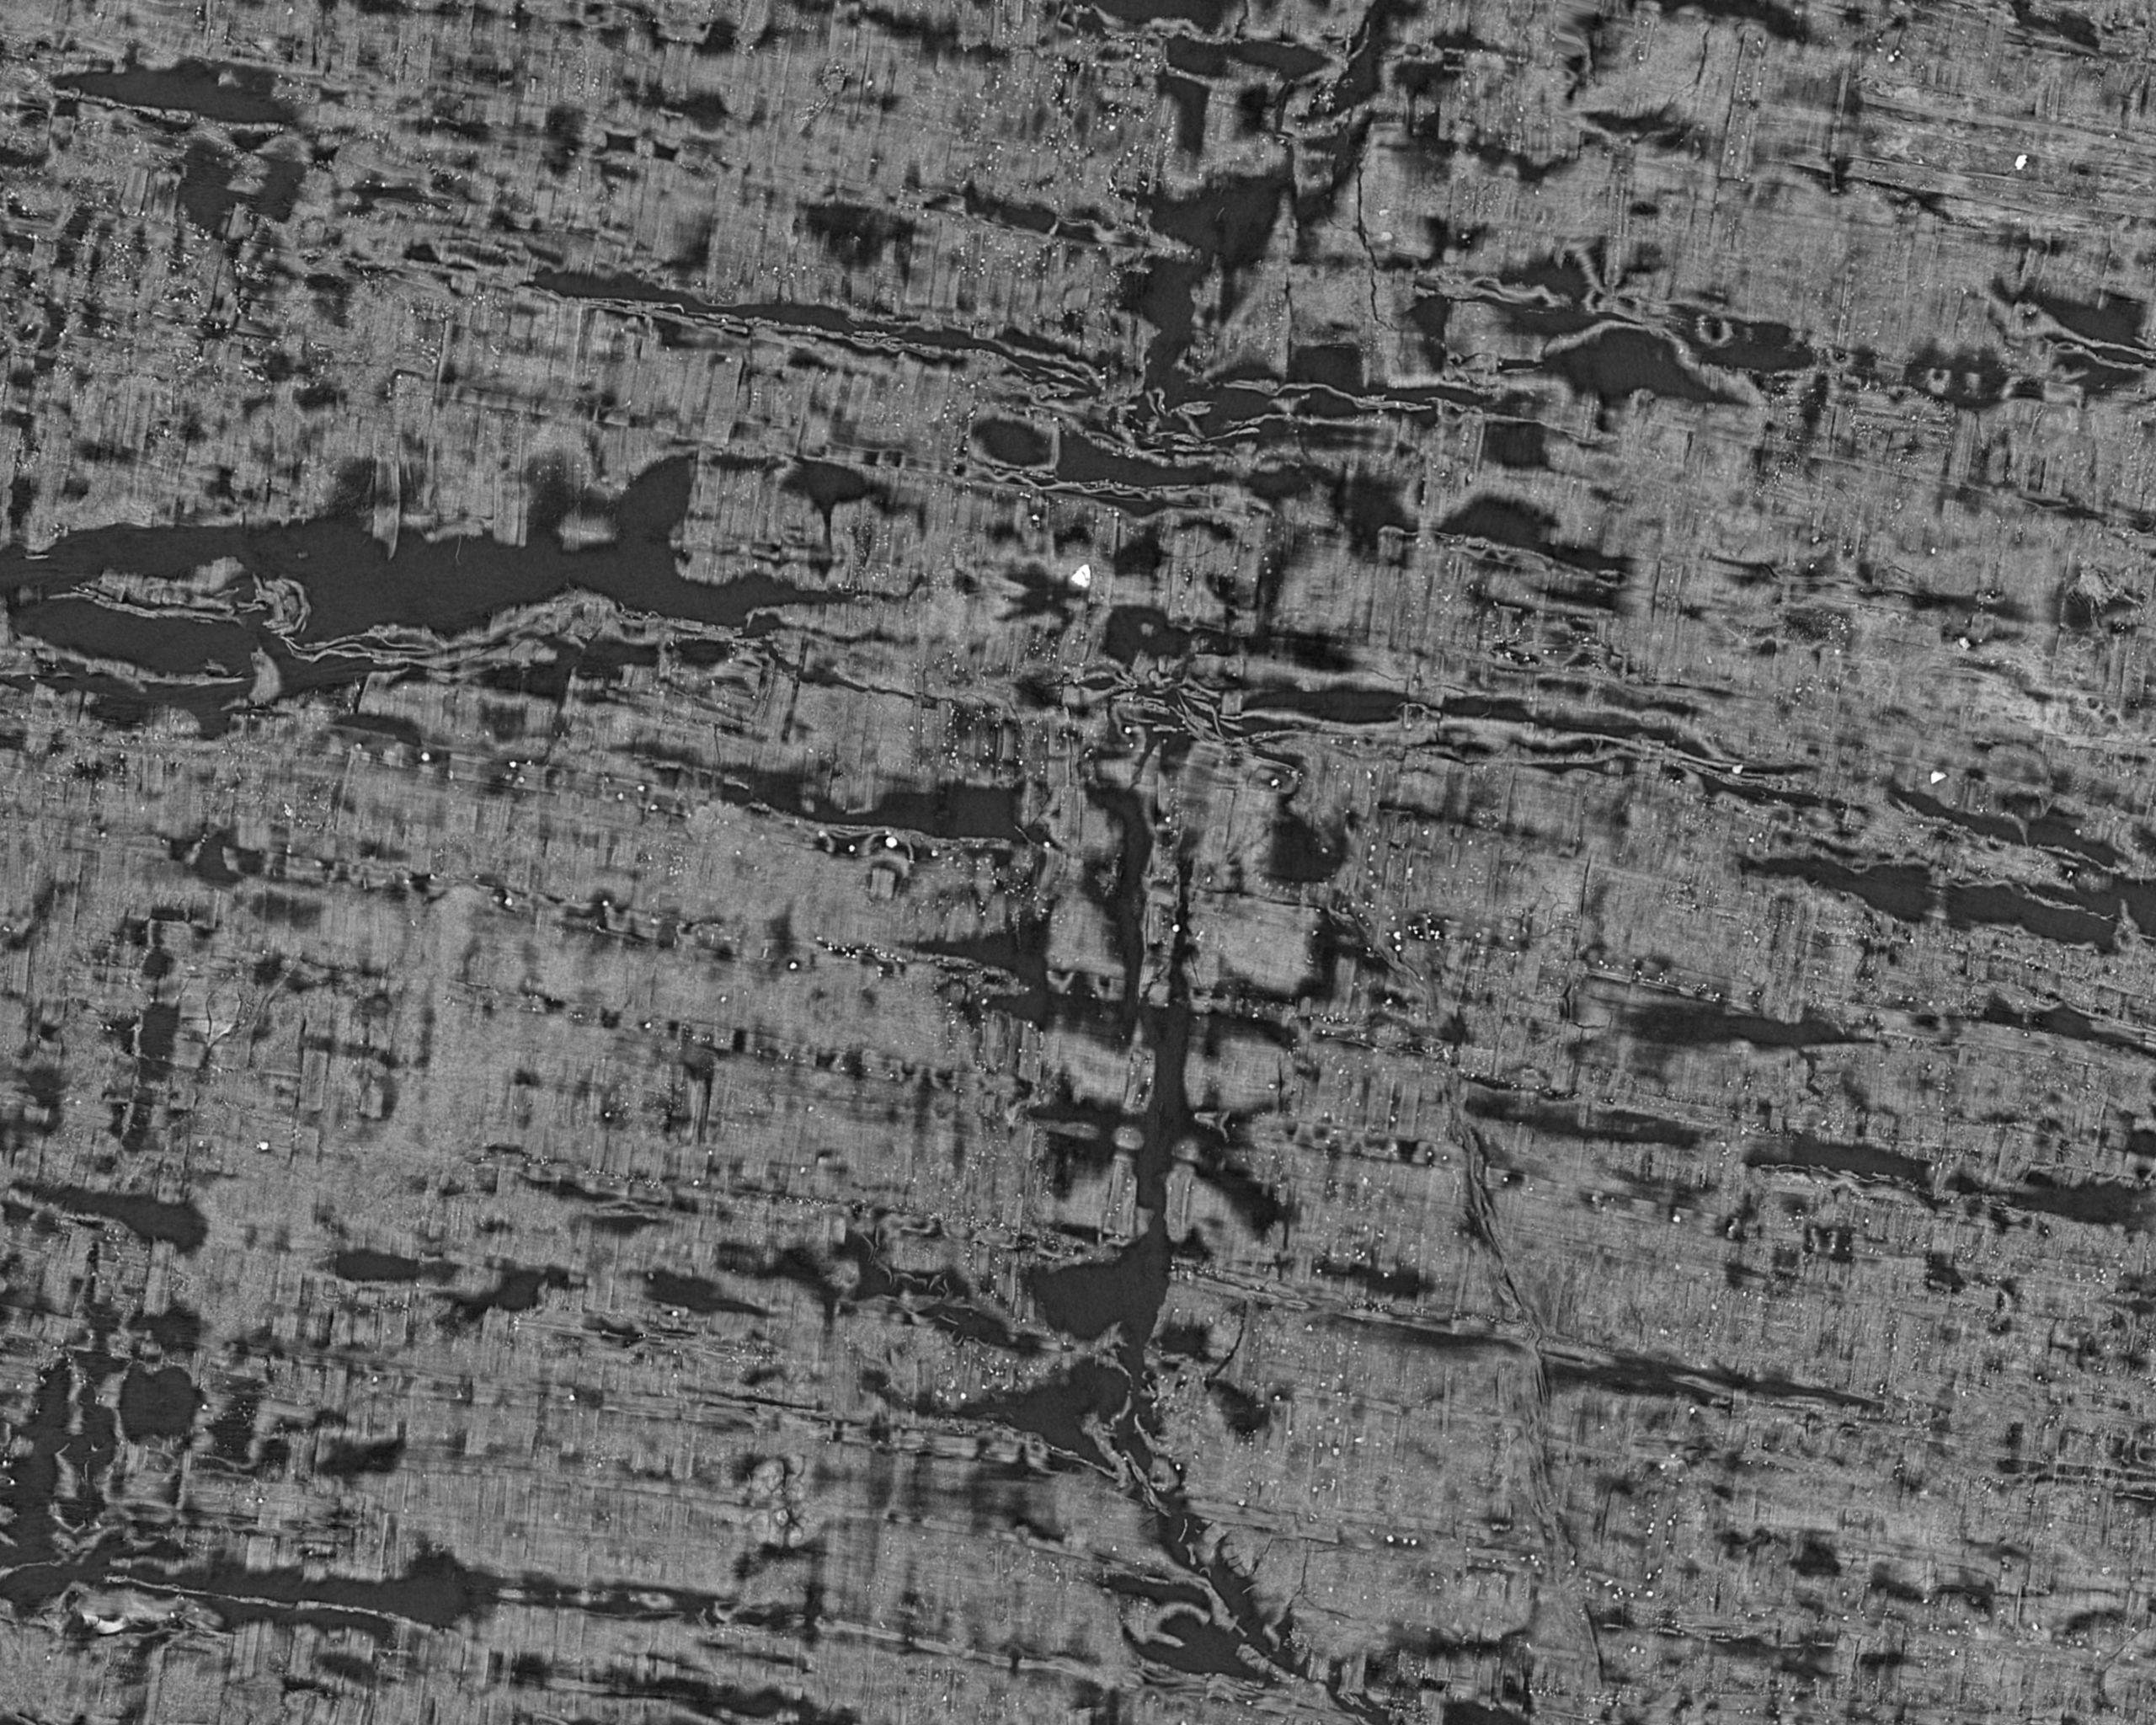
\includegraphics[width=122.48pt]{../figures/w00/w00_1_texture.png}}\end{minipage}\hspace{2pt}\begin{minipage}[t]{122.48pt}\centering\href{https://raw.githubusercontent.com/evilaliv3/vesuvius-challenge-pipeline/main/results/db27c806-rectina/src/figures/w00/w00_2_labels.png}{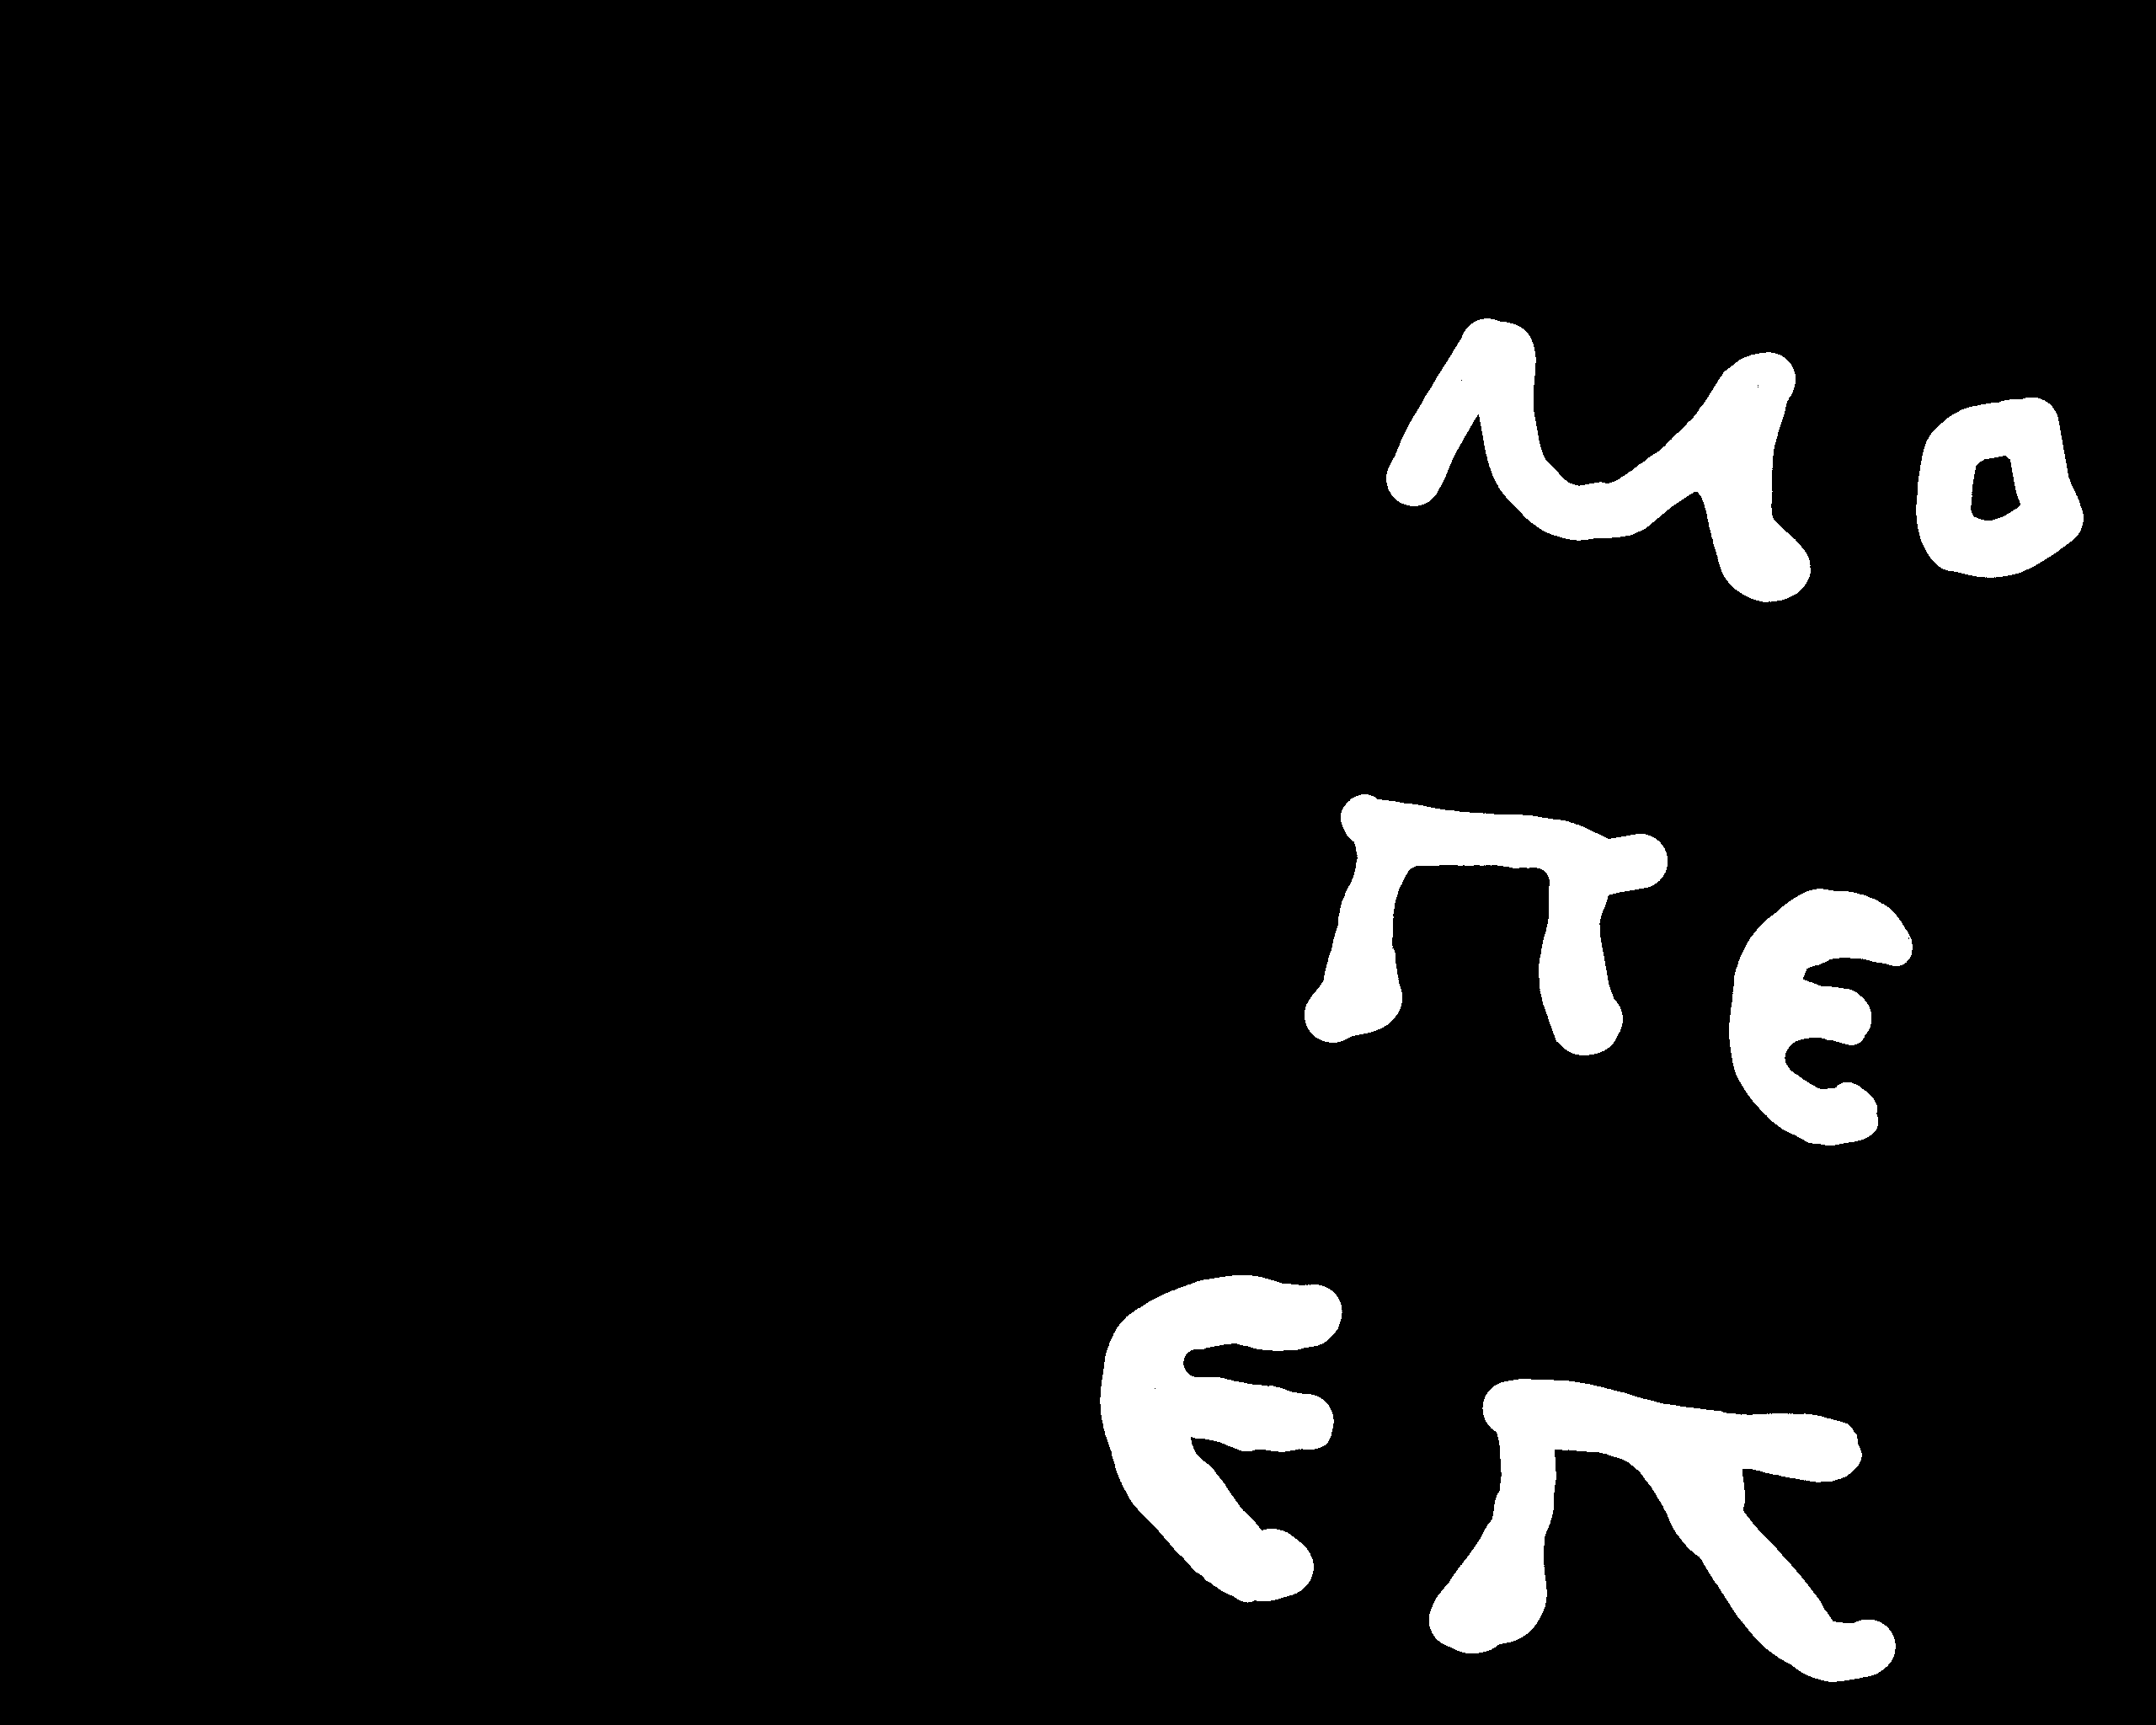
\includegraphics[width=122.48pt]{../figures/w00/w00_2_labels.png}}\end{minipage}}
\par\vspace{4pt}
\noindent\makebox[\columnwidth][c]{\begin{minipage}[t]{122.48pt}\centering\href{https://raw.githubusercontent.com/evilaliv3/vesuvius-challenge-pipeline/main/results/db27c806-rectina/src/figures/w00/w00_3_reader-v2.png}{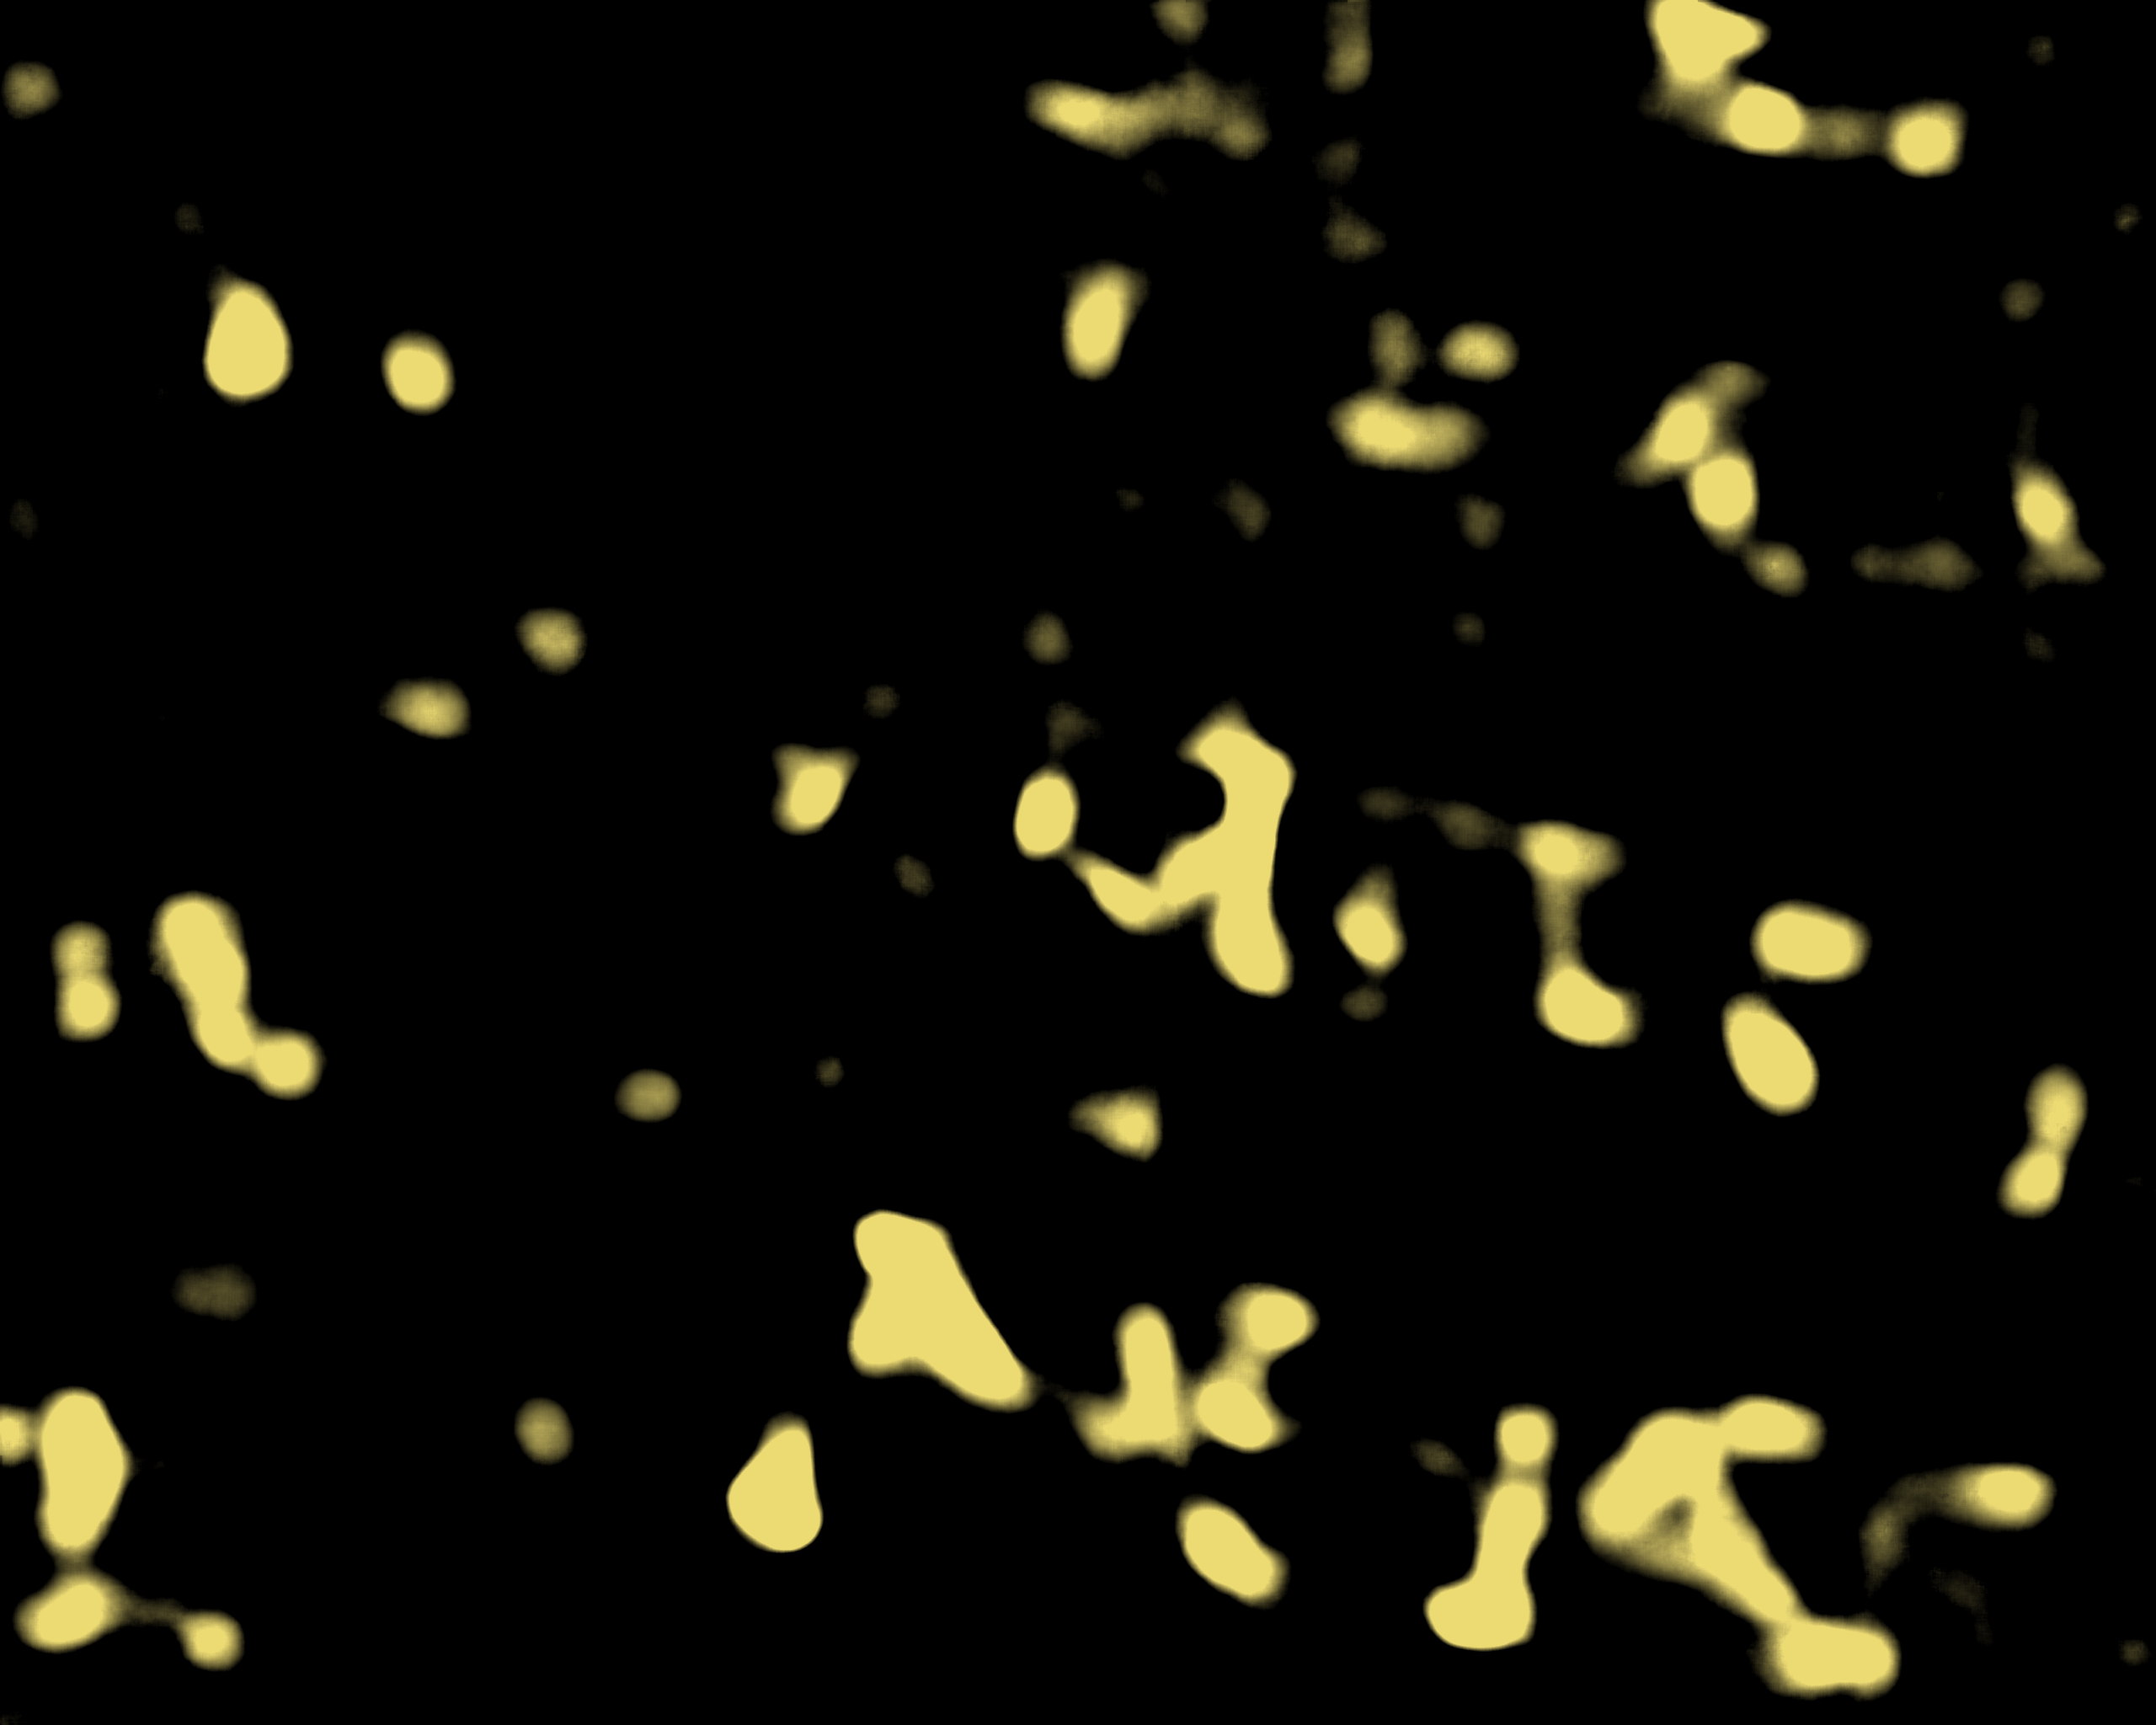
\includegraphics[width=122.48pt]{../figures/w00/w00_3_reader-v2.png}}\end{minipage}\hspace{2pt}\begin{minipage}[t]{122.48pt}\centering\href{https://raw.githubusercontent.com/evilaliv3/vesuvius-challenge-pipeline/main/results/db27c806-rectina/src/figures/w00/w00_5_rectina-m1.png}{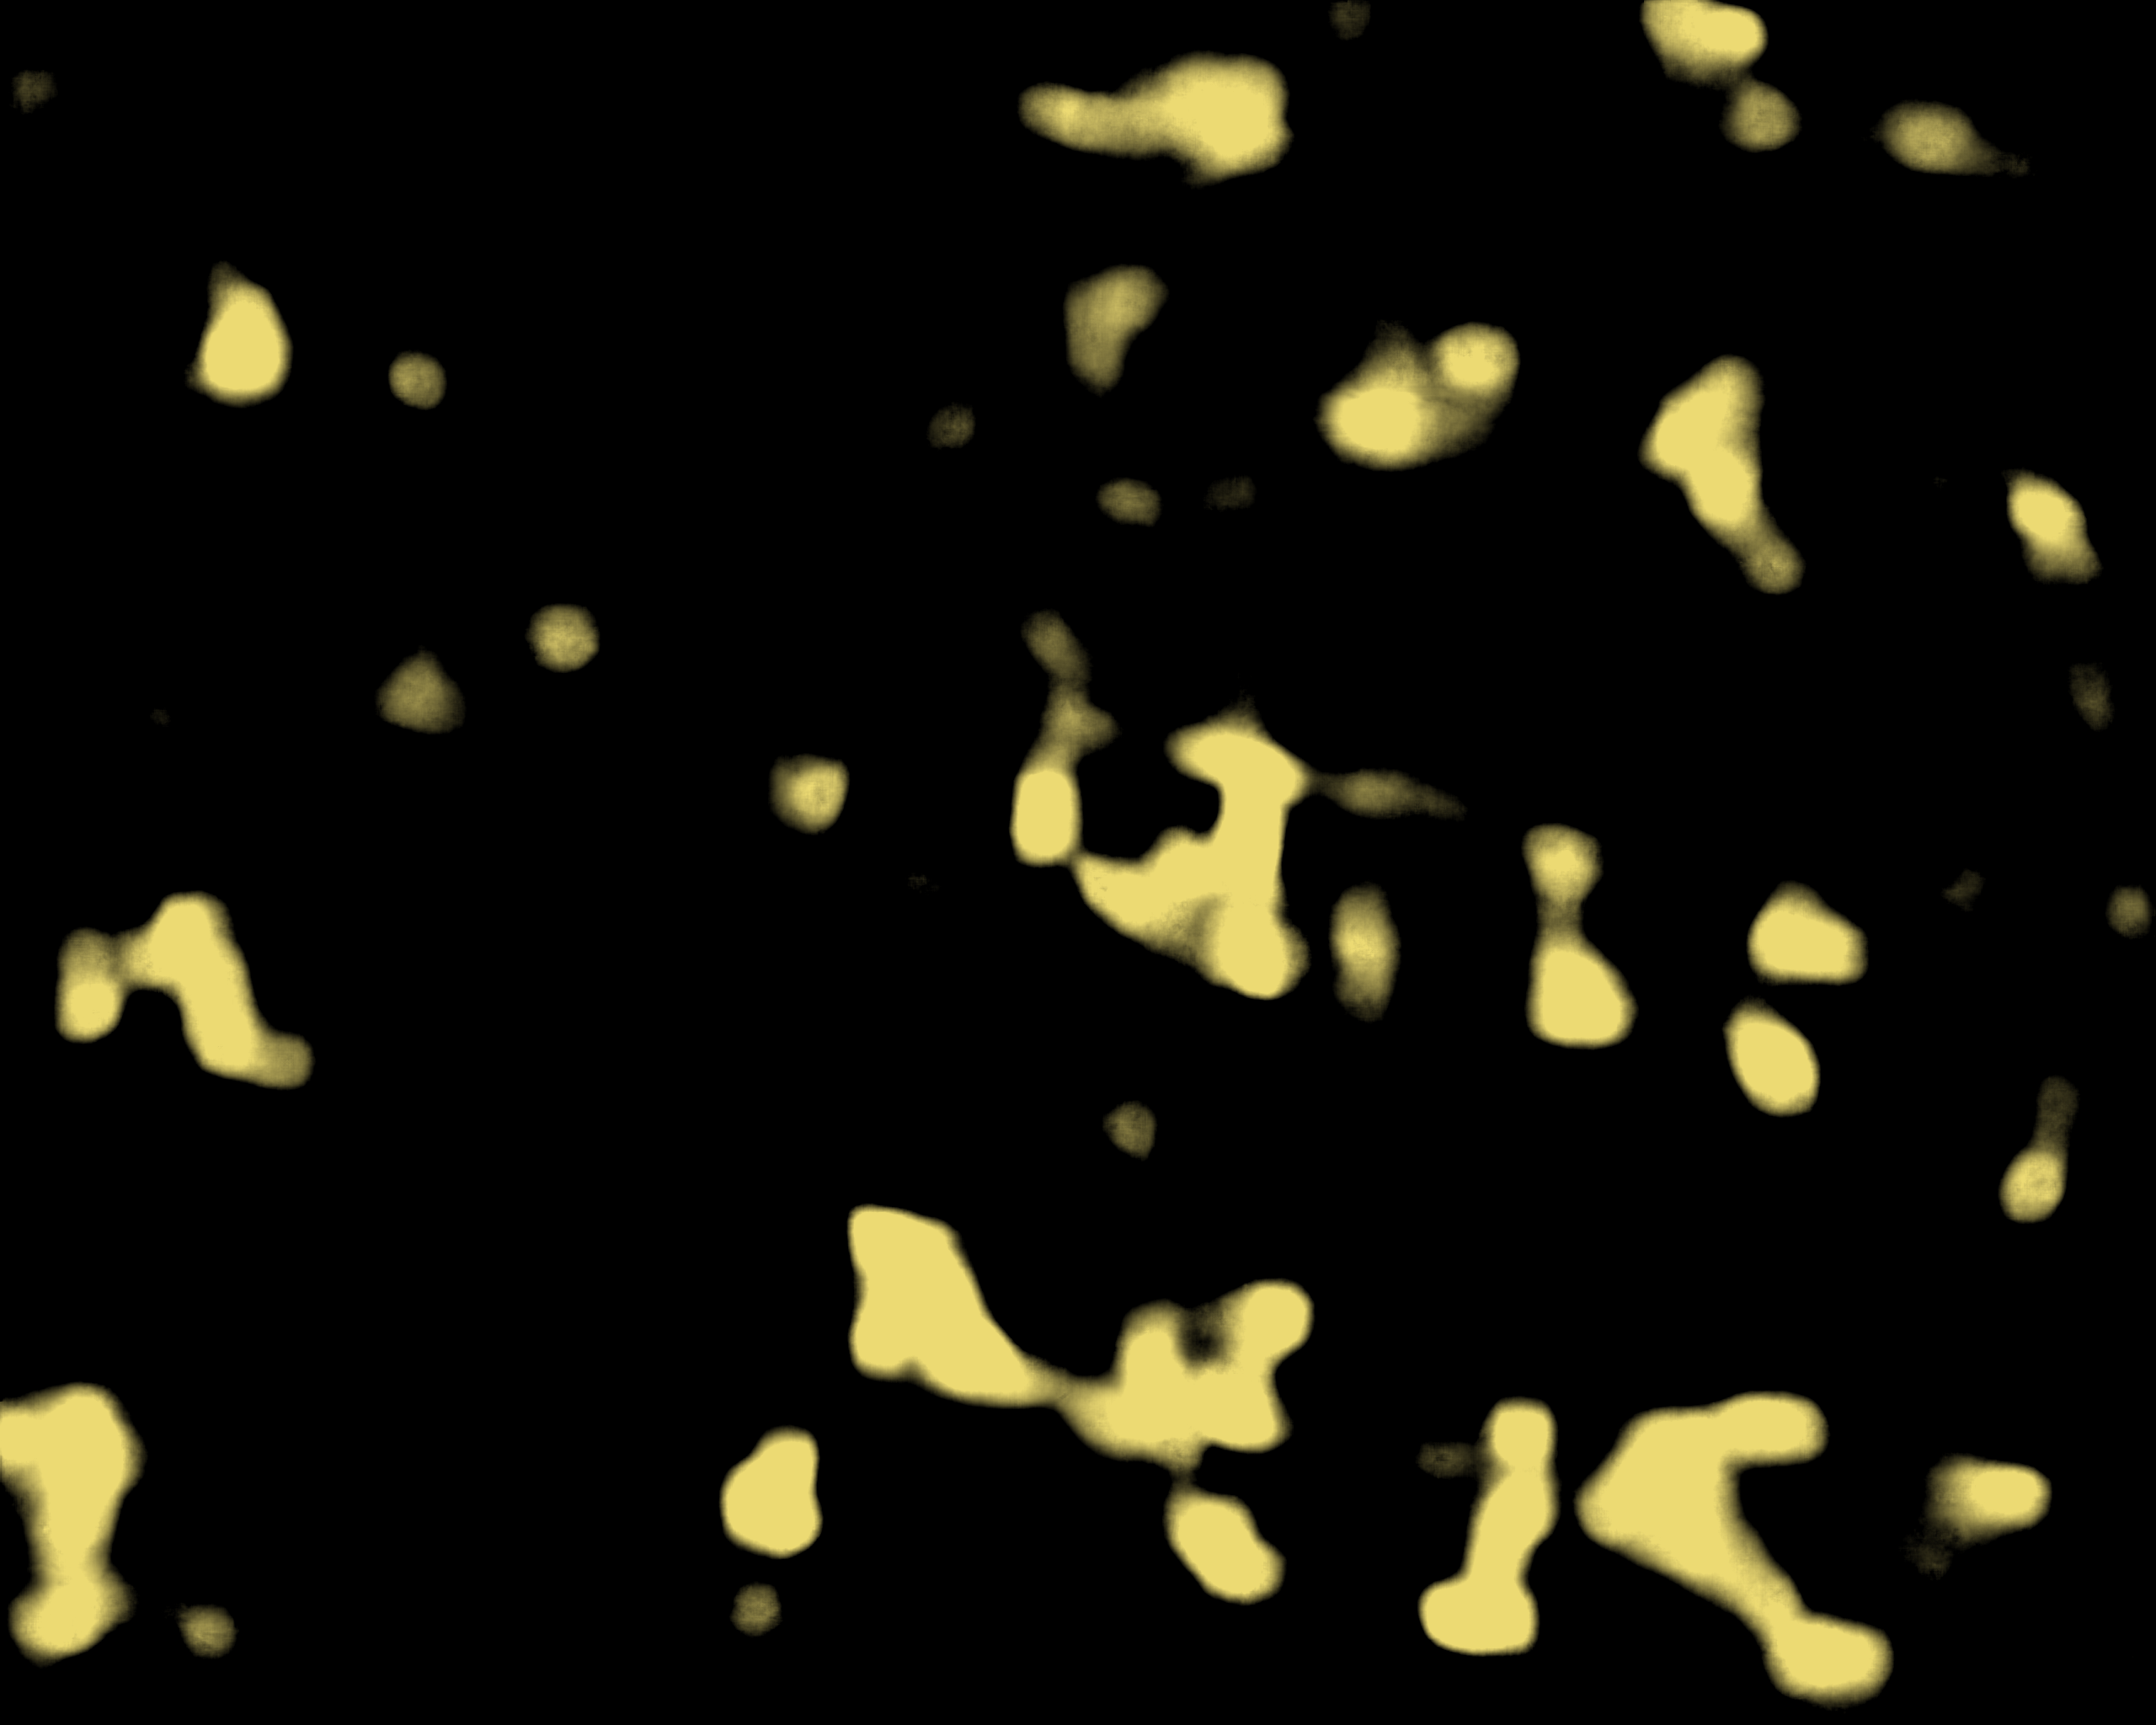
\includegraphics[width=122.48pt]{../figures/w00/w00_5_rectina-m1.png}}\end{minipage}}
\par\vspace{4pt}
\noindent\makebox[\columnwidth][c]{\begin{minipage}[t]{122.48pt}\centering\href{https://raw.githubusercontent.com/evilaliv3/vesuvius-challenge-pipeline/main/results/db27c806-rectina/src/figures/w00/w00_4_reader-v3.png}{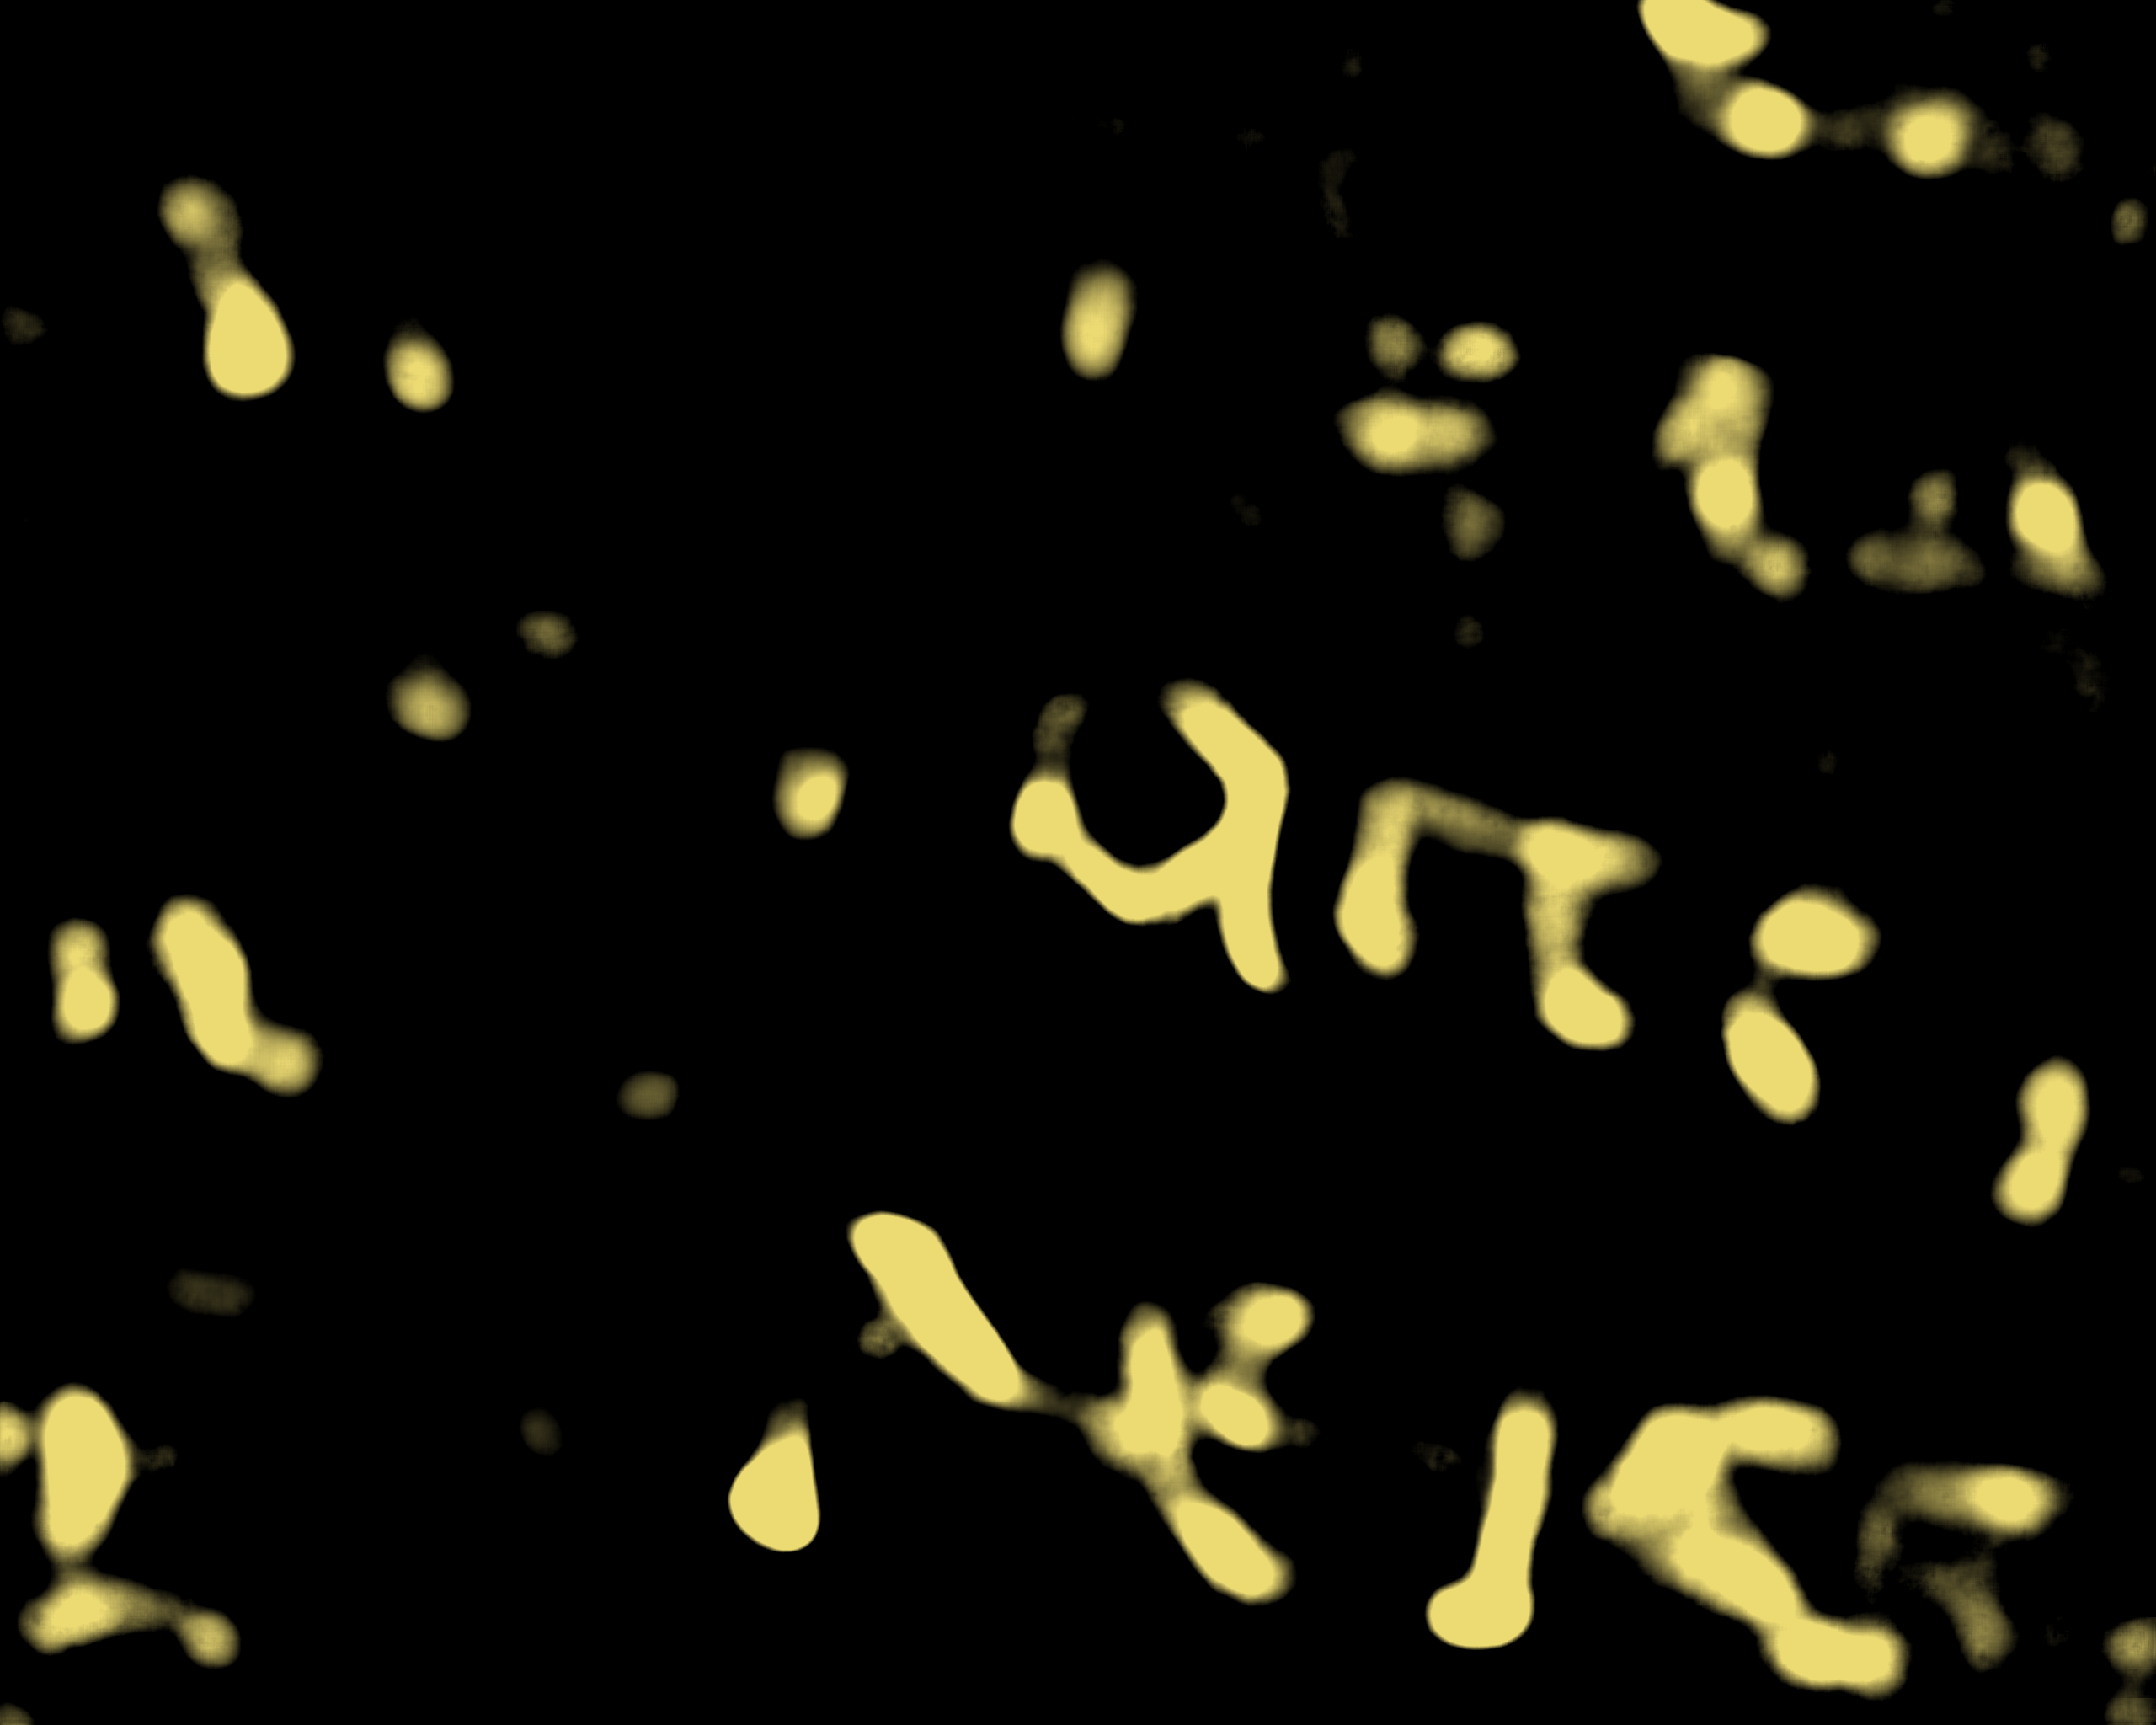
\includegraphics[width=122.48pt]{../figures/w00/w00_4_reader-v3.png}}\end{minipage}\hspace{2pt}\begin{minipage}[t]{122.48pt}\centering\href{https://raw.githubusercontent.com/evilaliv3/vesuvius-challenge-pipeline/main/results/db27c806-rectina/src/figures/w00/w00_6_rectina-m2.png}{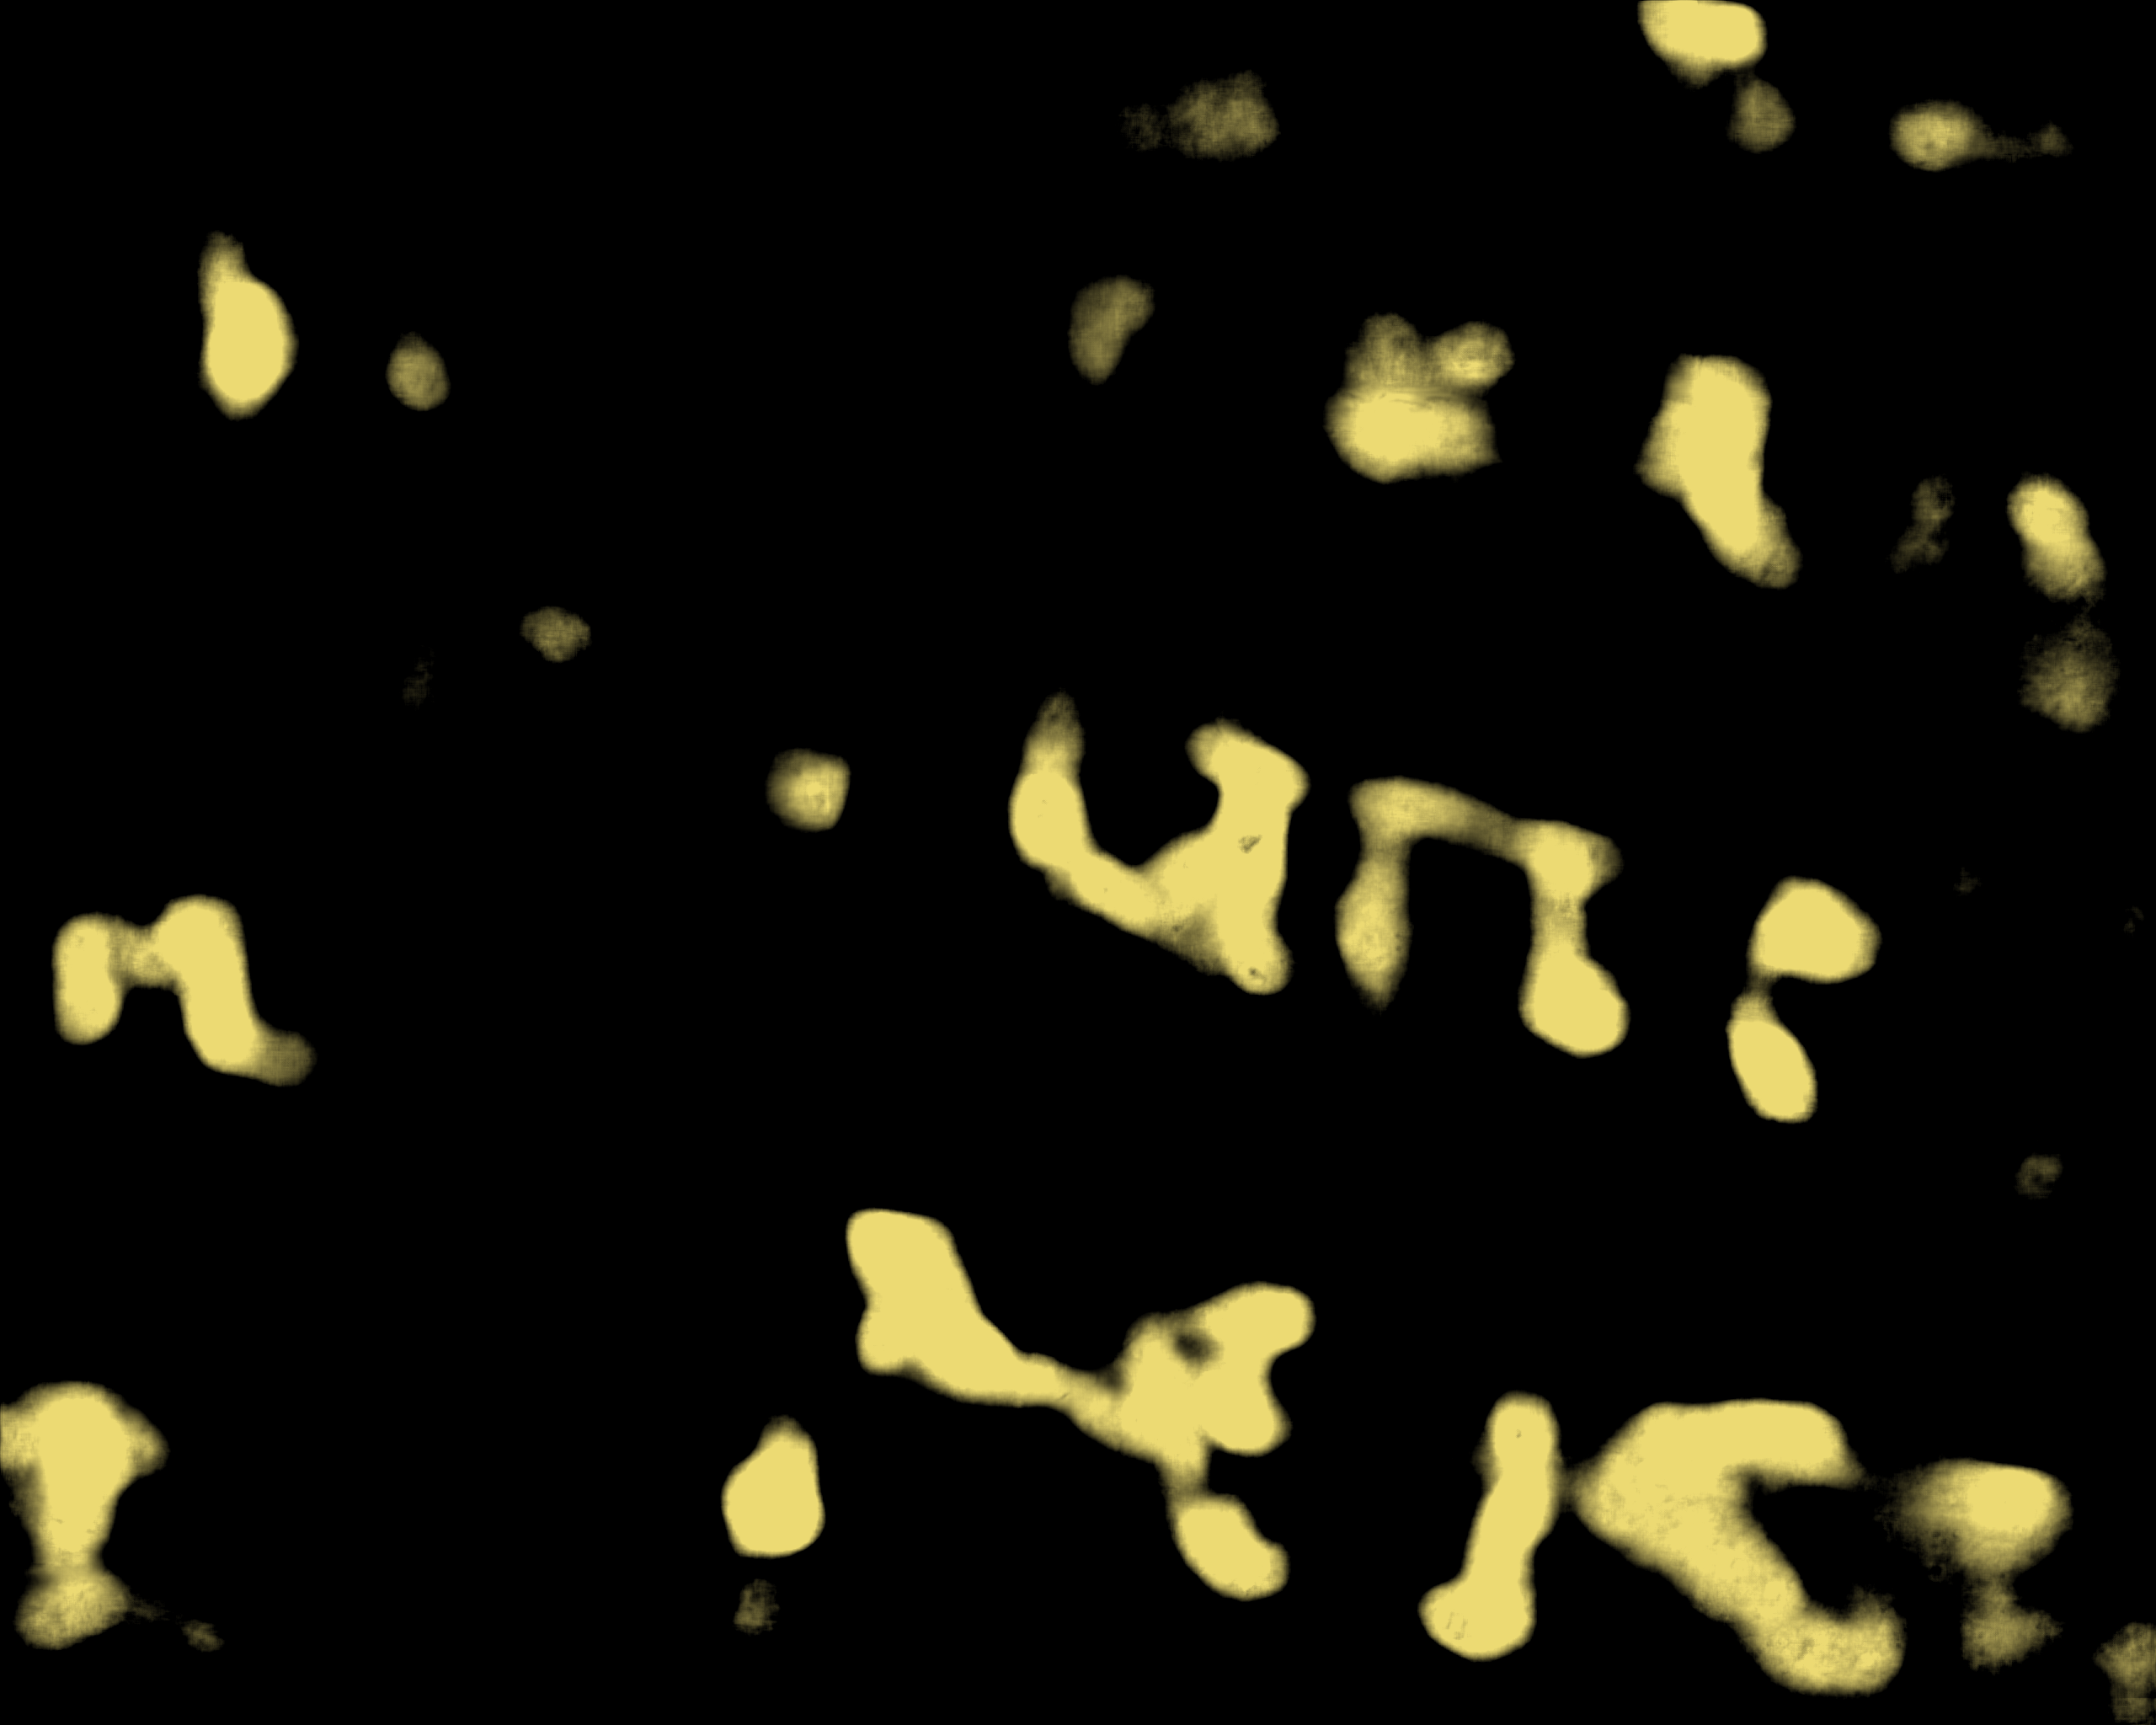
\includegraphics[width=122.48pt]{../figures/w00/w00_6_rectina-m2.png}}\end{minipage}}
\caption{Control unit 0841 w00, three rows of two panels. Row 1: left, Texture; right, Labels. Row 2: left, Reader v2; right, Rectina m1 (display windows: Reader v2 0.419276 to 0.595756 (ramp); Rectina m1 0.577431 to 0.724182 (ramp)). Row 3: left, Reader v3; right, Rectina m2 (display windows: Reader v3 0.454060 to 0.672485 (ramp); Rectina m2 0.650603 to 0.768363 (ramp)). Each map is stretched between its own percentiles. Reader and model stand side by side in the rows 2 and 3.}
\end{figure}

\begin{figure}[!tbp]
\centering
\noindent\makebox[\columnwidth][c]{\begin{minipage}[t]{122.48pt}\centering\href{https://raw.githubusercontent.com/evilaliv3/vesuvius-challenge-pipeline/main/results/db27c806-rectina/src/figures/0343/0343_1_texture.png}{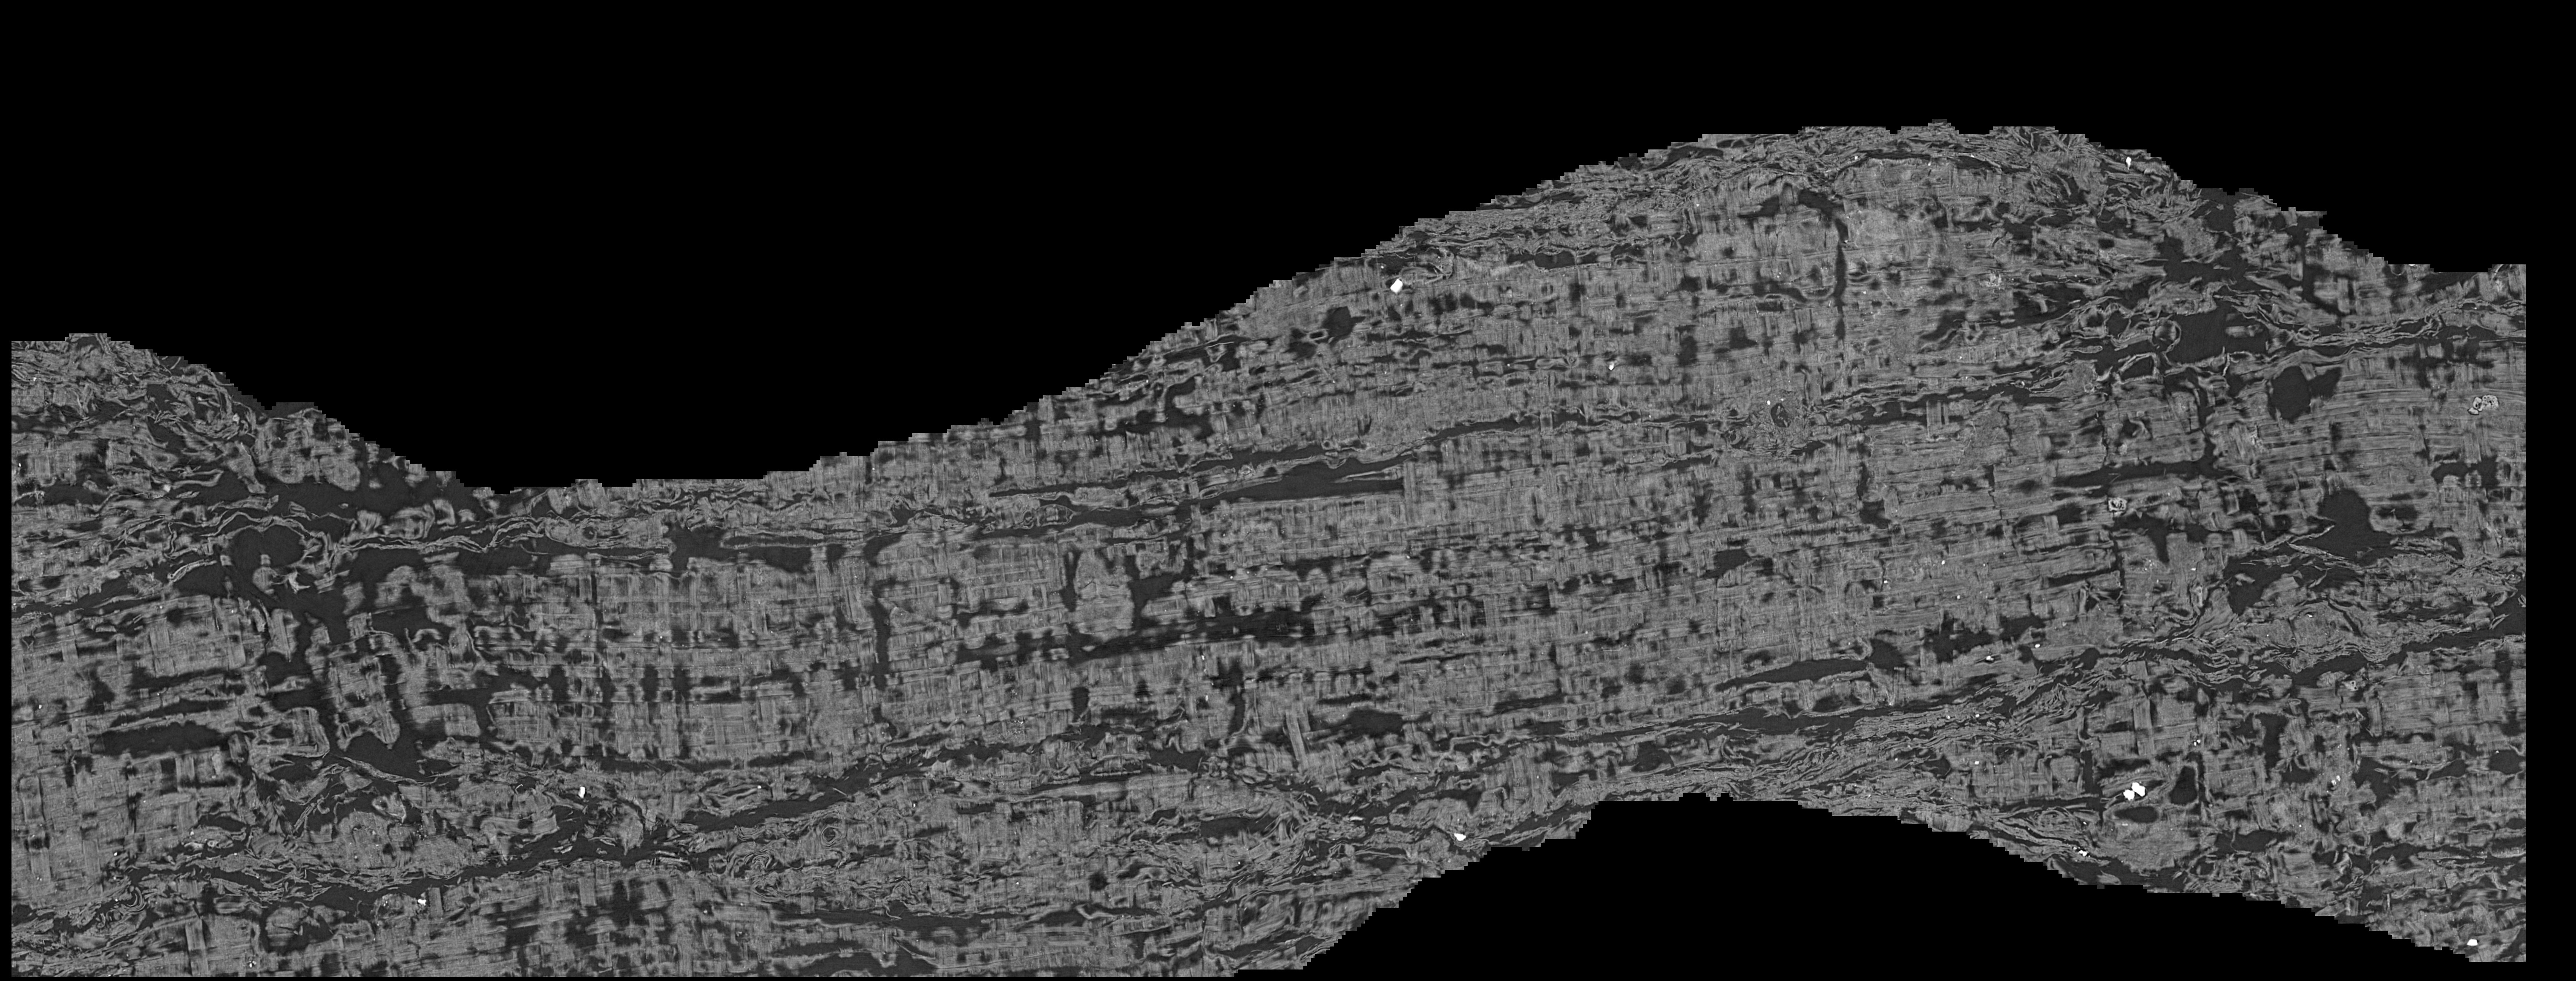
\includegraphics[width=122.48pt]{../figures/0343/0343_1_texture.png}}\end{minipage}\hspace{2pt}\begin{minipage}[t]{122.48pt}\centering\href{https://raw.githubusercontent.com/evilaliv3/vesuvius-challenge-pipeline/main/results/db27c806-rectina/src/figures/0343/0343_2_labels.png}{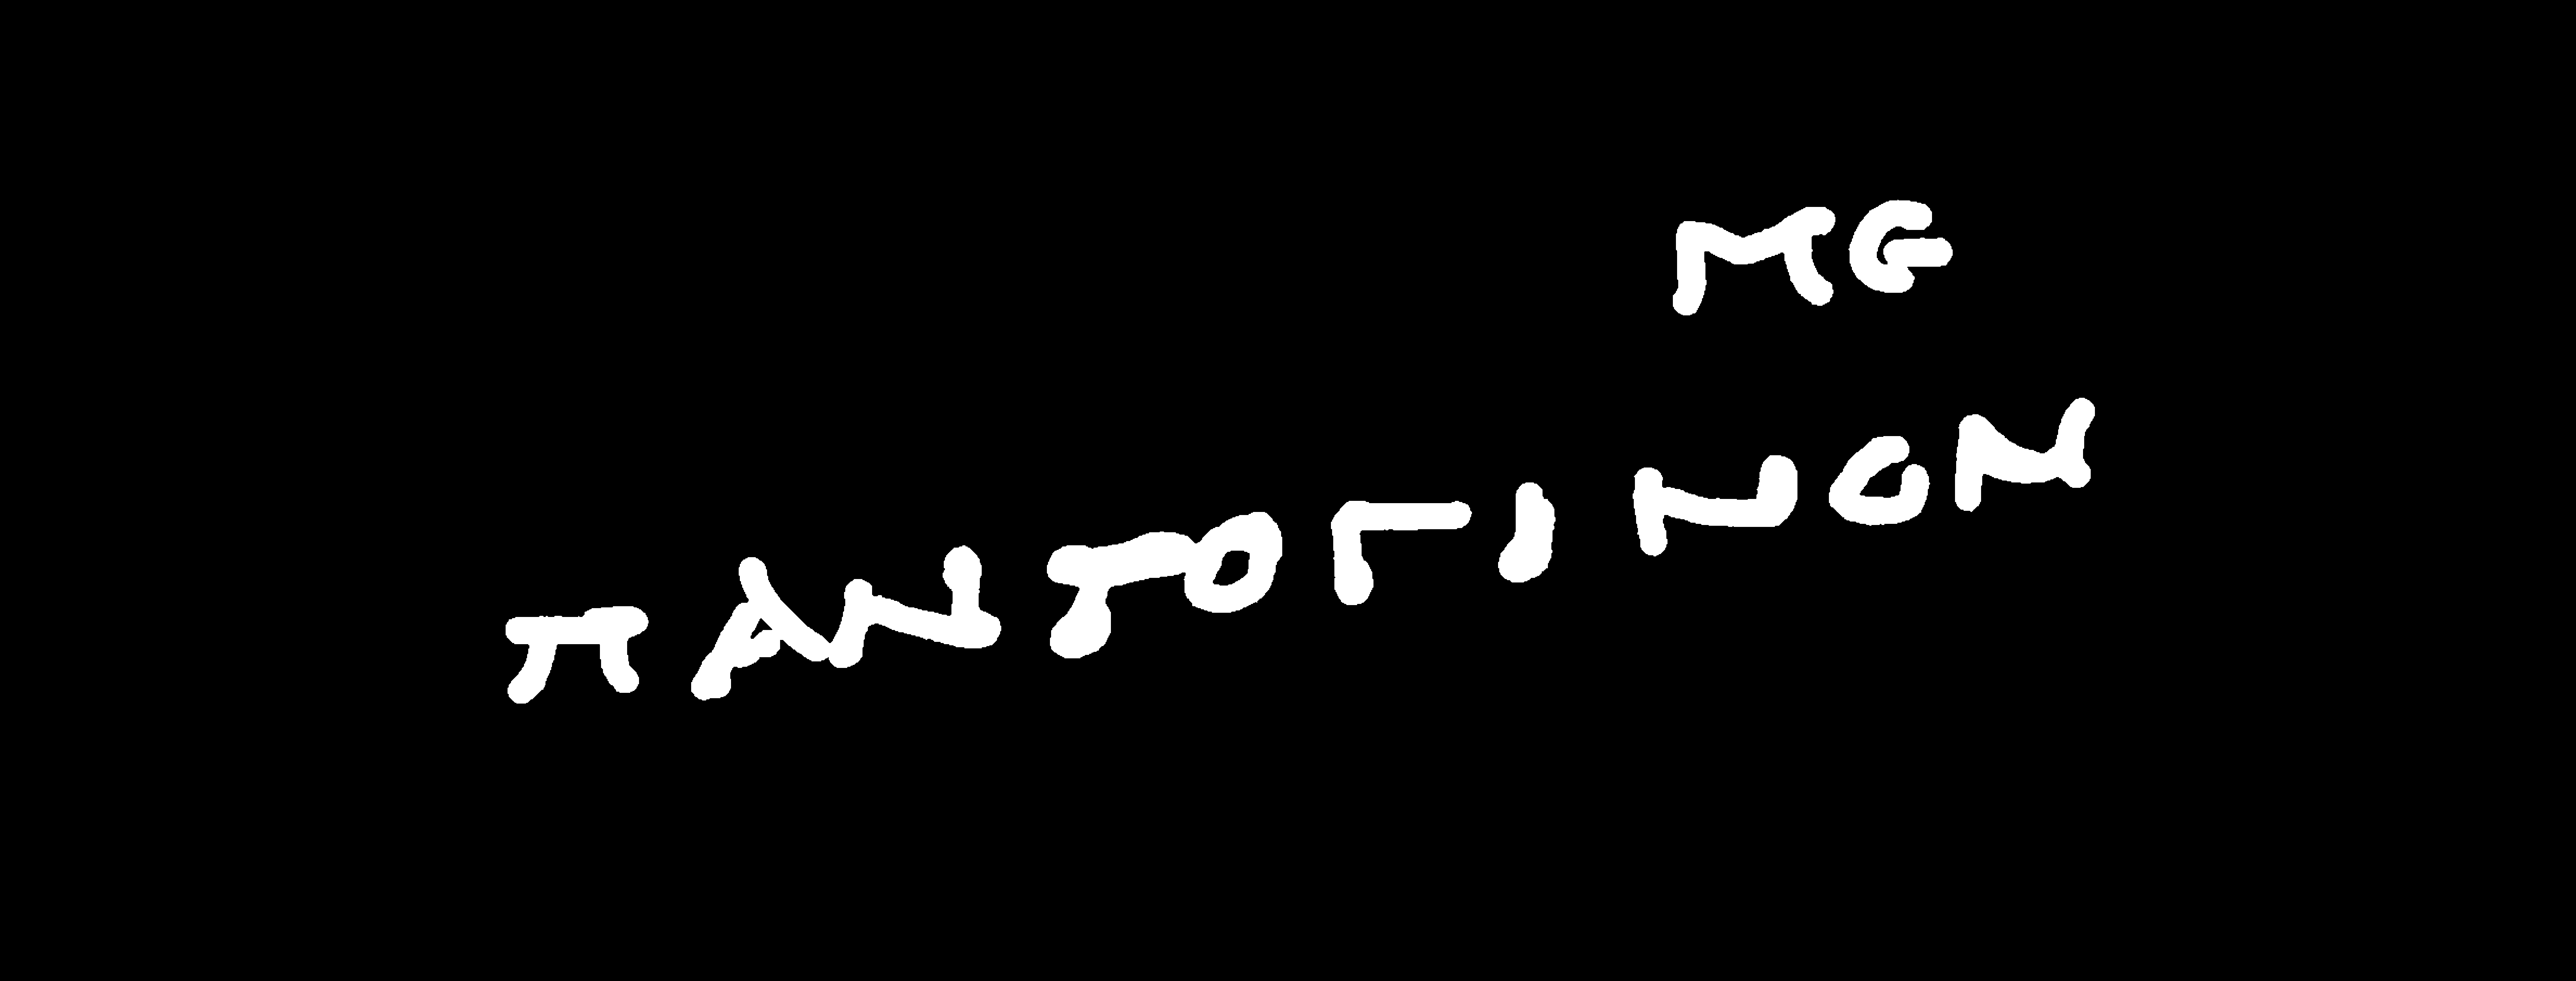
\includegraphics[width=122.48pt]{../figures/0343/0343_2_labels.png}}\end{minipage}}
\par\vspace{4pt}
\noindent\makebox[\columnwidth][c]{\begin{minipage}[t]{122.48pt}\centering\href{https://raw.githubusercontent.com/evilaliv3/vesuvius-challenge-pipeline/main/results/db27c806-rectina/src/figures/0343/0343_3_reader-v2.png}{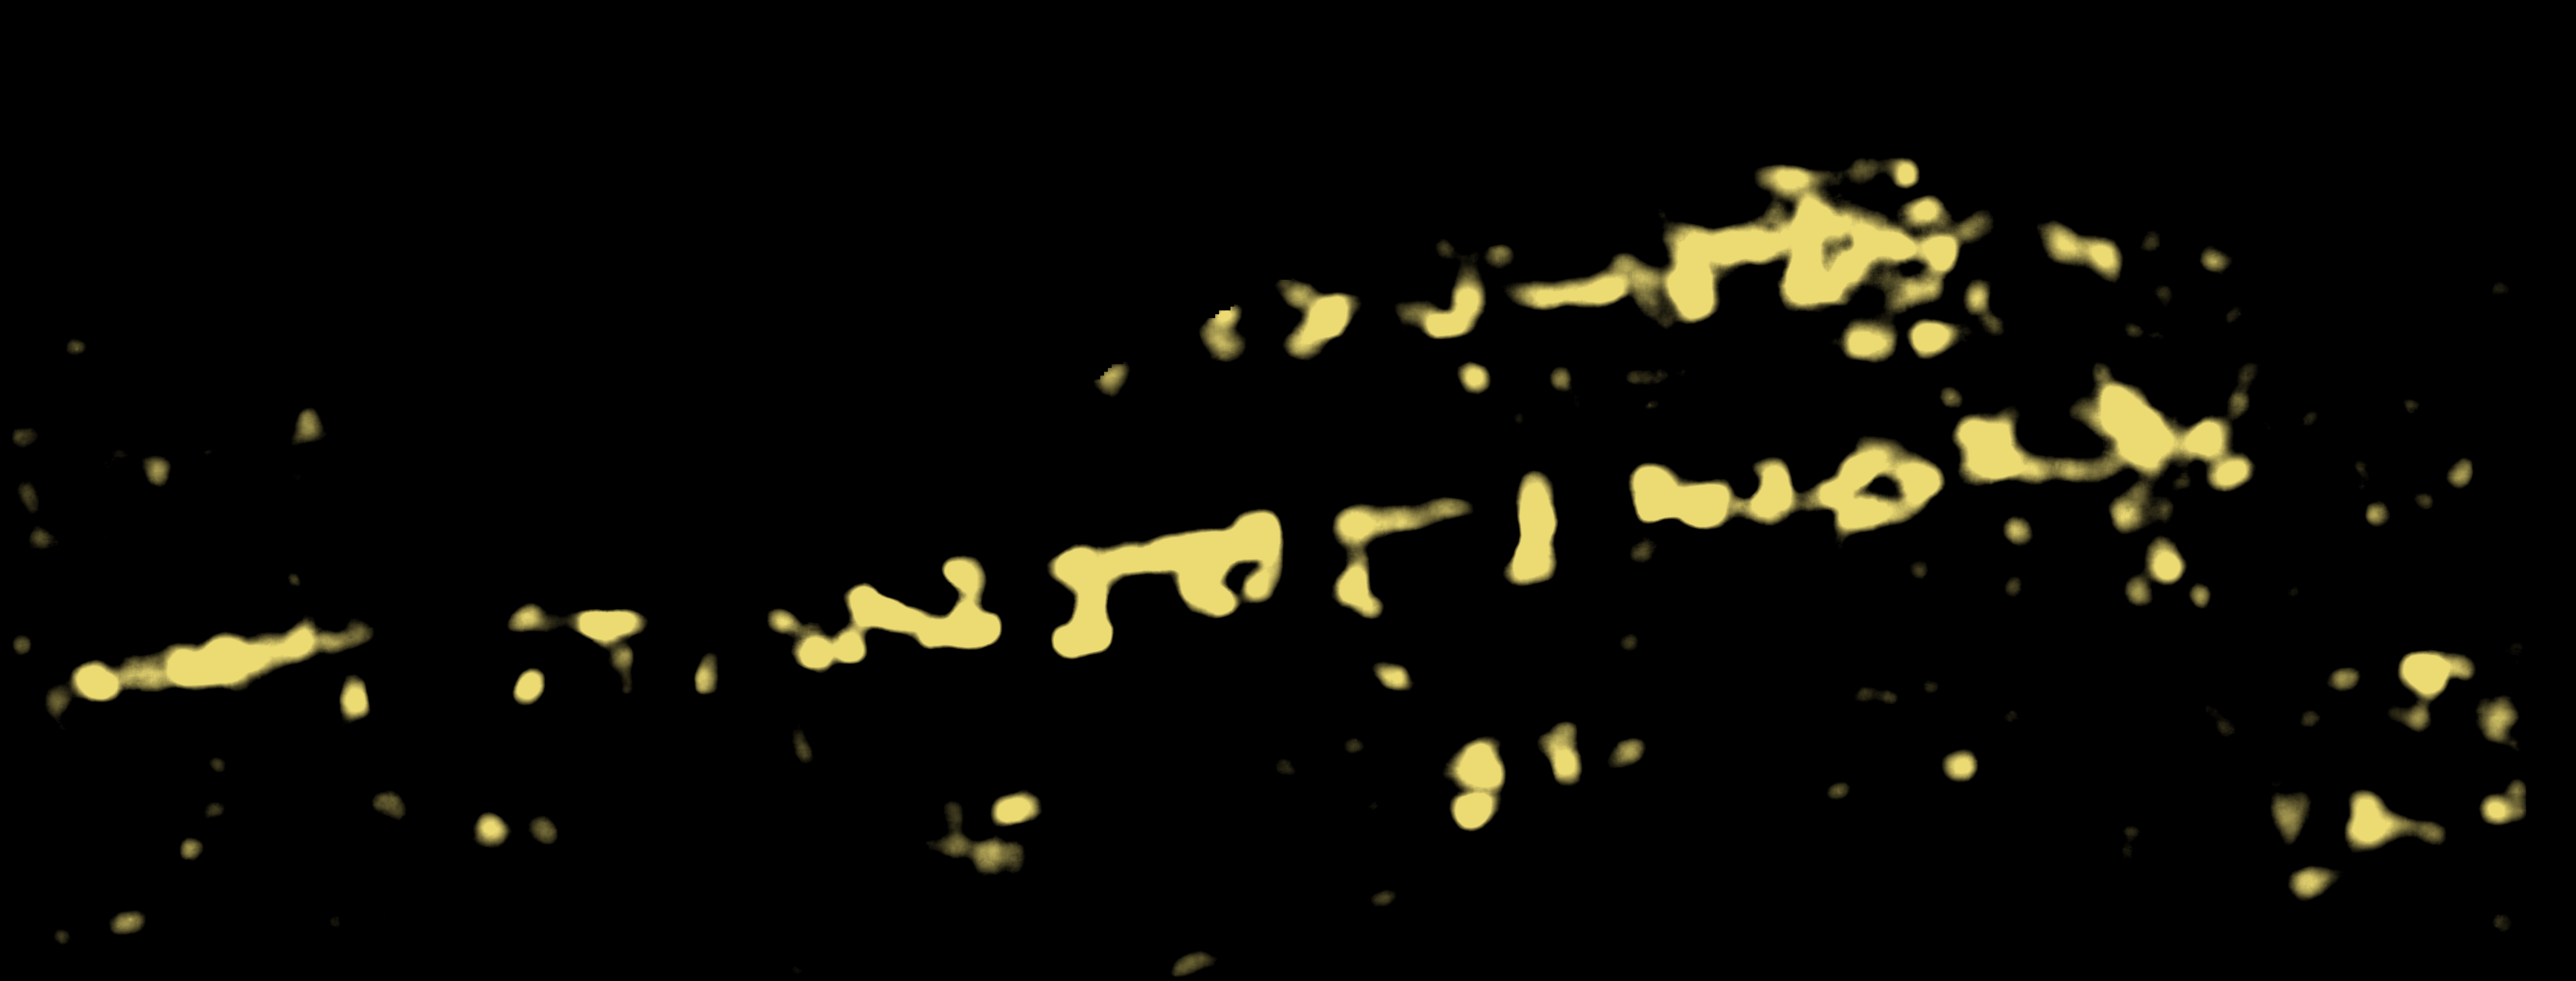
\includegraphics[width=122.48pt]{../figures/0343/0343_3_reader-v2.png}}\end{minipage}\hspace{2pt}\begin{minipage}[t]{122.48pt}\centering\href{https://raw.githubusercontent.com/evilaliv3/vesuvius-challenge-pipeline/main/results/db27c806-rectina/src/figures/0343/0343_5_rectina-m1.png}{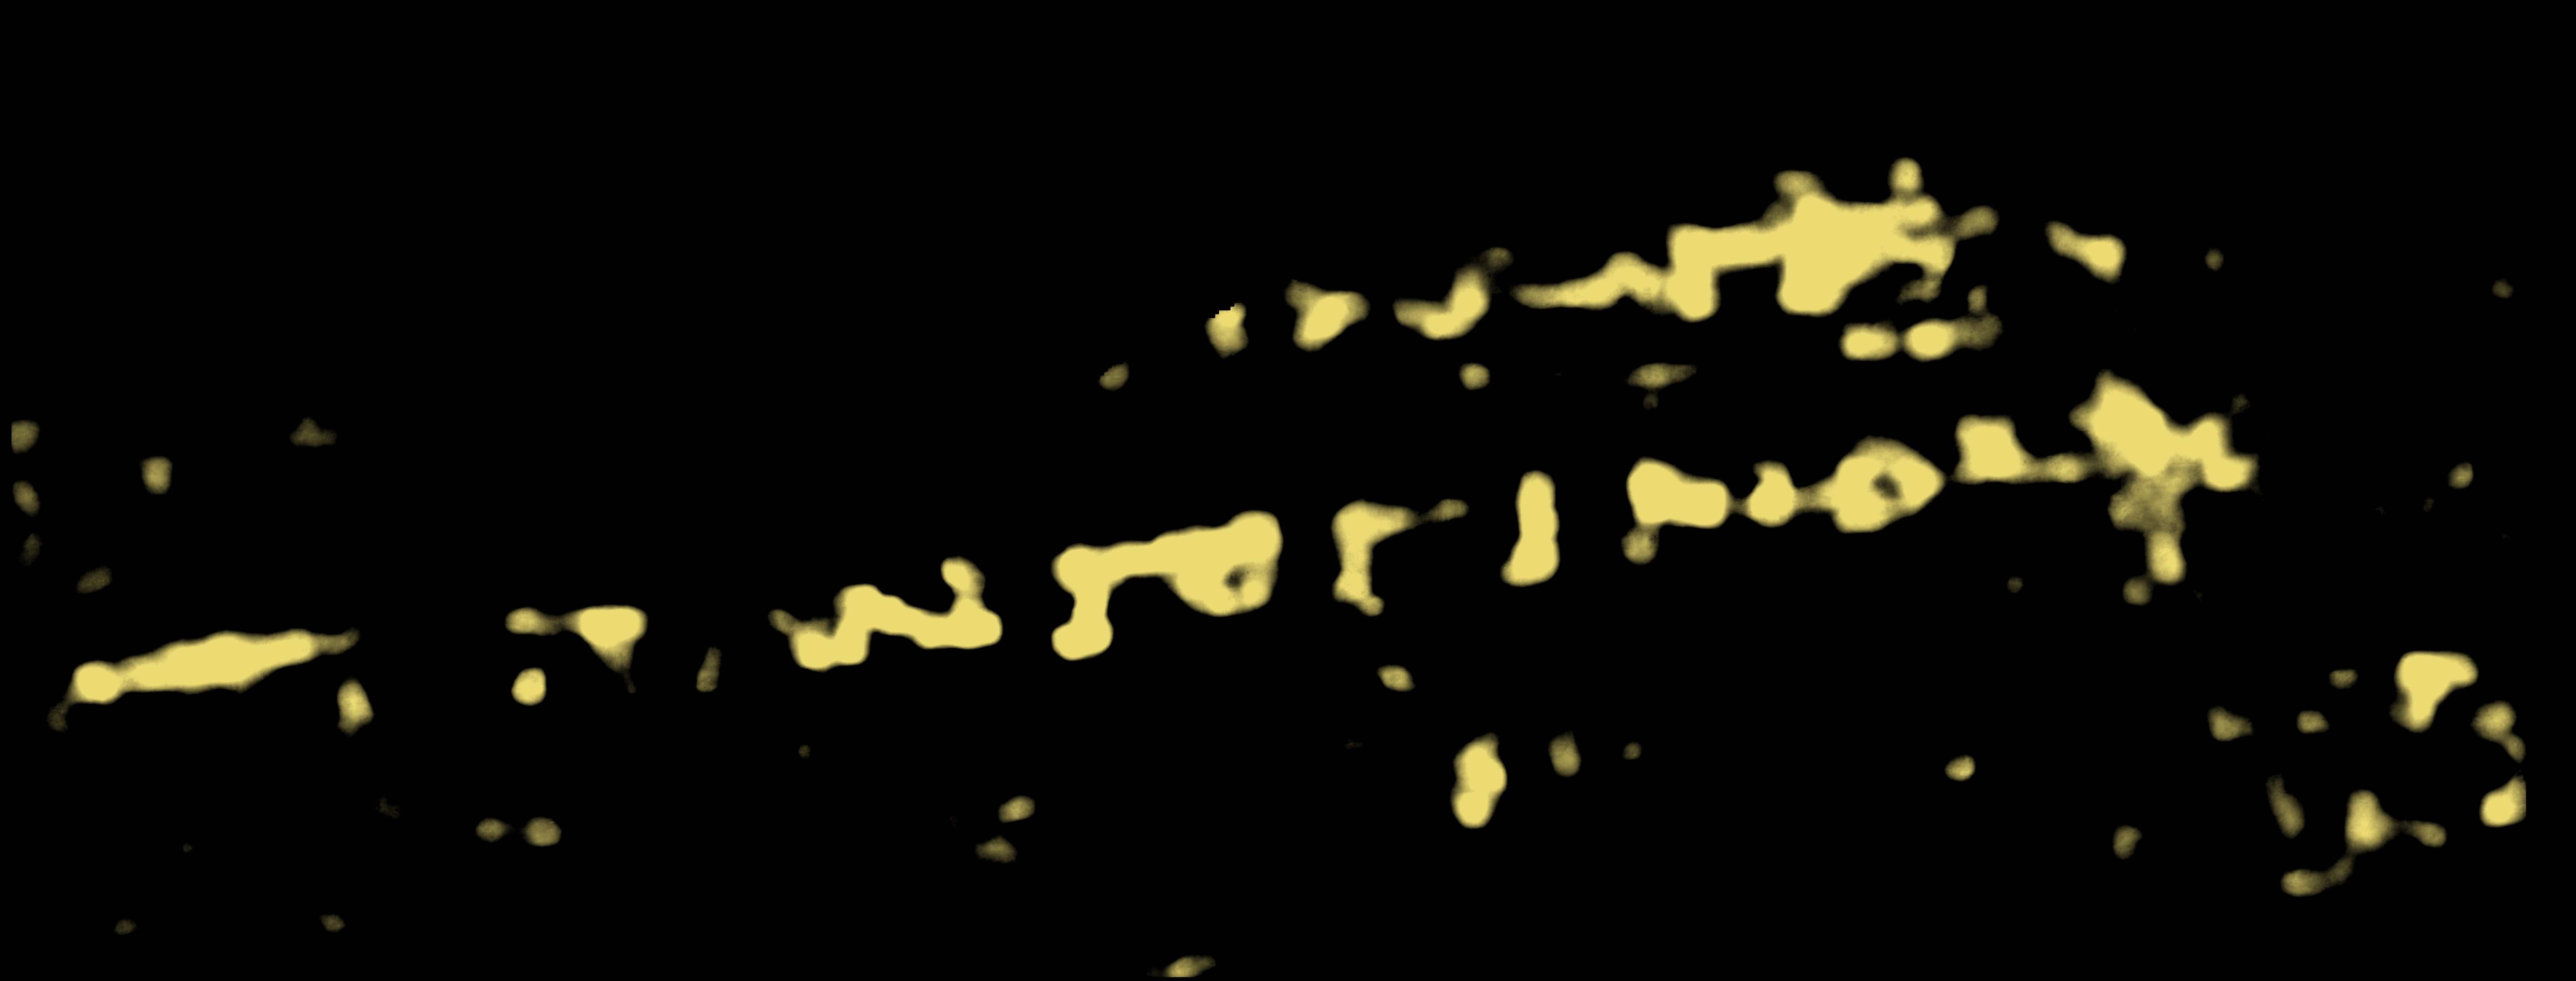
\includegraphics[width=122.48pt]{../figures/0343/0343_5_rectina-m1.png}}\end{minipage}}
\par\vspace{4pt}
\noindent\makebox[\columnwidth][c]{\begin{minipage}[t]{122.48pt}\centering\href{https://raw.githubusercontent.com/evilaliv3/vesuvius-challenge-pipeline/main/results/db27c806-rectina/src/figures/0343/0343_4_reader-v3.png}{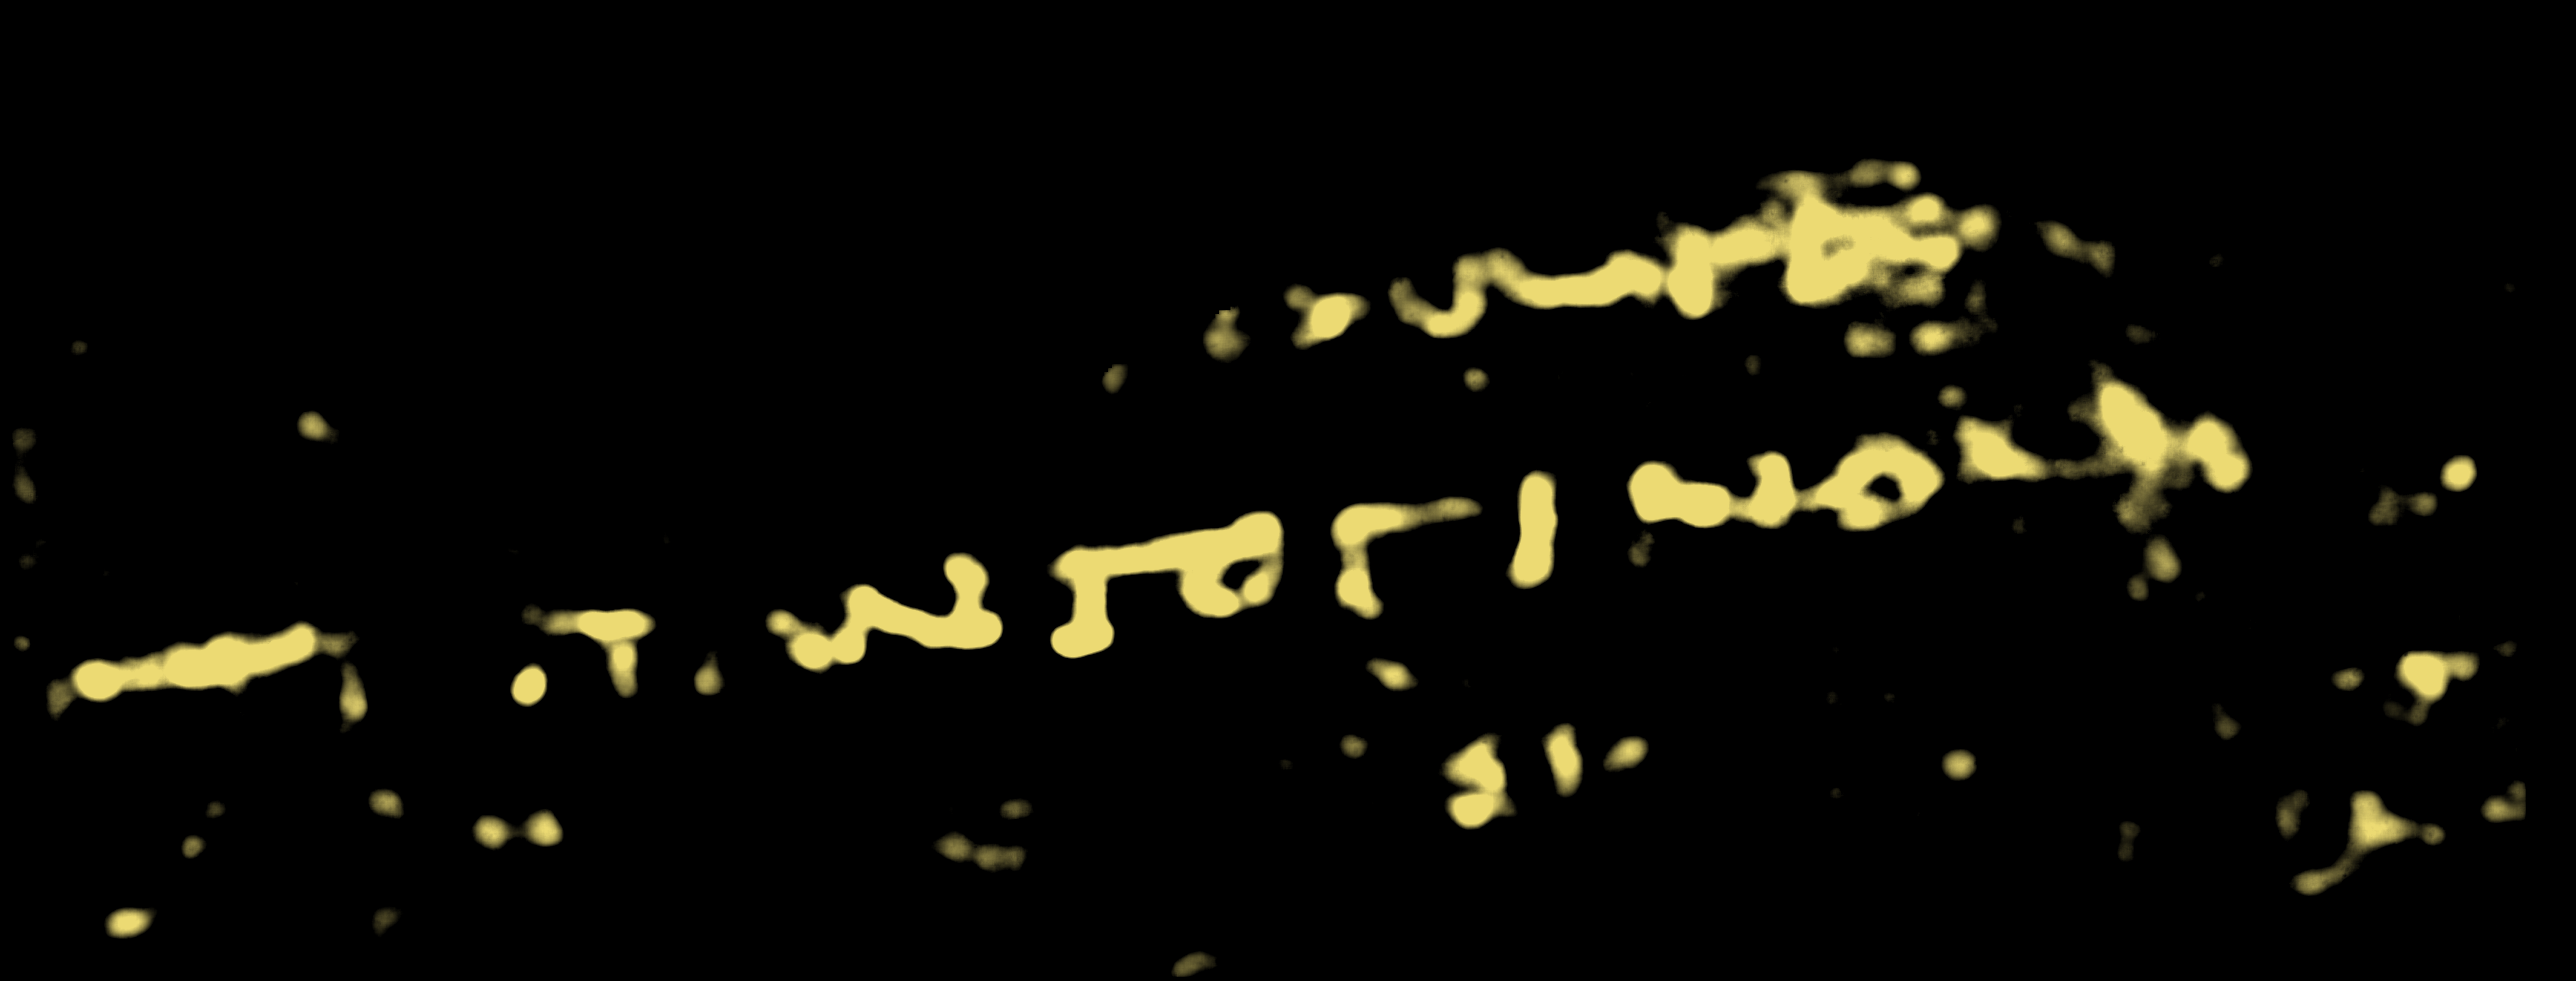
\includegraphics[width=122.48pt]{../figures/0343/0343_4_reader-v3.png}}\end{minipage}\hspace{2pt}\begin{minipage}[t]{122.48pt}\centering\href{https://raw.githubusercontent.com/evilaliv3/vesuvius-challenge-pipeline/main/results/db27c806-rectina/src/figures/0343/0343_6_rectina-m2.png}{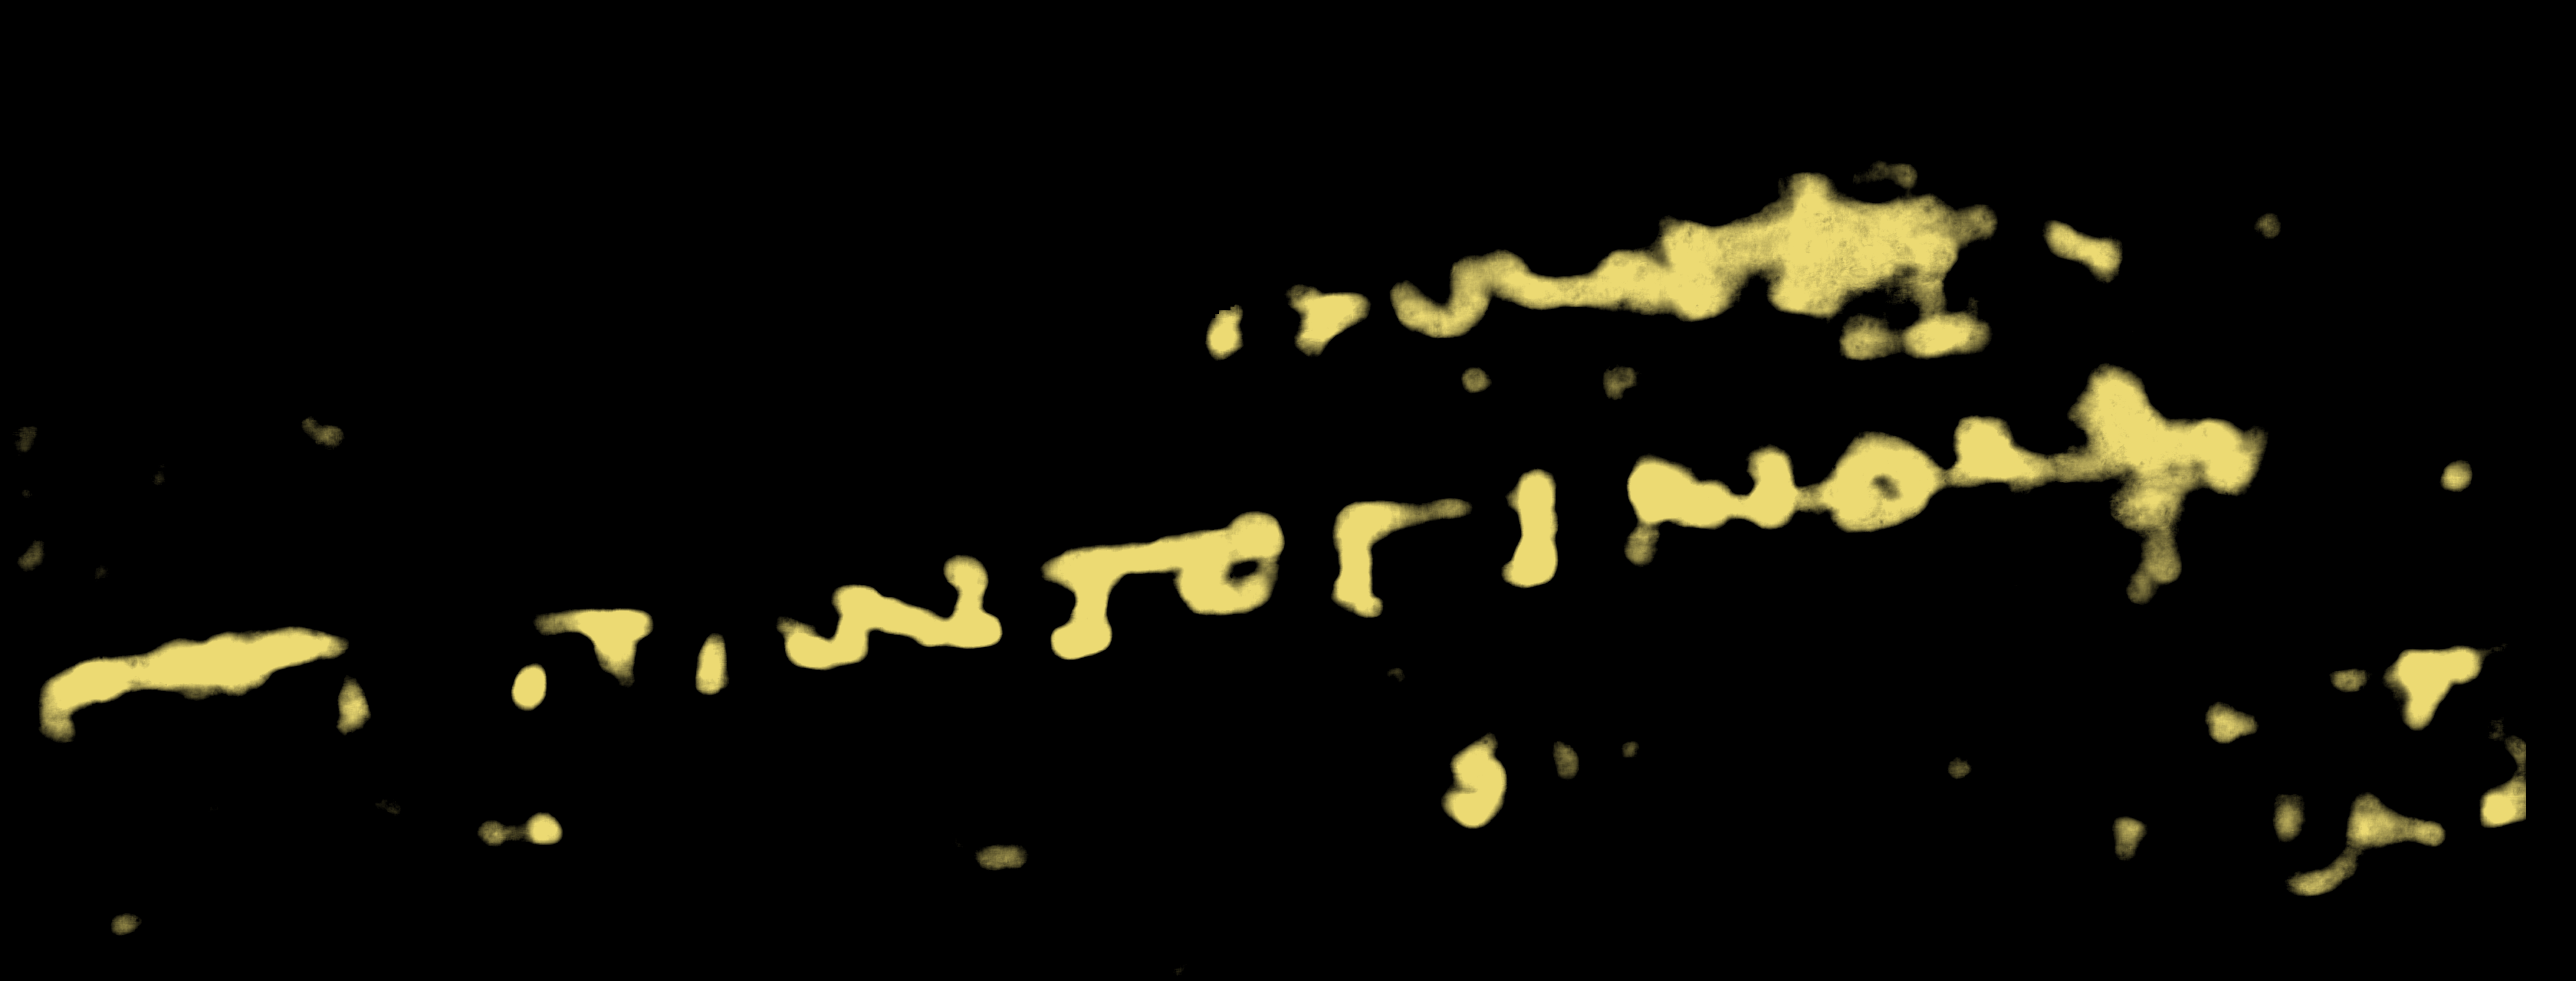
\includegraphics[width=122.48pt]{../figures/0343/0343_6_rectina-m2.png}}\end{minipage}}
\caption{Control unit 0343, three rows of two panels. Row 1: left, Texture; right, Labels. Row 2: left, Reader v2; right, Rectina m1 (display windows: Reader v2 0.409836 to 0.590749 (ramp); Rectina m1 0.548366 to 0.721975 (ramp)). Row 3: left, Reader v3; right, Rectina m2 (display windows: Reader v3 0.444697 to 0.678368 (ramp); Rectina m2 0.627931 to 0.765628 (ramp)). Each map is stretched between its own percentiles. The control is shown rotated 180 degrees, as the index of the panels records. Reader and model stand side by side in the rows 2 and 3.}
\end{figure}

\begin{figure}[!tbp]
\centering
\noindent\makebox[\columnwidth][c]{\begin{minipage}[t]{122.48pt}\centering\href{https://raw.githubusercontent.com/evilaliv3/vesuvius-challenge-pipeline/main/results/db27c806-rectina/src/figures/w058/w058_1_texture.png}{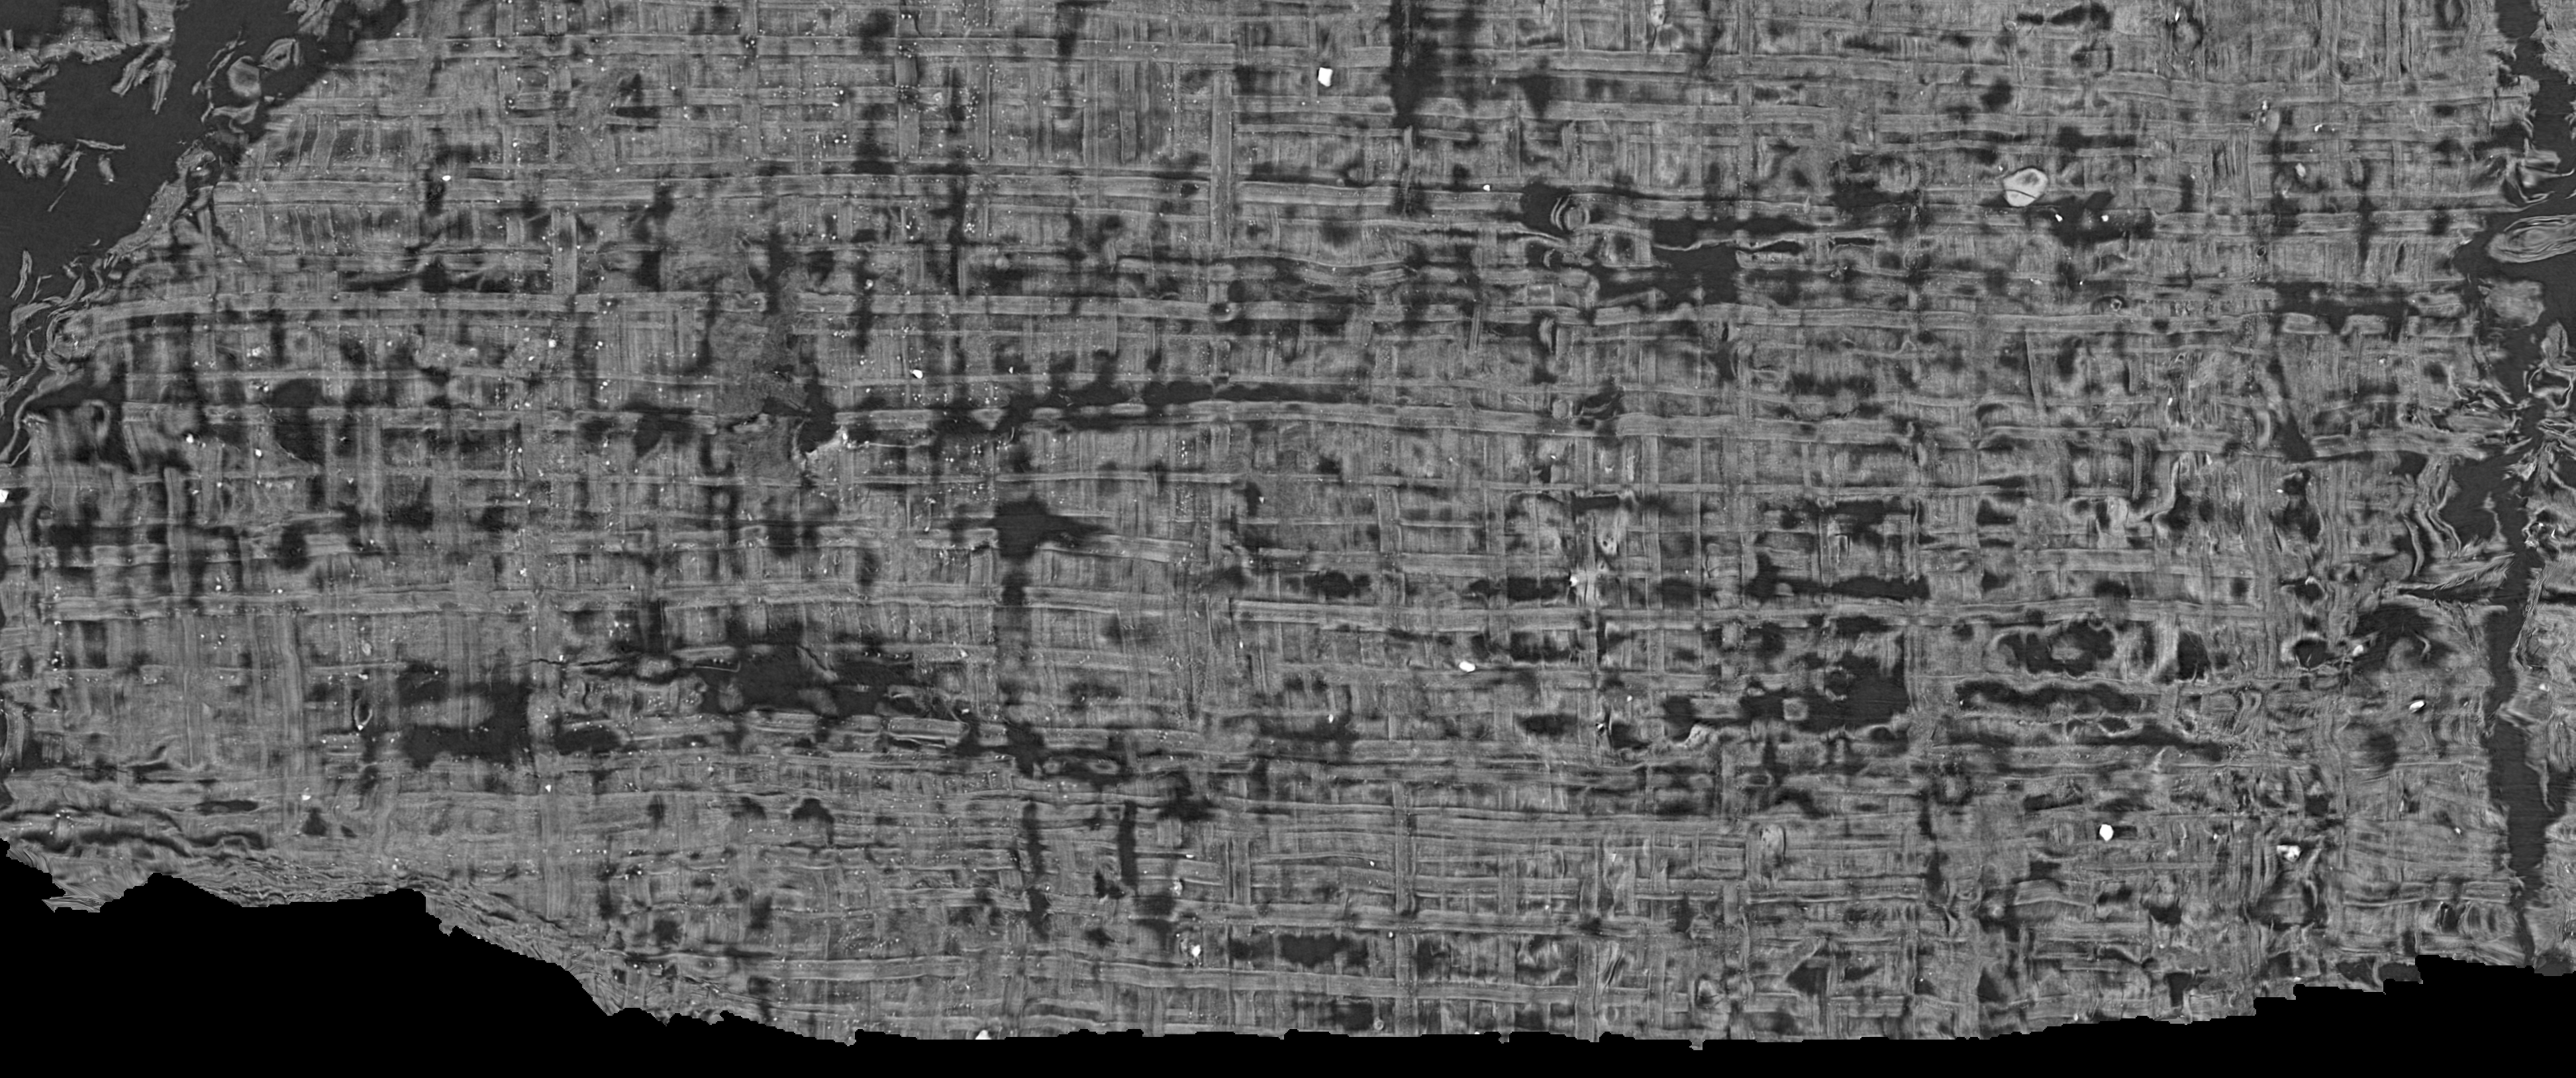
\includegraphics[width=122.48pt]{../figures/w058/w058_1_texture.png}}\end{minipage}\hspace{2pt}\begin{minipage}[t]{122.48pt}\centering\href{https://raw.githubusercontent.com/evilaliv3/vesuvius-challenge-pipeline/main/results/db27c806-rectina/src/figures/w058/w058_2_labels.png}{
\includegraphics[width=122.48pt]{../figures/w058/w058_2_labels.png}}\end{minipage}}
\par\vspace{4pt}
\noindent\makebox[\columnwidth][c]{\begin{minipage}[t]{122.48pt}\centering\href{https://raw.githubusercontent.com/evilaliv3/vesuvius-challenge-pipeline/main/results/db27c806-rectina/src/figures/w058/w058_3_reader-v2.png}{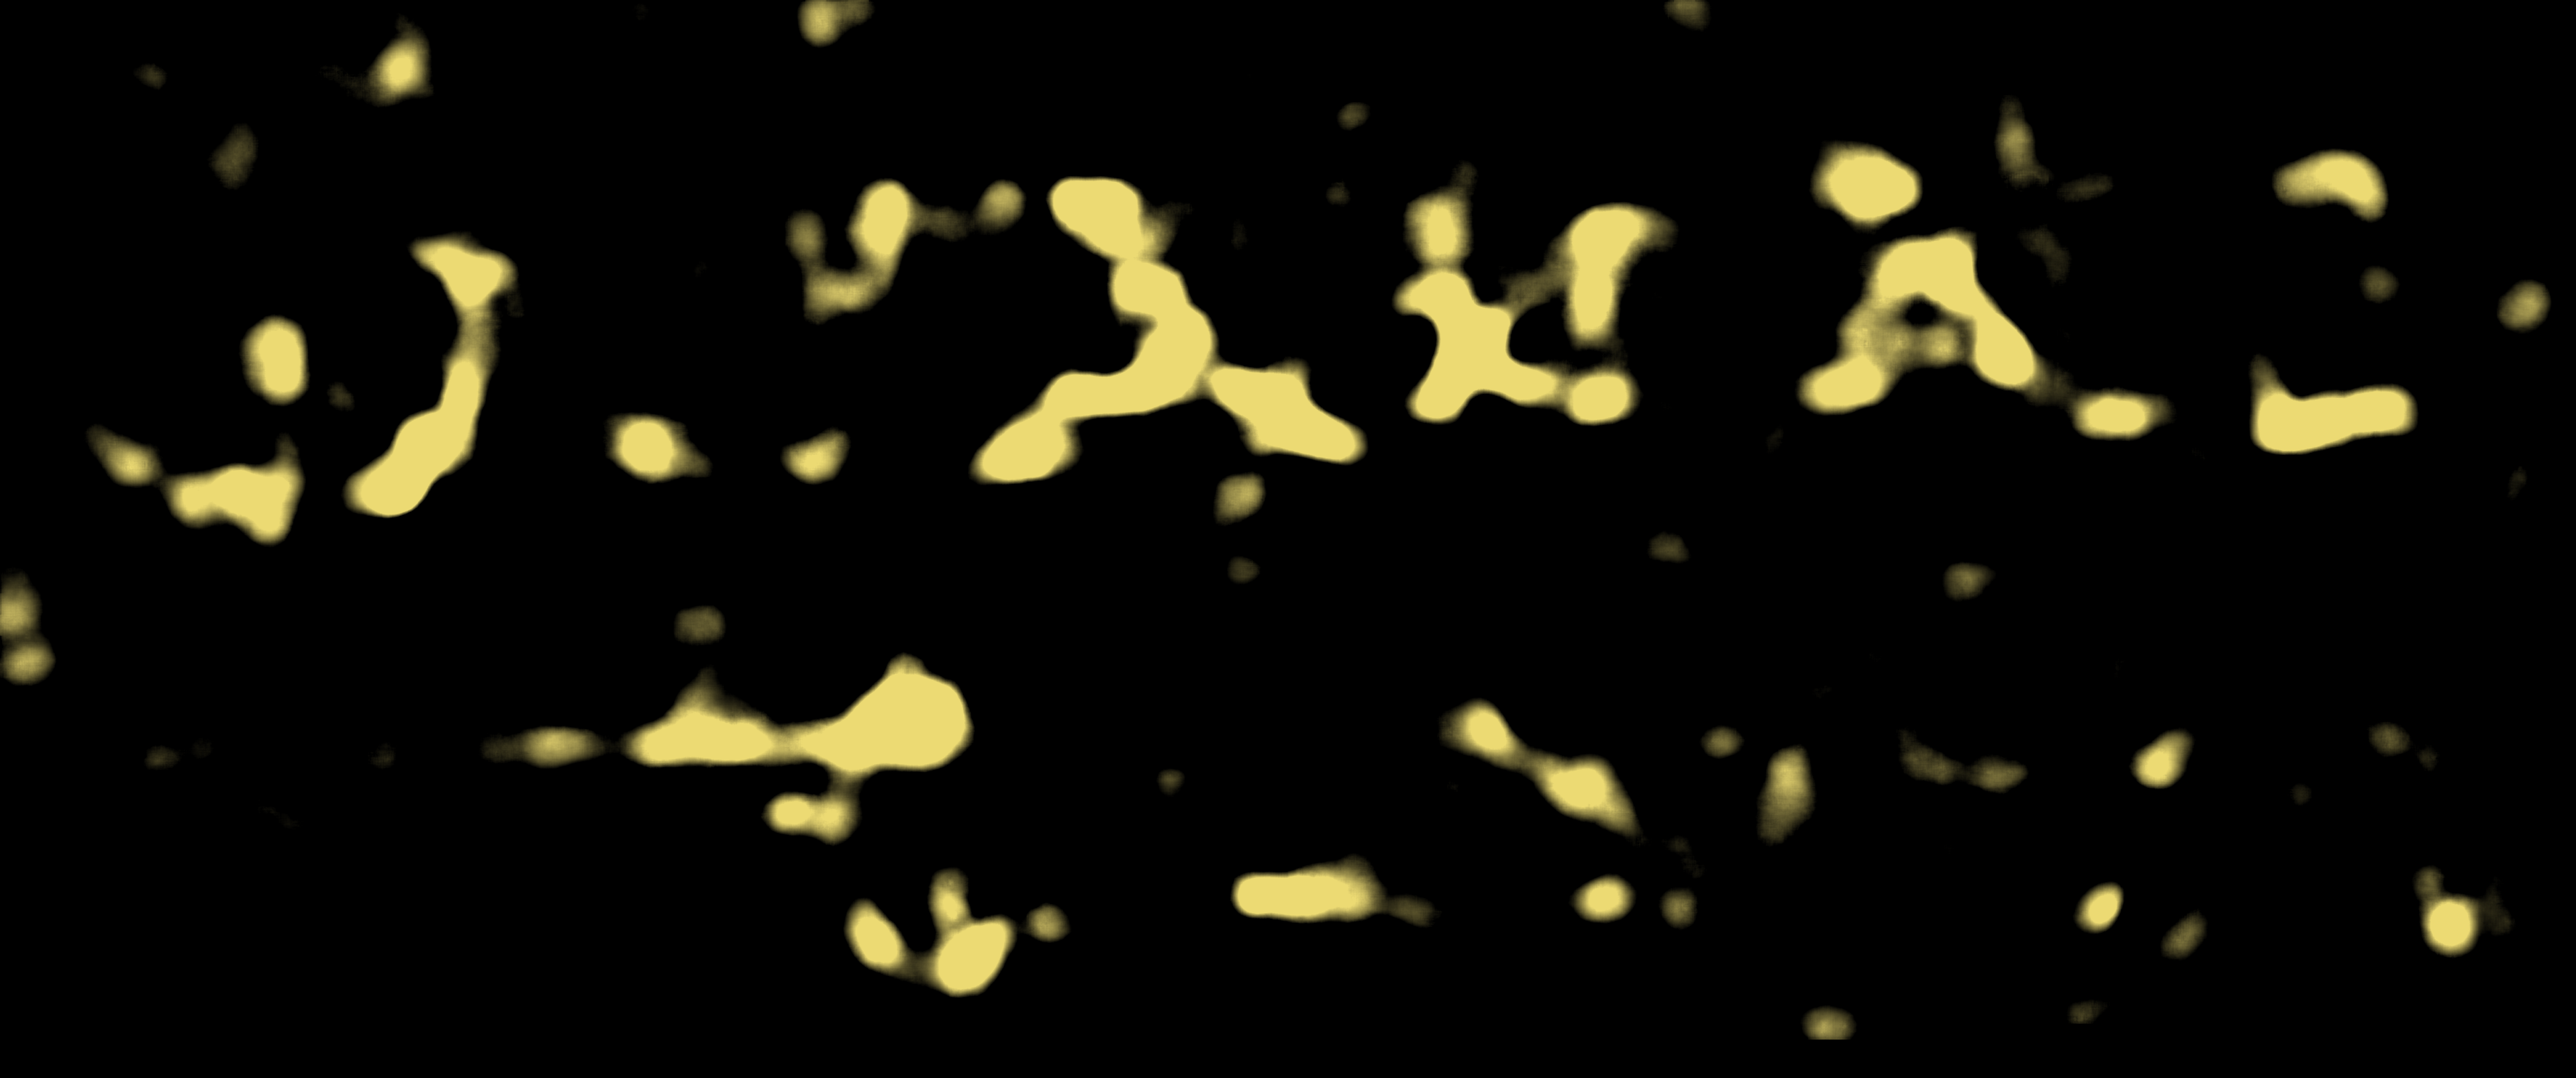
\includegraphics[width=122.48pt]{../figures/w058/w058_3_reader-v2.png}}\end{minipage}\hspace{2pt}\begin{minipage}[t]{122.48pt}\centering\href{https://raw.githubusercontent.com/evilaliv3/vesuvius-challenge-pipeline/main/results/db27c806-rectina/src/figures/w058/w058_5_rectina-m1.png}{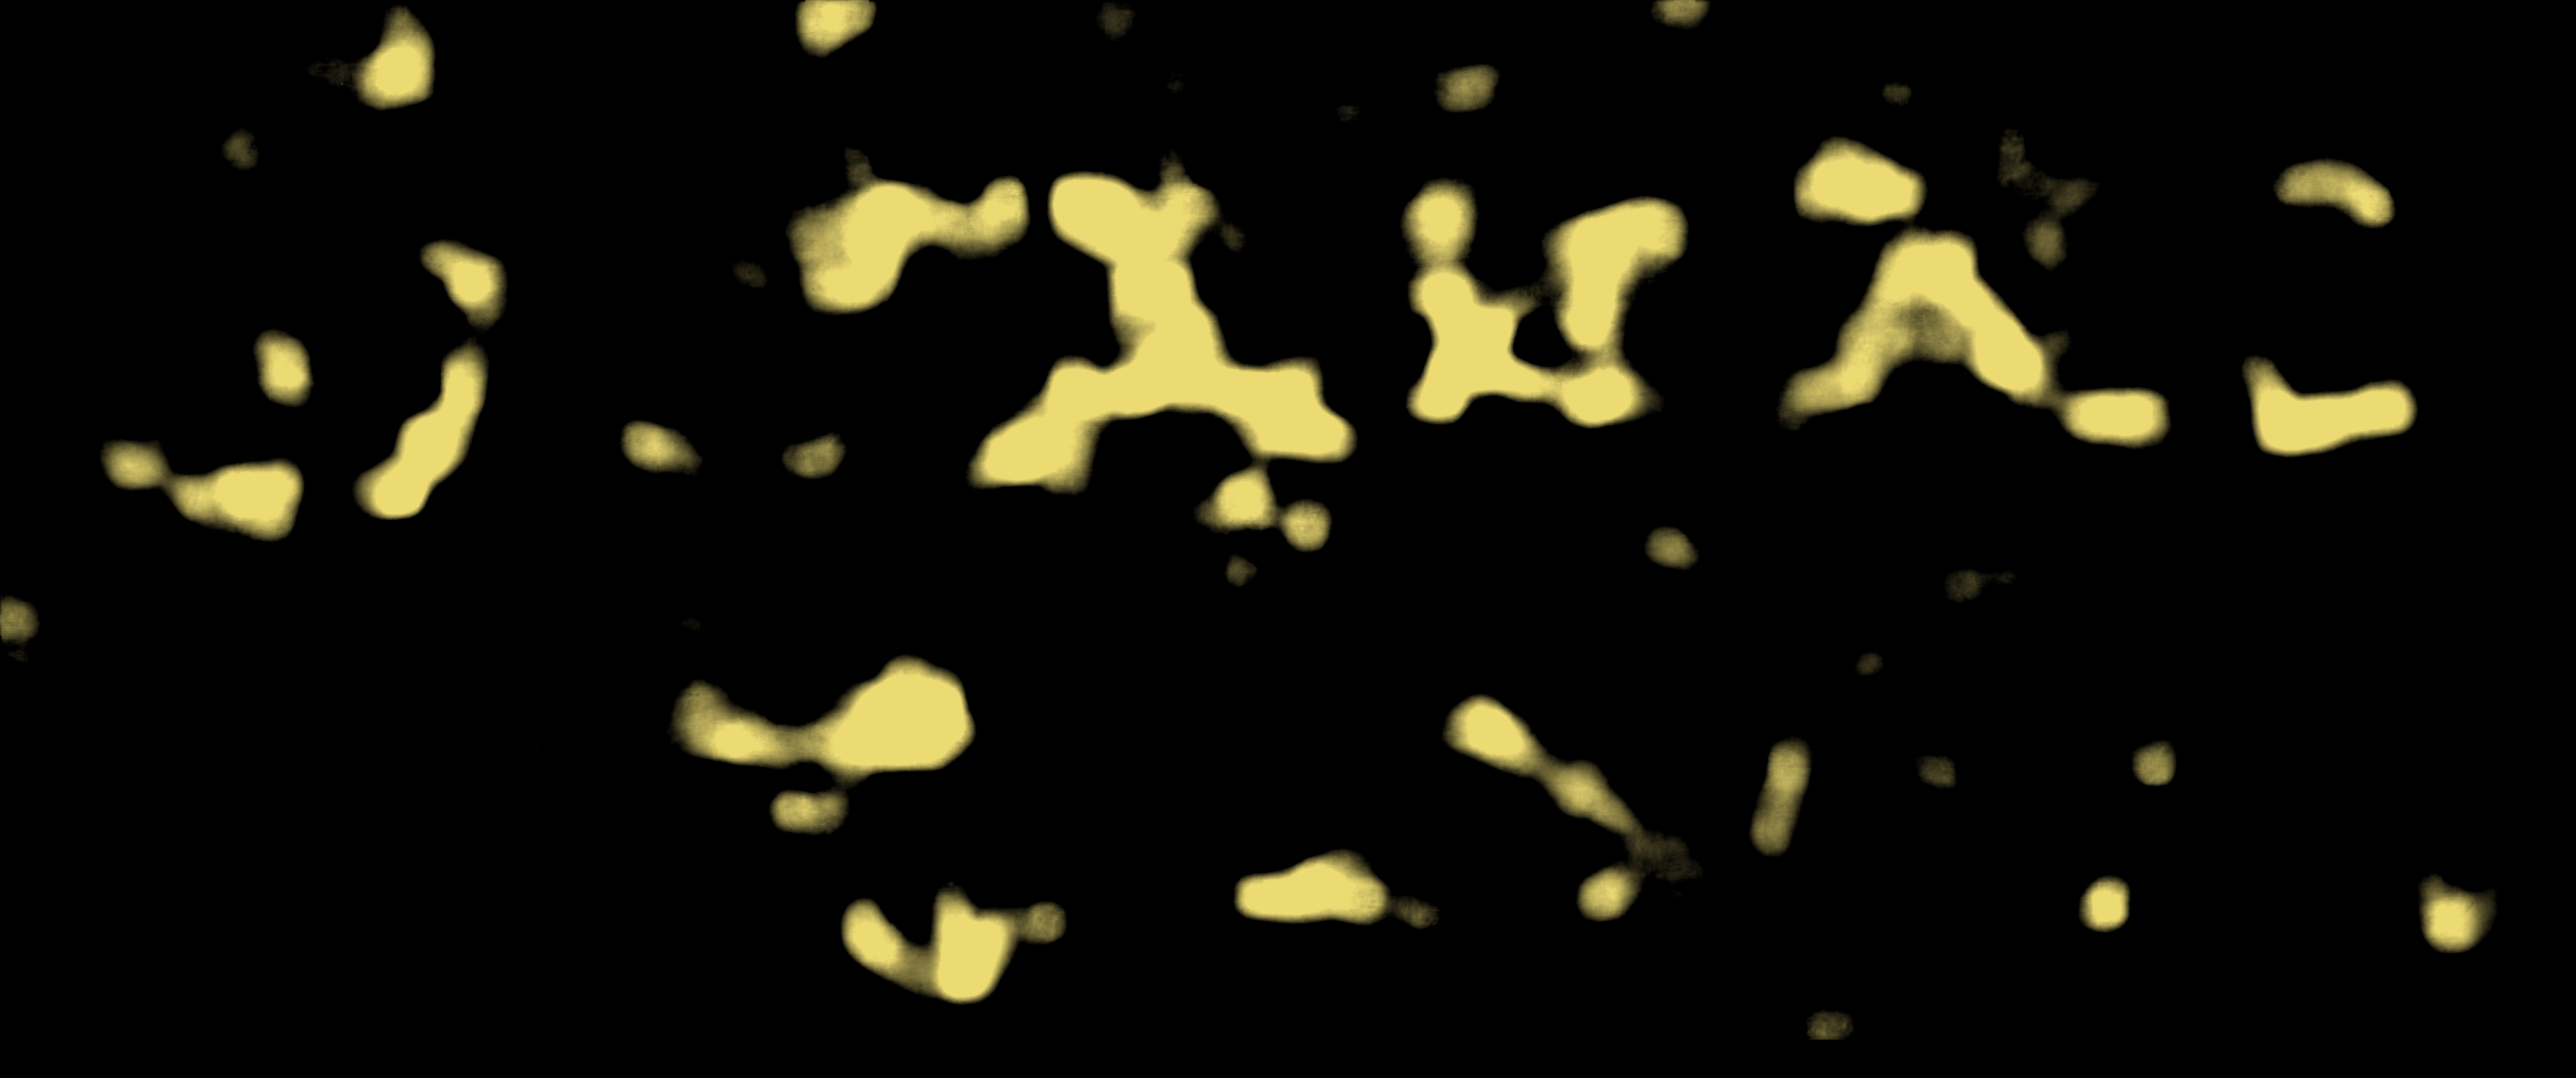
\includegraphics[width=122.48pt]{../figures/w058/w058_5_rectina-m1.png}}\end{minipage}}
\par\vspace{4pt}
\noindent\makebox[\columnwidth][c]{\begin{minipage}[t]{122.48pt}\centering\href{https://raw.githubusercontent.com/evilaliv3/vesuvius-challenge-pipeline/main/results/db27c806-rectina/src/figures/w058/w058_4_reader-v3.png}{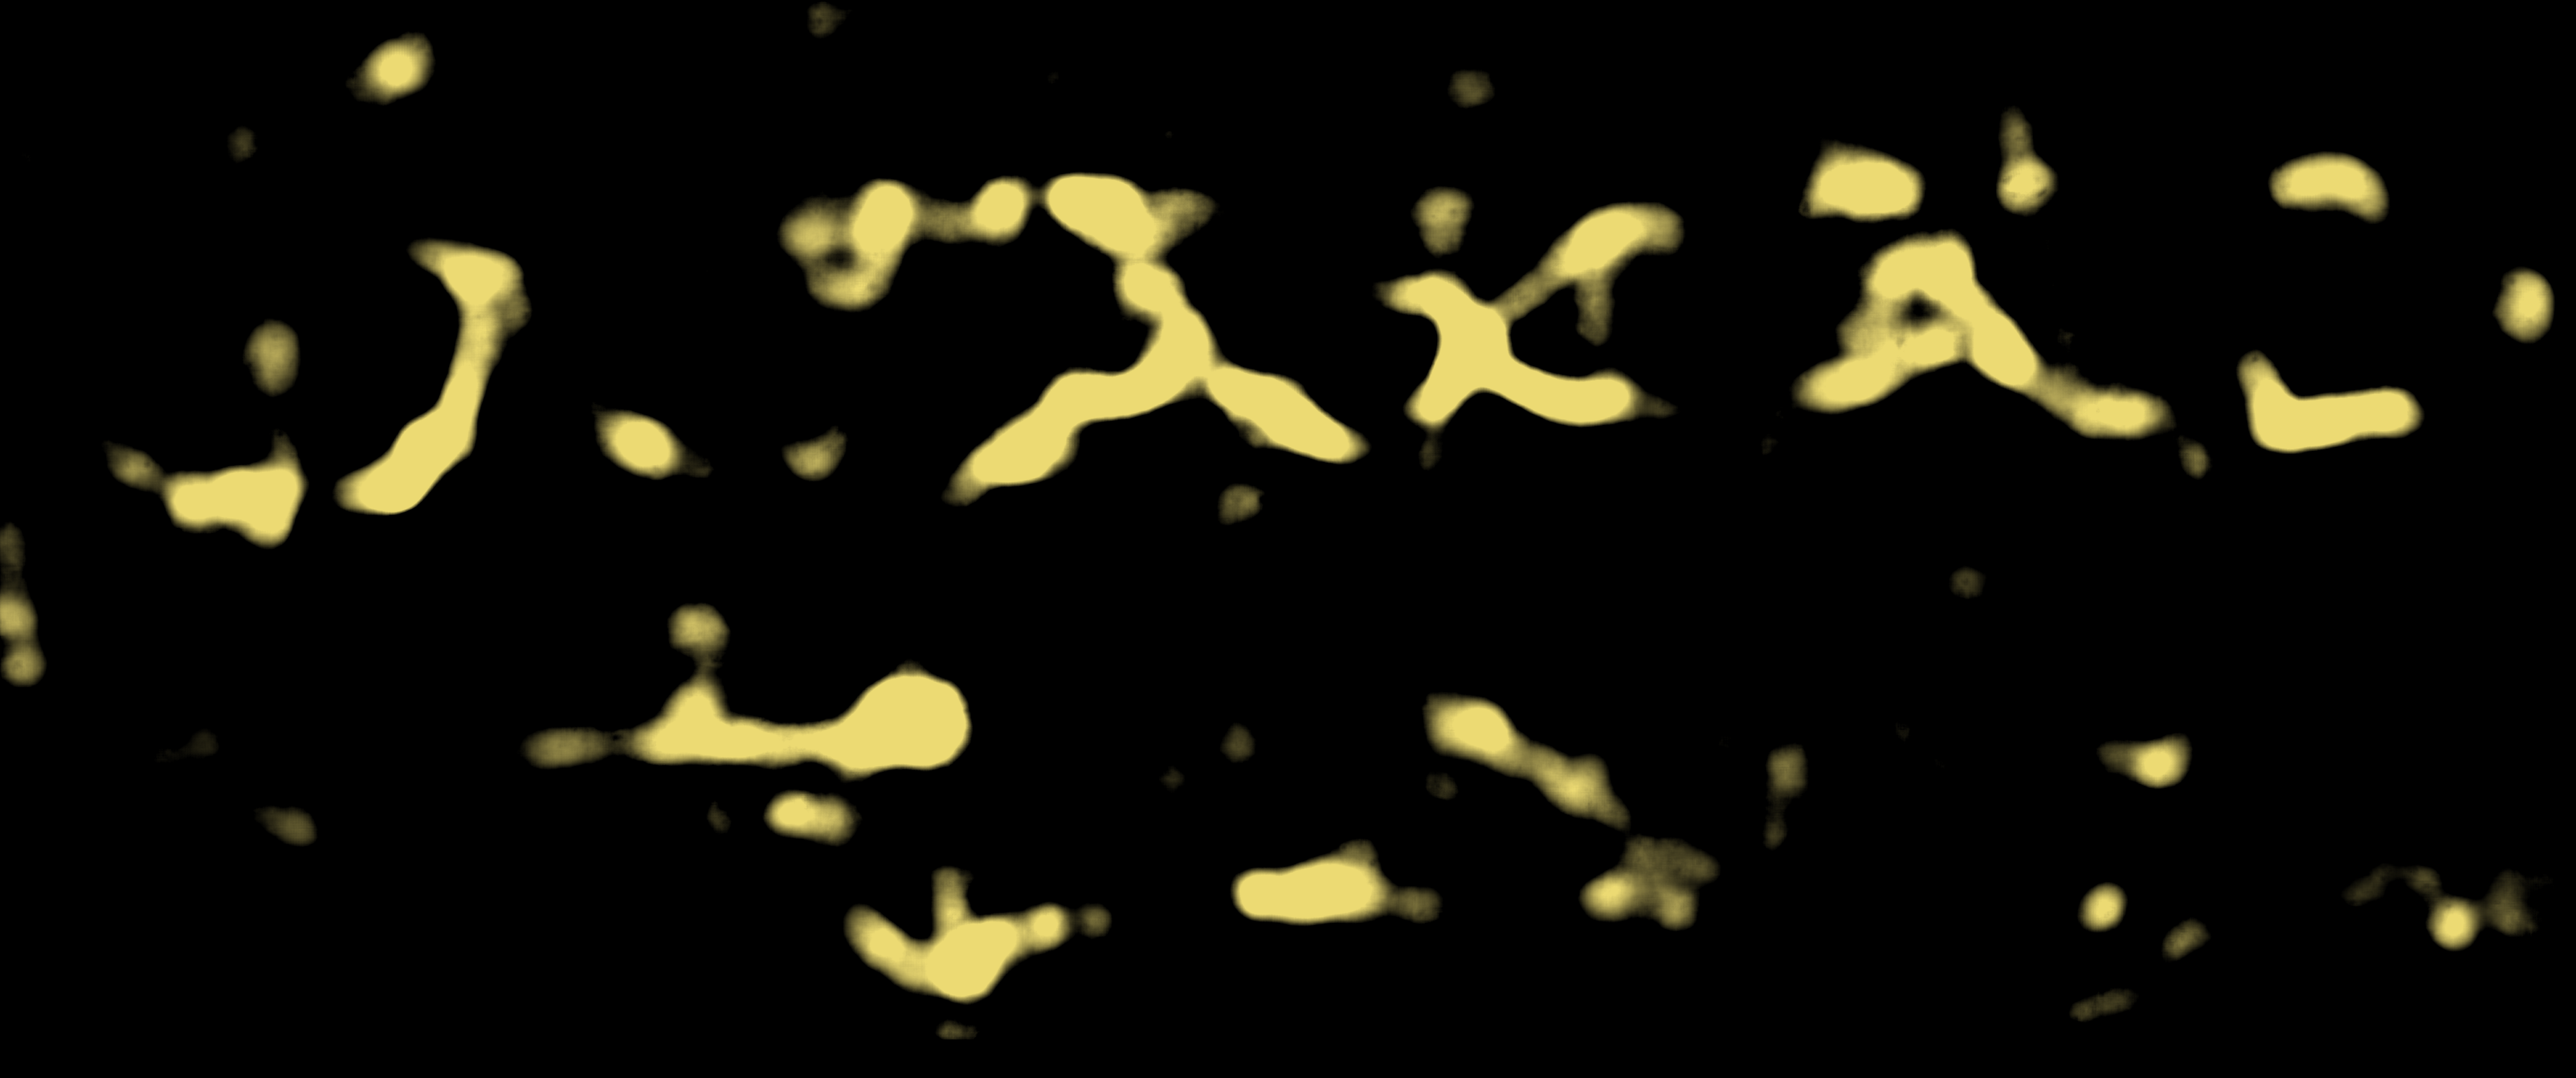
\includegraphics[width=122.48pt]{../figures/w058/w058_4_reader-v3.png}}\end{minipage}\hspace{2pt}\begin{minipage}[t]{122.48pt}\centering\href{https://raw.githubusercontent.com/evilaliv3/vesuvius-challenge-pipeline/main/results/db27c806-rectina/src/figures/w058/w058_6_rectina-m2.png}{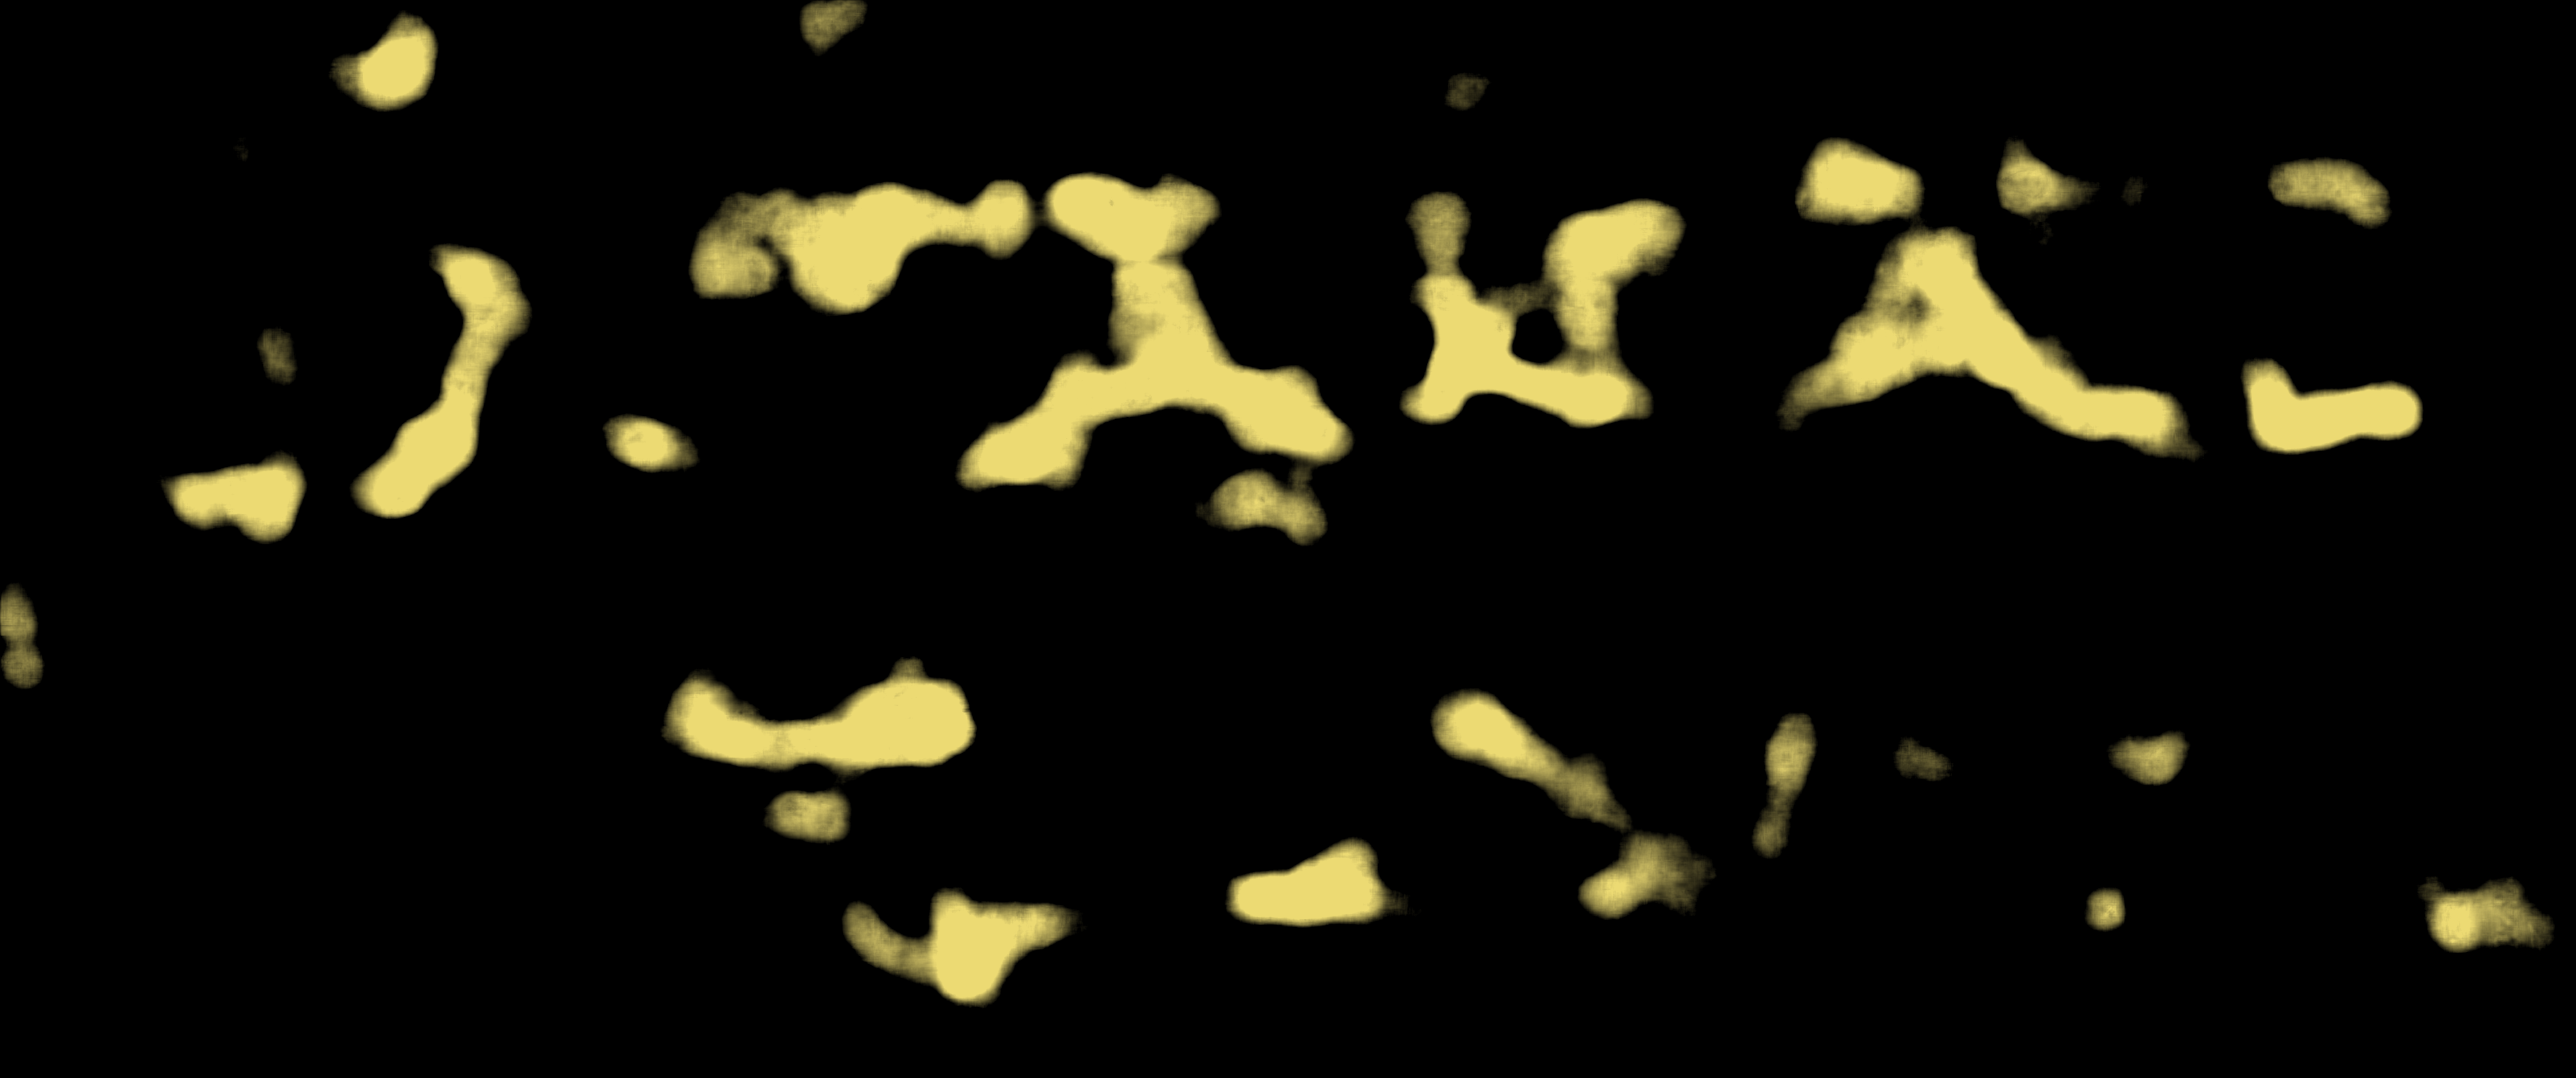
\includegraphics[width=122.48pt]{../figures/w058/w058_6_rectina-m2.png}}\end{minipage}}
\caption{Control unit 1447 w058, three rows of two panels. Row 1: left, Texture; right, Labels. Row 2: left, Reader v2; right, Rectina m1 (display windows: Reader v2 0.385394 to 0.561662 (ramp); Rectina m1 0.533701 to 0.711716 (ramp)). Row 3: left, Reader v3; right, Rectina m2 (display windows: Reader v3 0.450583 to 0.670398 (ramp); Rectina m2 0.625307 to 0.773366 (ramp)). Each map is stretched between its own percentiles. Reader and model stand side by side in the rows 2 and 3.}
\end{figure}

\begin{figure}[!tbp]
\centering
\noindent\makebox[\columnwidth][c]{\begin{minipage}[t]{122.48pt}\centering\href{https://raw.githubusercontent.com/evilaliv3/vesuvius-challenge-pipeline/main/results/db27c806-rectina/src/figures/w060/w060_1_texture.png}{
\includegraphics[width=122.48pt]{../figures/w060/w060_1_texture.png}}\end{minipage}\hspace{2pt}\begin{minipage}[t]{122.48pt}\centering\href{https://raw.githubusercontent.com/evilaliv3/vesuvius-challenge-pipeline/main/results/db27c806-rectina/src/figures/w060/w060_2_labels.png}{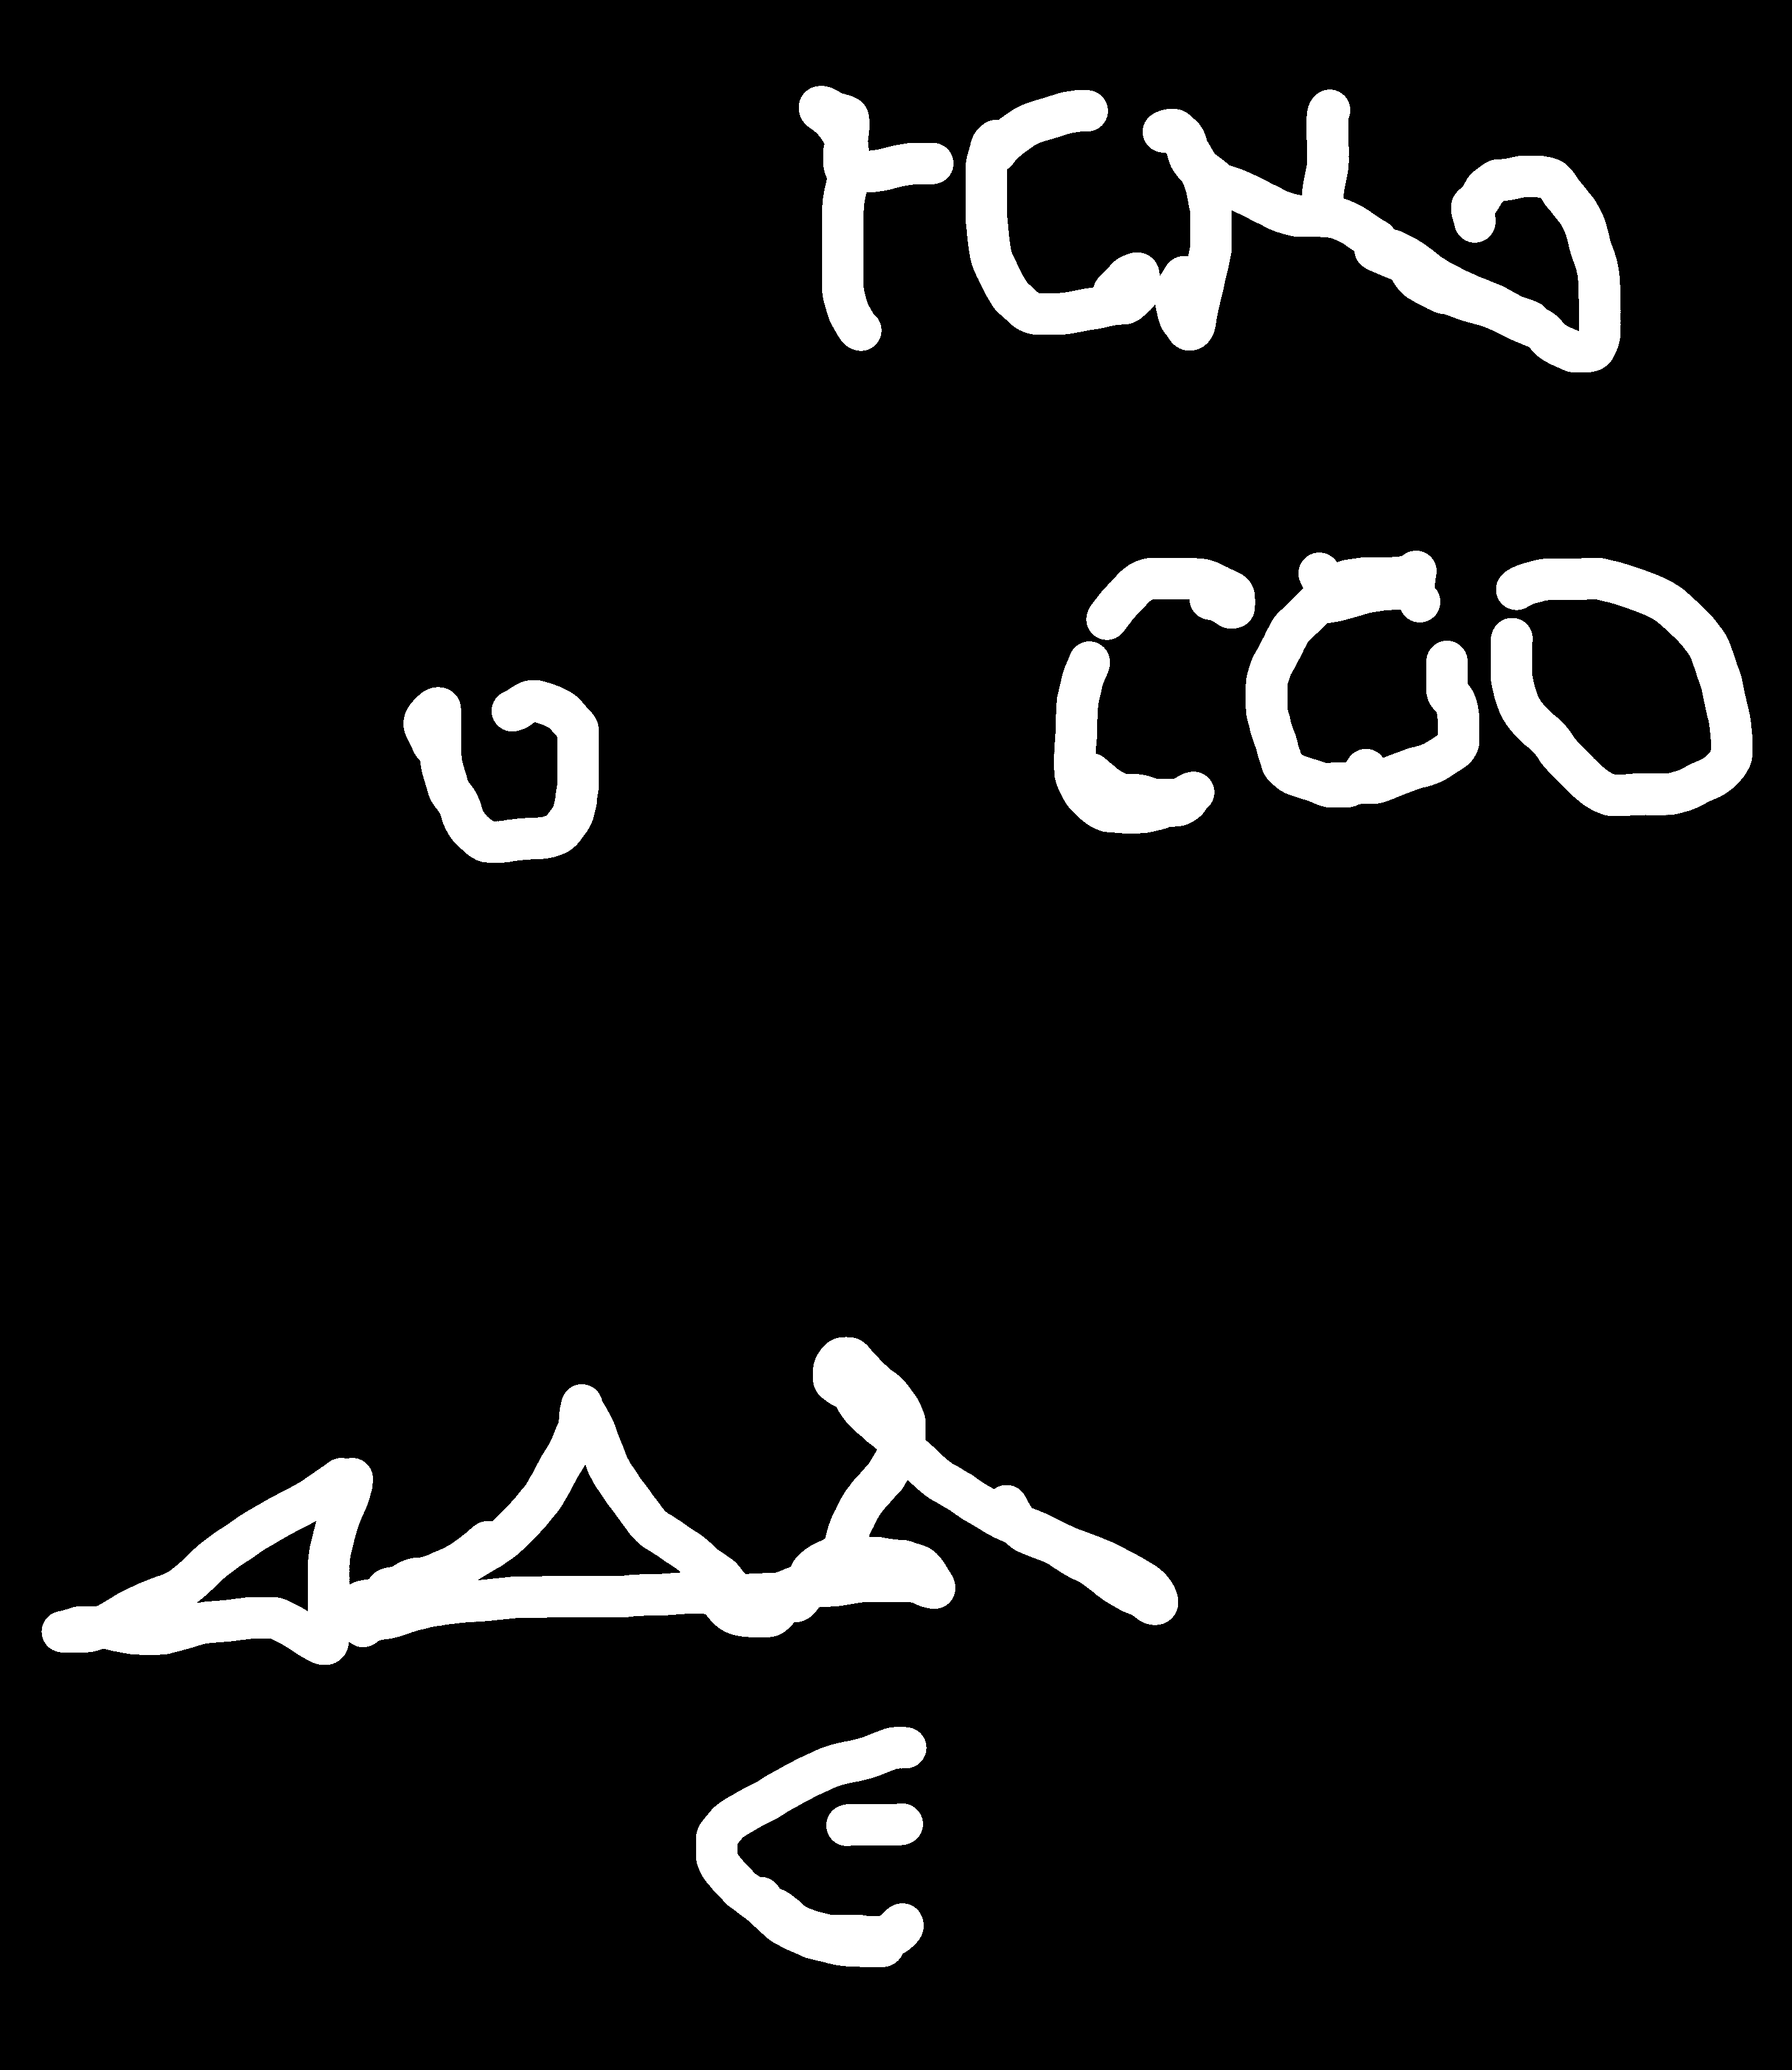
\includegraphics[width=122.48pt]{../figures/w060/w060_2_labels.png}}\end{minipage}}
\par\vspace{4pt}
\noindent\makebox[\columnwidth][c]{\begin{minipage}[t]{122.48pt}\centering\href{https://raw.githubusercontent.com/evilaliv3/vesuvius-challenge-pipeline/main/results/db27c806-rectina/src/figures/w060/w060_3_reader-v2.png}{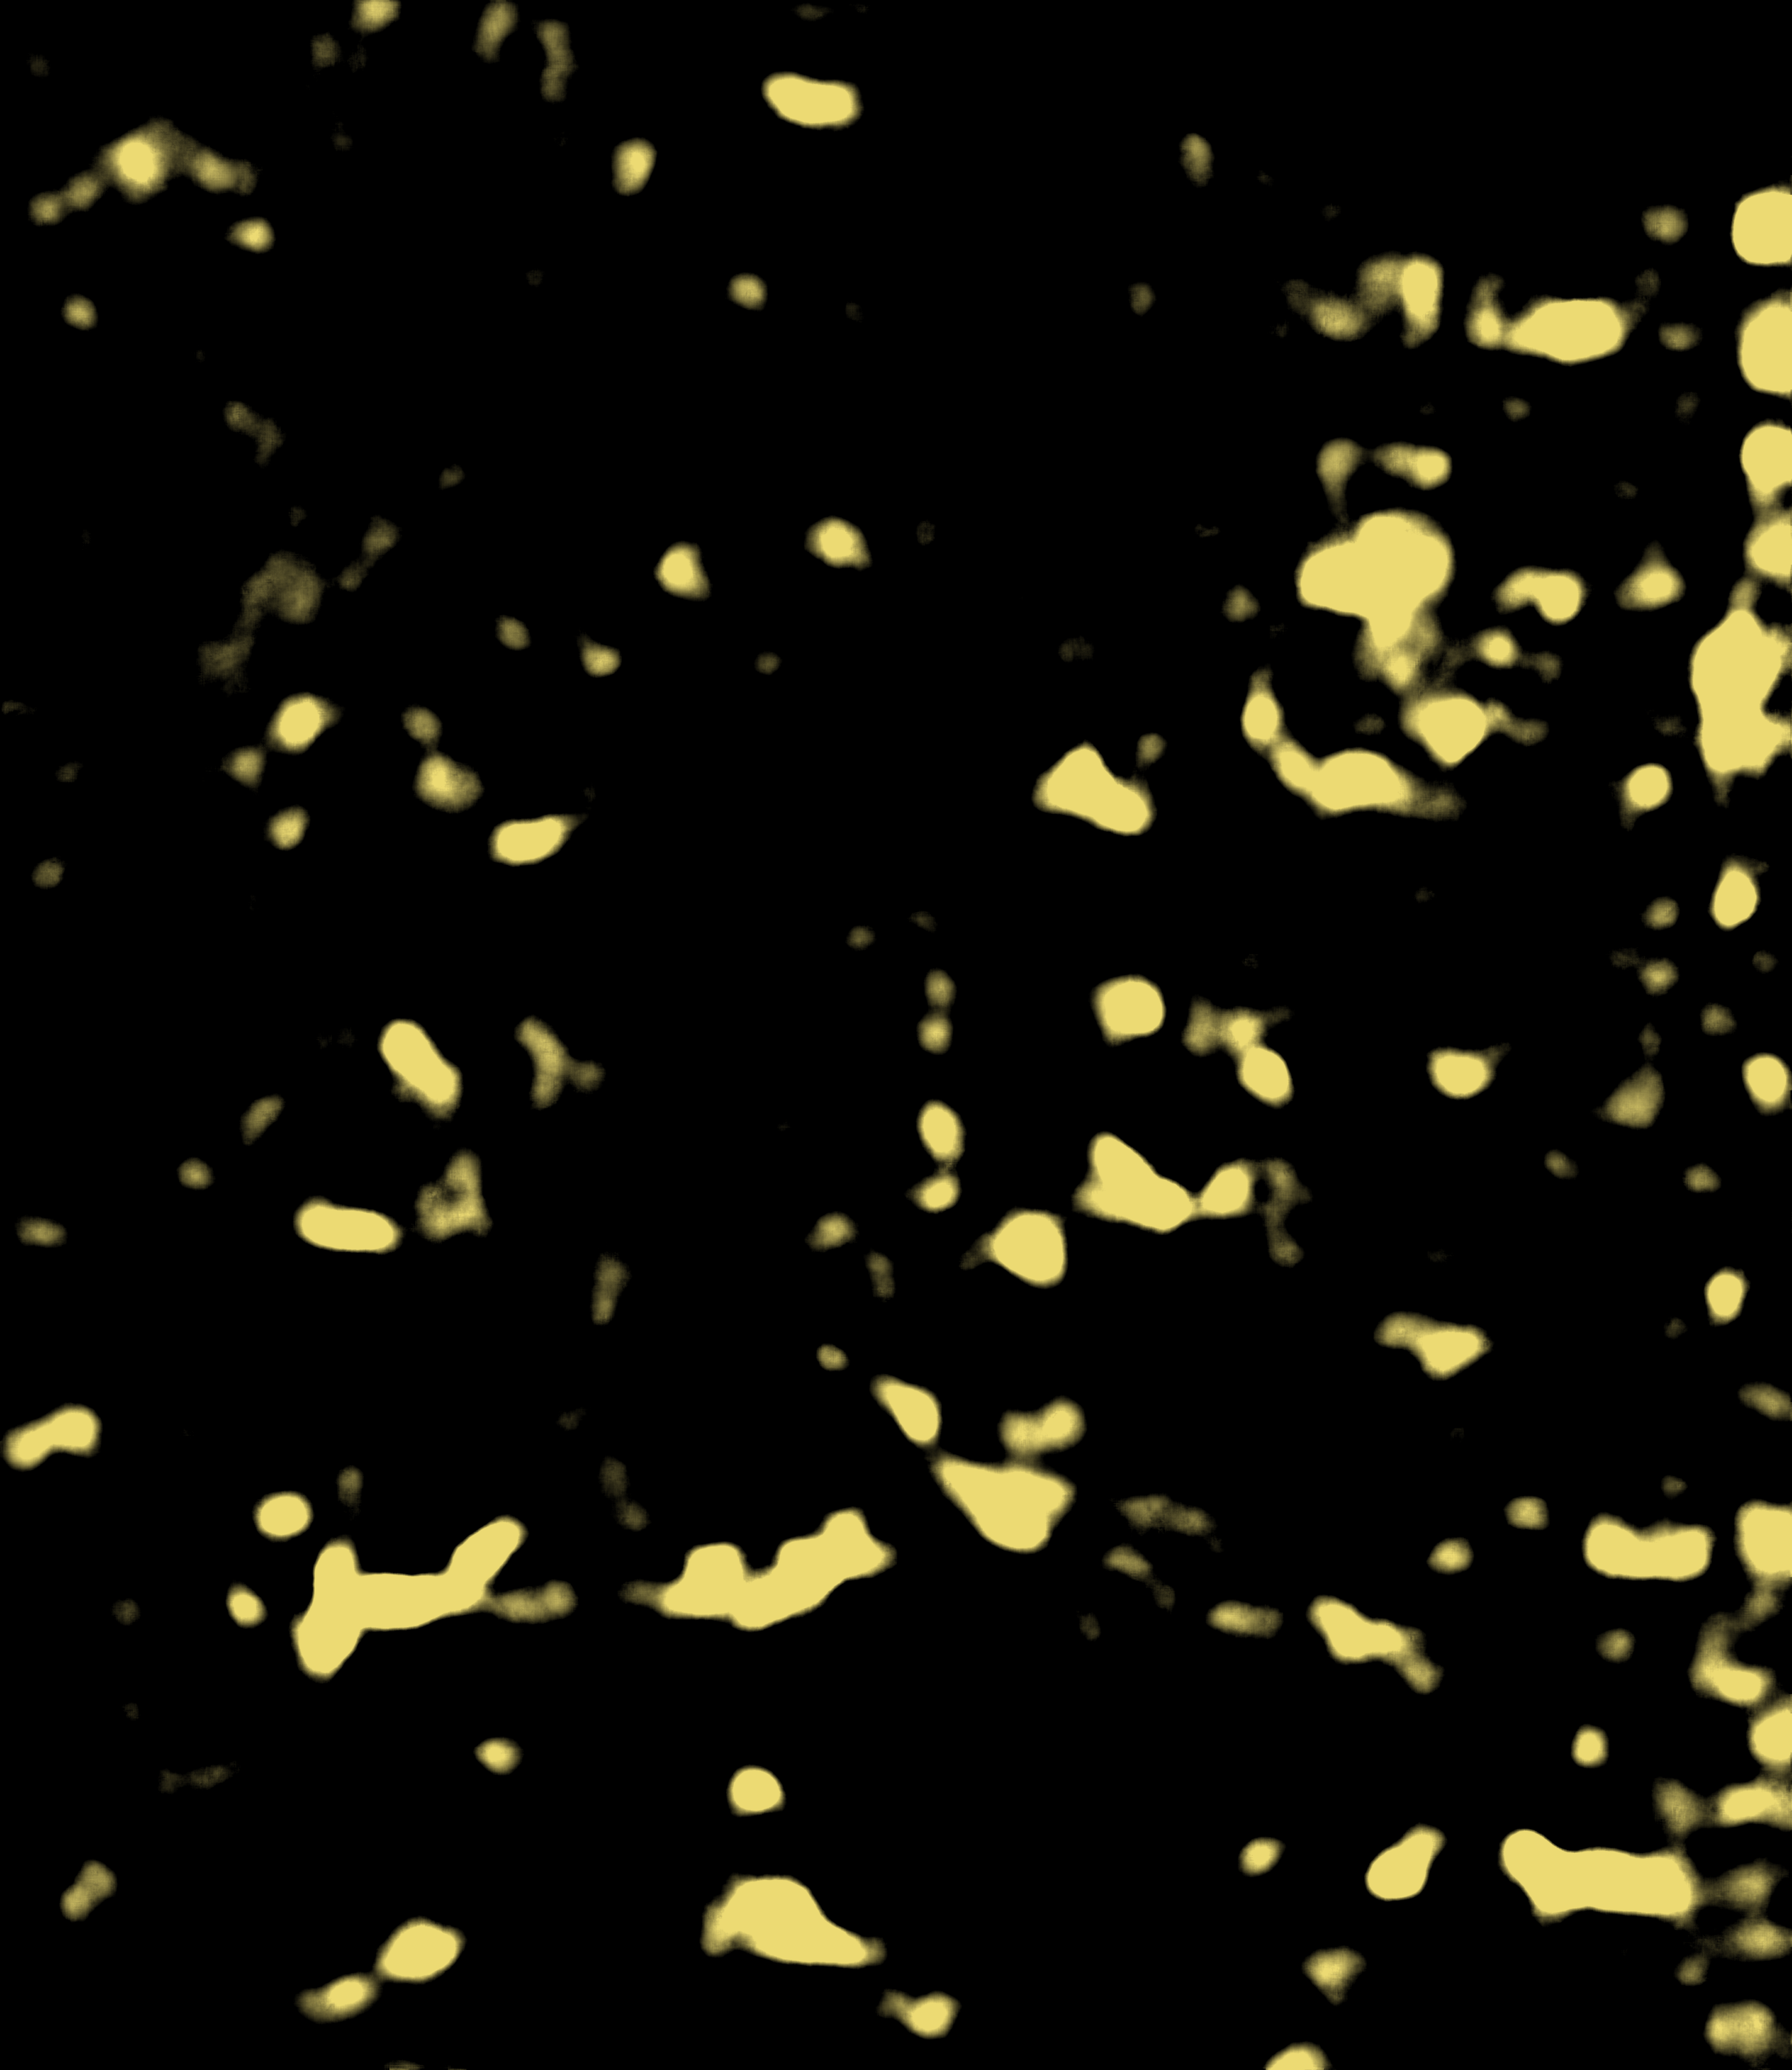
\includegraphics[width=122.48pt]{../figures/w060/w060_3_reader-v2.png}}\end{minipage}\hspace{2pt}\begin{minipage}[t]{122.48pt}\centering\href{https://raw.githubusercontent.com/evilaliv3/vesuvius-challenge-pipeline/main/results/db27c806-rectina/src/figures/w060/w060_5_rectina-m1.png}{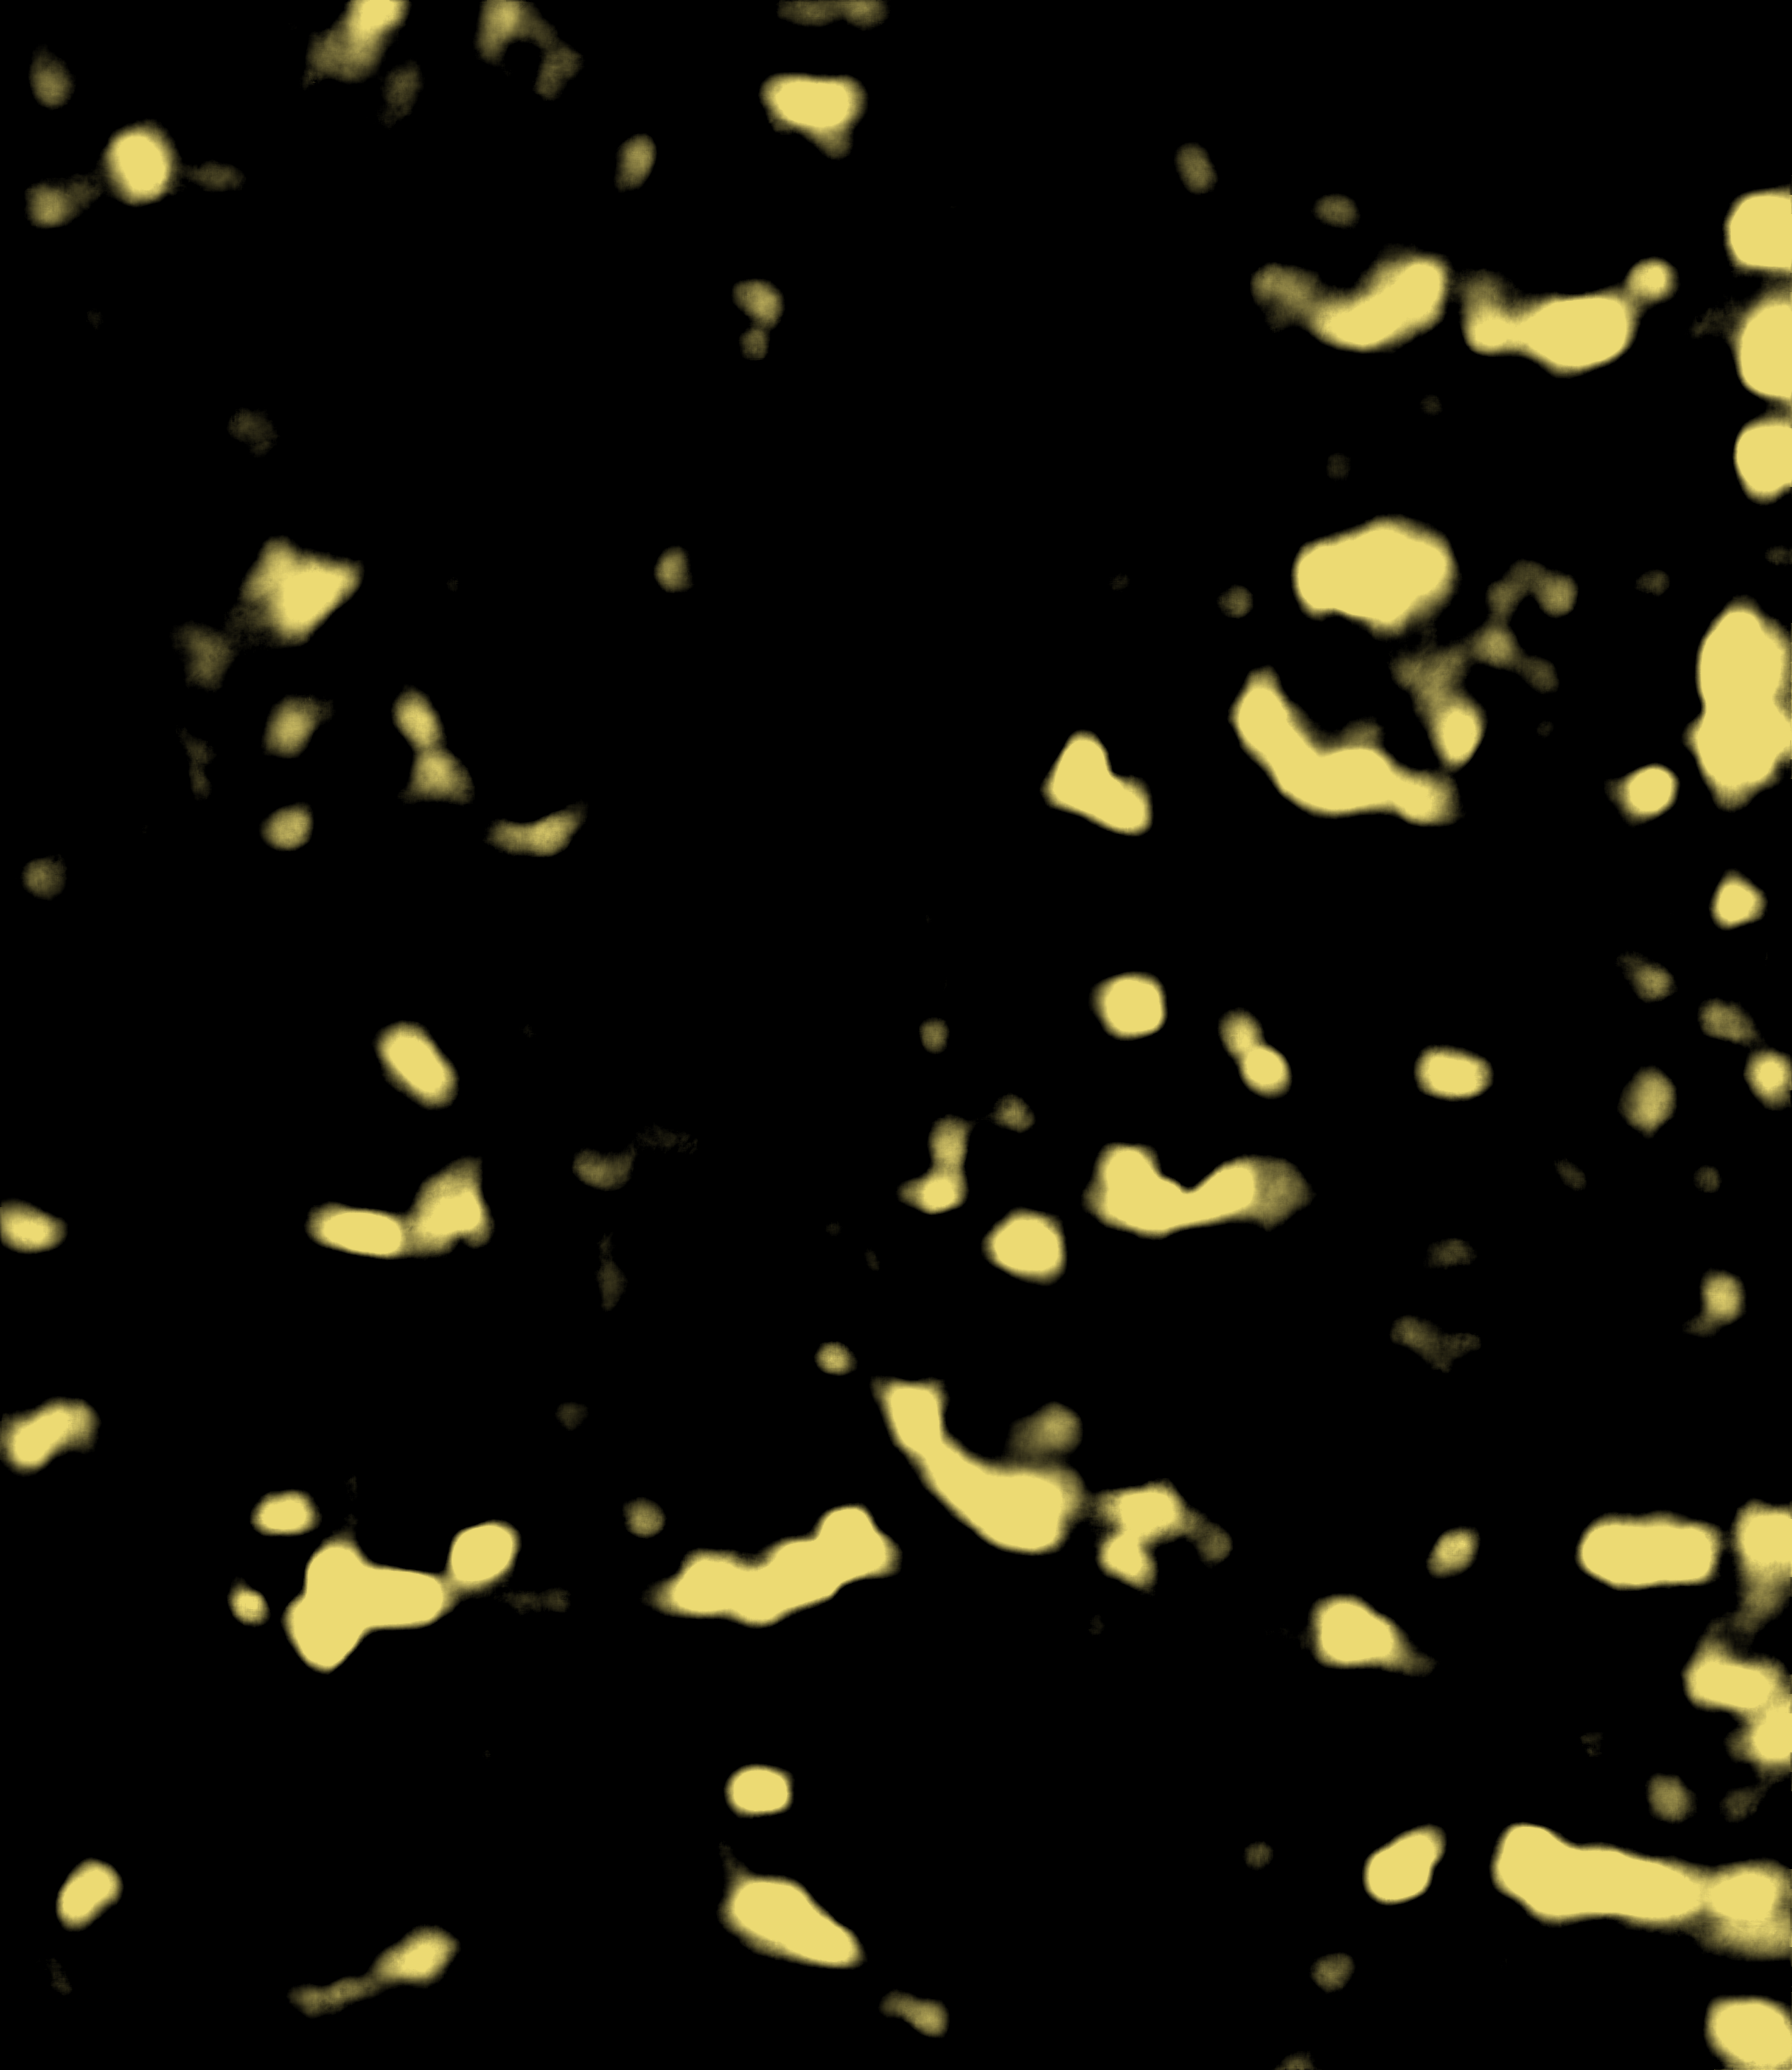
\includegraphics[width=122.48pt]{../figures/w060/w060_5_rectina-m1.png}}\end{minipage}}
\par\vspace{4pt}
\noindent\makebox[\columnwidth][c]{\begin{minipage}[t]{122.48pt}\centering\href{https://raw.githubusercontent.com/evilaliv3/vesuvius-challenge-pipeline/main/results/db27c806-rectina/src/figures/w060/w060_4_reader-v3.png}{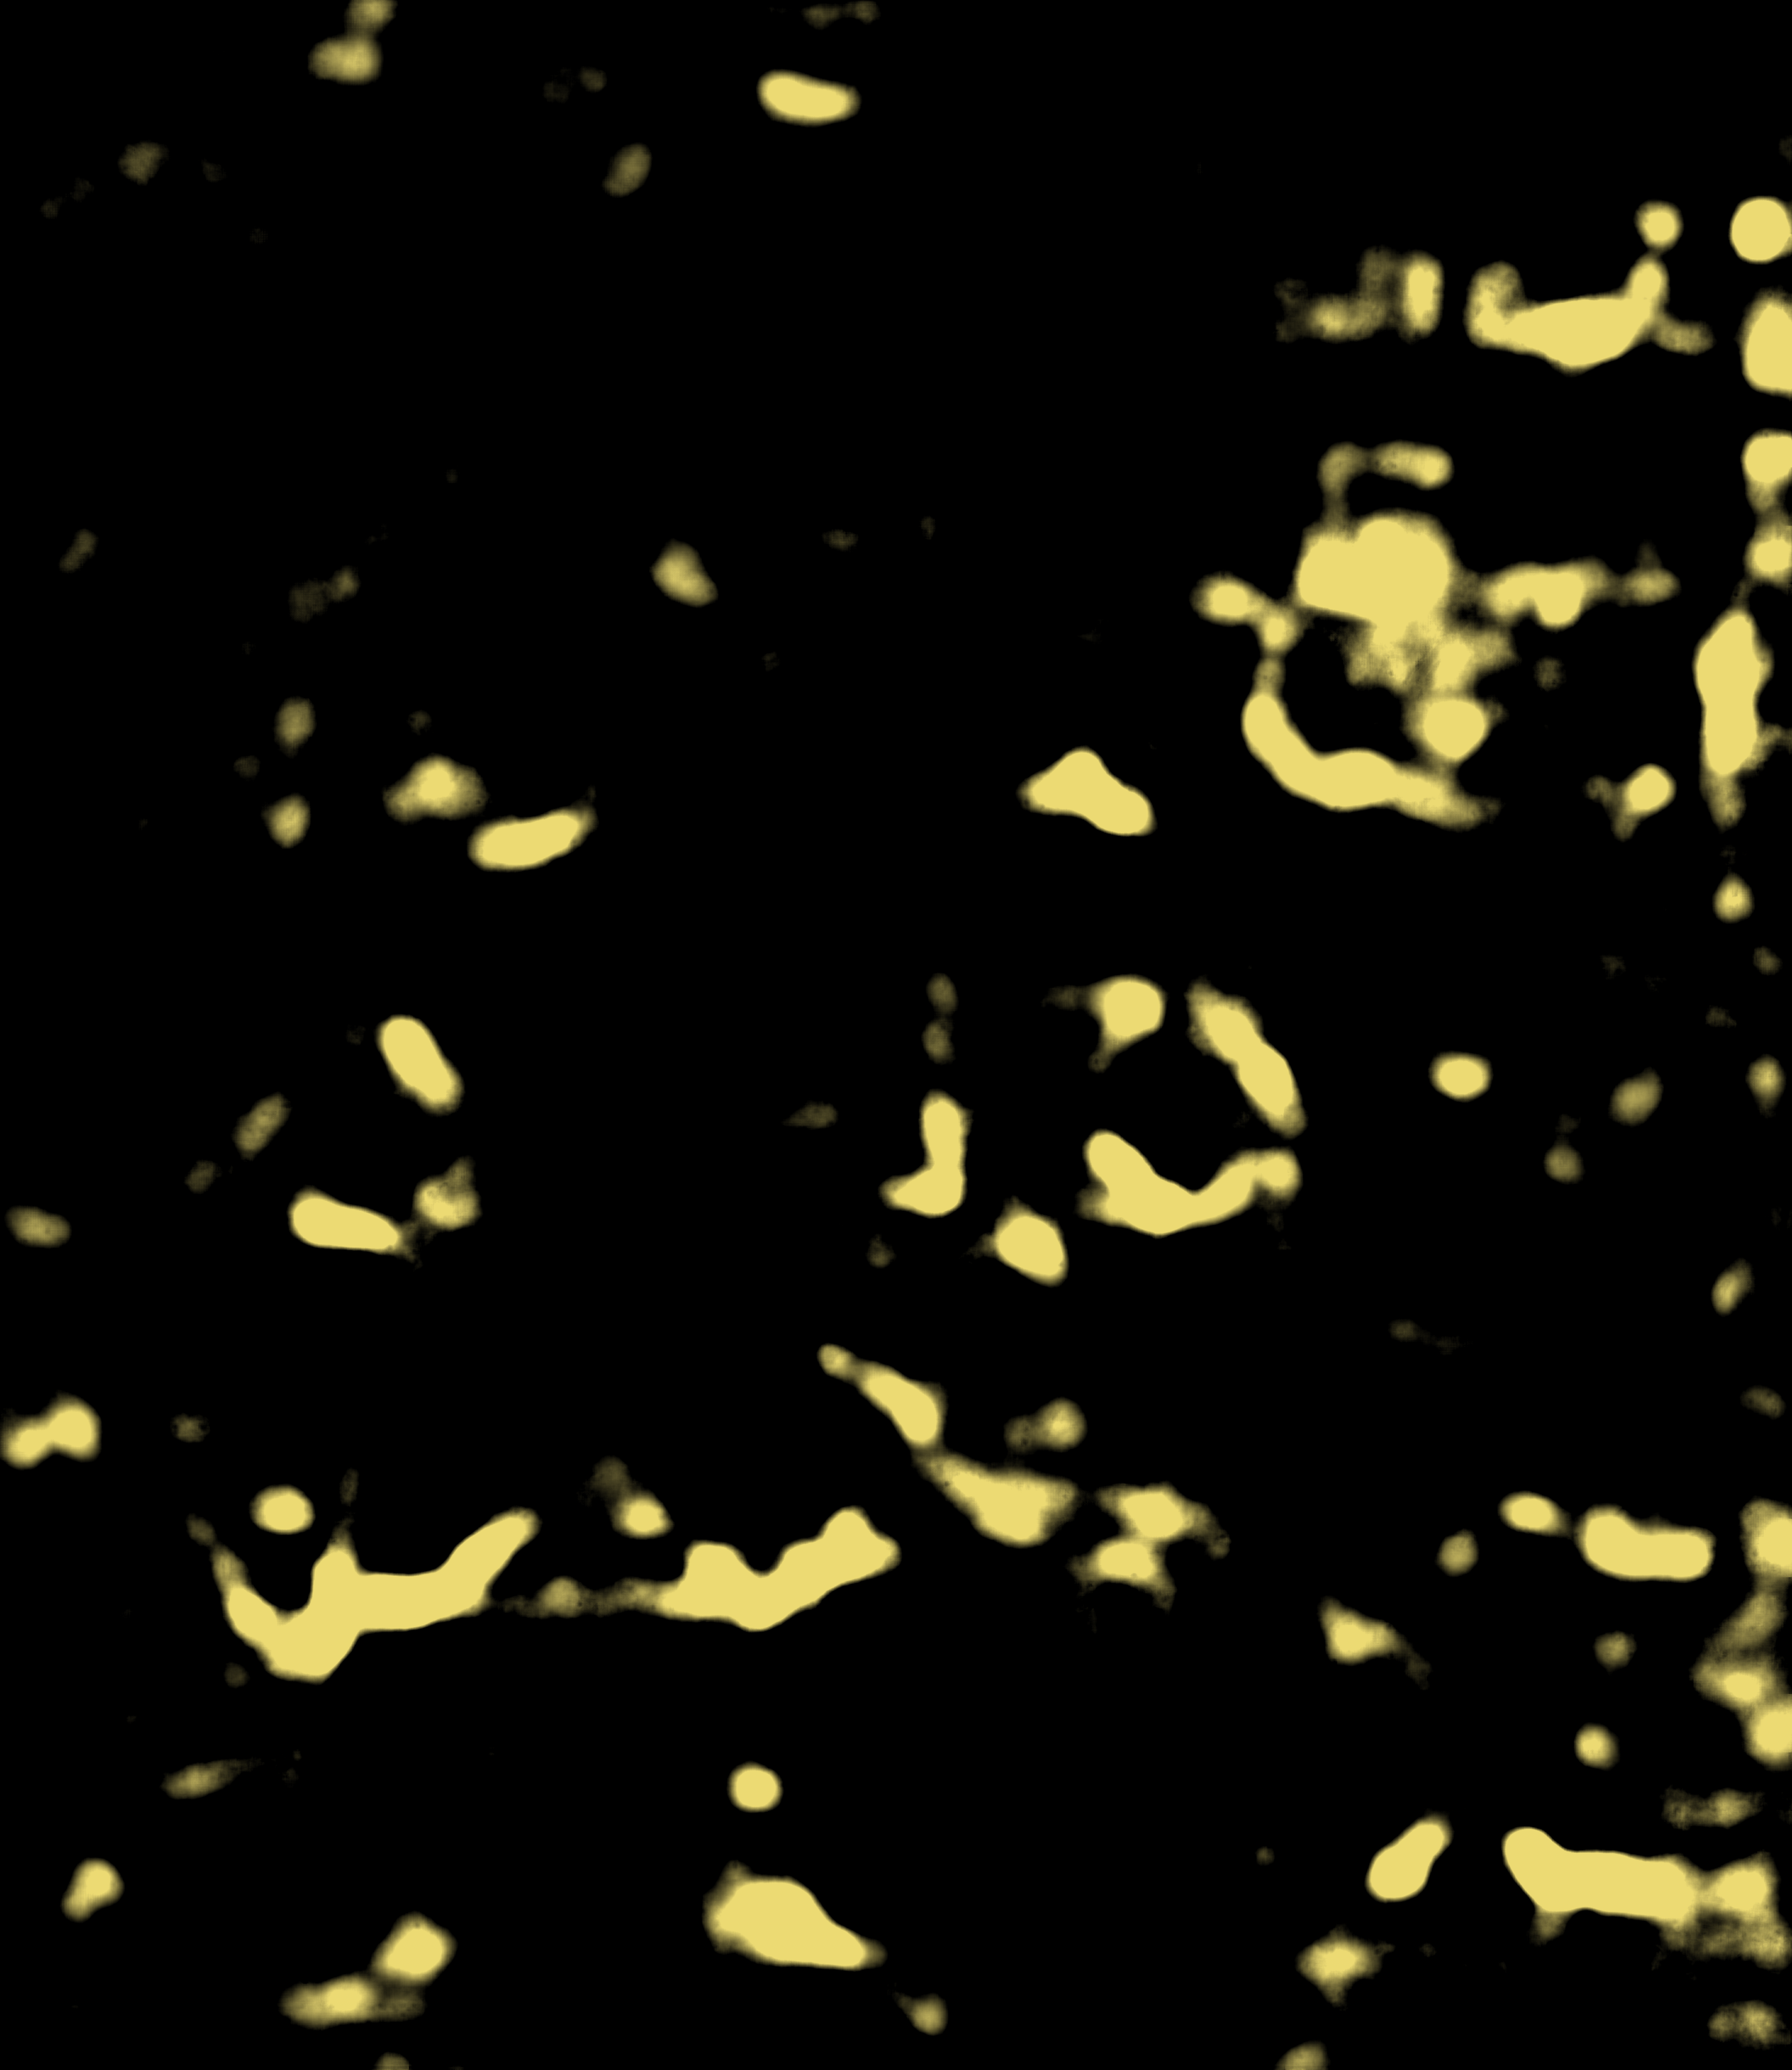
\includegraphics[width=122.48pt]{../figures/w060/w060_4_reader-v3.png}}\end{minipage}\hspace{2pt}\begin{minipage}[t]{122.48pt}\centering\href{https://raw.githubusercontent.com/evilaliv3/vesuvius-challenge-pipeline/main/results/db27c806-rectina/src/figures/w060/w060_6_rectina-m2.png}{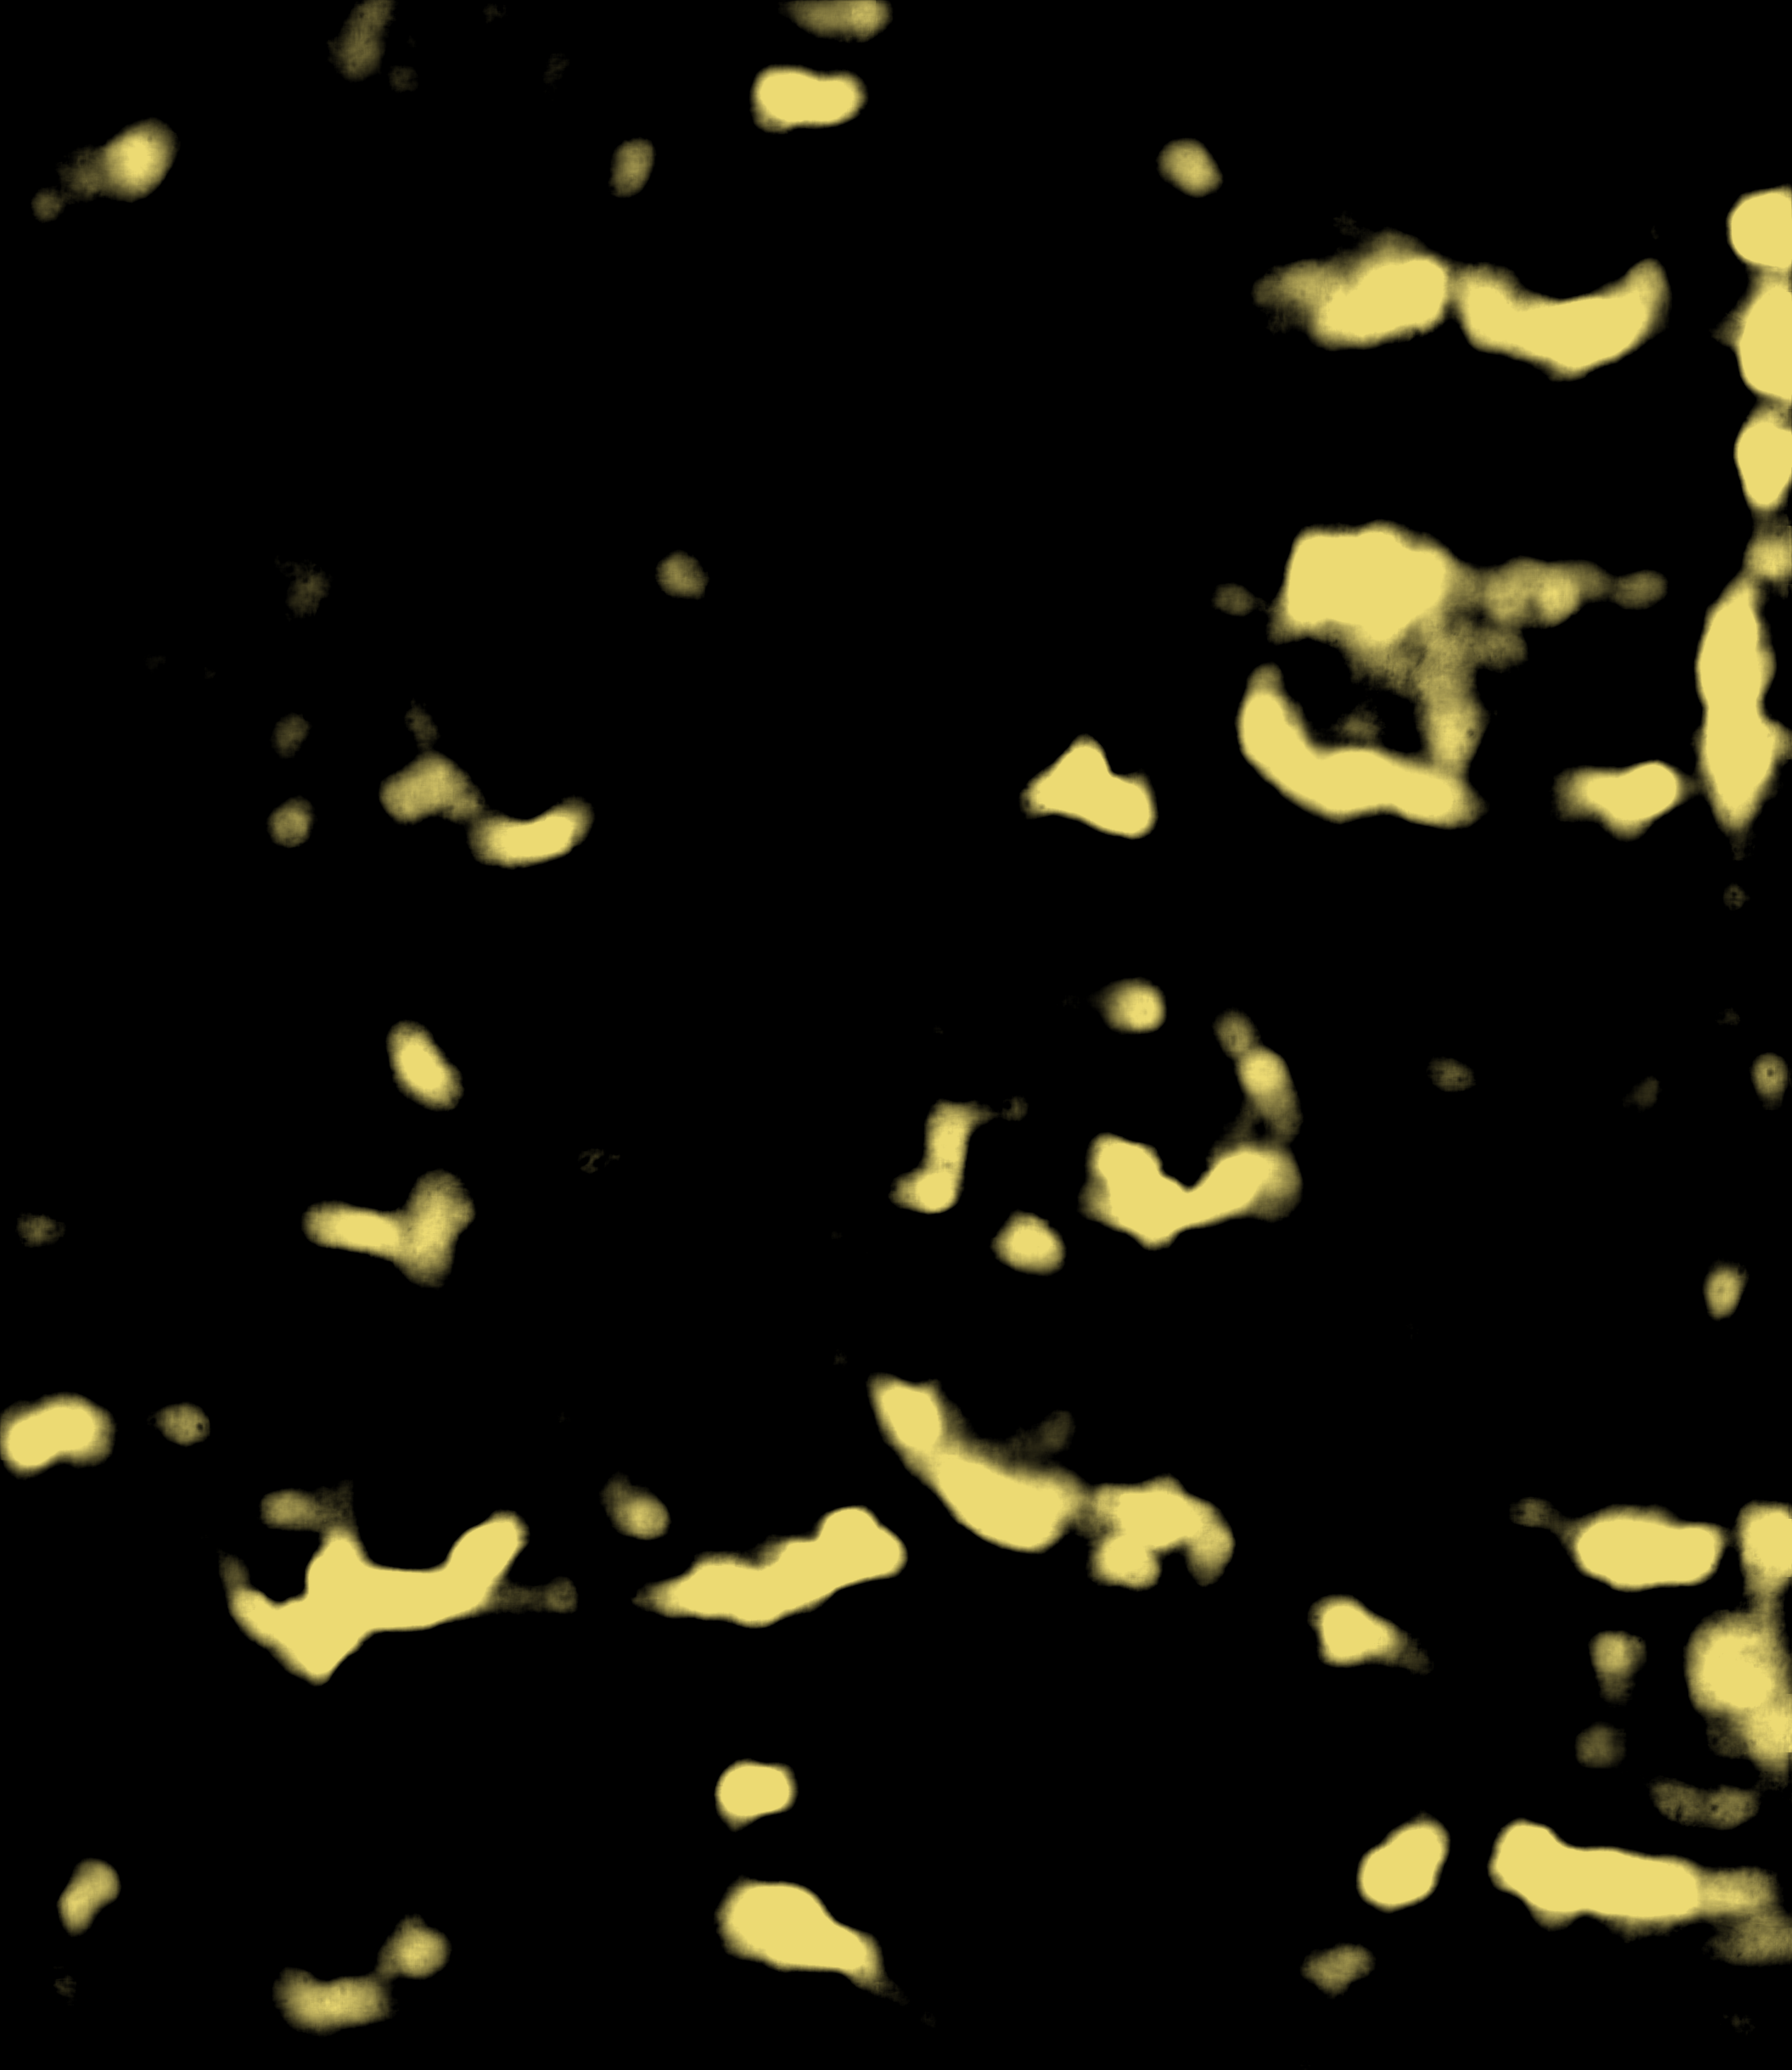
\includegraphics[width=122.48pt]{../figures/w060/w060_6_rectina-m2.png}}\end{minipage}}
\caption{Control unit 1447 w060, three rows of two panels. Row 1: left, Texture; right, Labels. Row 2: left, Reader v2; right, Rectina m1 (display windows: Reader v2 0.358837 to 0.460831 (ramp); Rectina m1 0.419819 to 0.580751 (ramp)). Row 3: left, Reader v3; right, Rectina m2 (display windows: Reader v3 0.381681 to 0.538574 (ramp); Rectina m2 0.465540 to 0.657352 (ramp)). Each map is stretched between its own percentiles. Reader and model stand side by side in the rows 2 and 3.}
\end{figure}

